%%%%%%%%%%%%%%%%%%%%%%%%%%%%%%%%%%%%%%%%%%%%%%%%%%%%%%%%%%%%%%%%%%%%%%%%%%%%%%%%%%%%%%%%%%%%%%%%%%%%%%%%%%%%%%%%%%%%%%%%%%%%%%%%%%%%%%%%%%%%%%%%%%%%%%%%%%%
% This is just an example/guide for you to refer to when submitting manuscripts to Frontiers, it is not mandatory to use Frontiers .cls files nor frontiers.tex  %
% This will only generate the Manuscript, the final article will be typeset by Frontiers after acceptance.   
%                                              %
%                                                                                                                                                         %
% When submitting your files, remember to upload this *tex file, the pdf generated with it, the *bib file (if bibliography is not within the *tex) and all the figures.
%%%%%%%%%%%%%%%%%%%%%%%%%%%%%%%%%%%%%%%%%%%%%%%%%%%%%%%%%%%%%%%%%%%%%%%%%%%%%%%%%%%%%%%%%%%%%%%%%%%%%%%%%%%%%%%%%%%%%%%%%%%%%%%%%%%%%%%%%%%%%%%%%%%%%%%%%%%

%%% Version 3.4 Generated 2022/06/14 %%%
%%% You will need to have the following packages installed: datetime, fmtcount, etoolbox, fcprefix, which are normally inlcuded in WinEdt. %%%
%%% In http://www.ctan.org/ you can find the packages and how to install them, if necessary. %%%
%%%  NB logo1.jpg is required in the path in order to correctly compile front page header %%%

\documentclass[utf8]{FrontiersinHarvard} % for articles in journals using the Harvard Referencing Style (Author-Date), for Frontiers Reference Styles by Journal: https://zendesk.frontiersin.org/hc/en-us/articles/360017860337-Frontiers-Reference-Styles-by-Journal
%\documentclass[utf8]{FrontiersinVancouver} % for articles in journals using the Vancouver Reference Style (Numbered), for Frontiers Reference Styles by Journal: https://zendesk.frontiersin.org/hc/en-us/articles/360017860337-Frontiers-Reference-Styles-by-Journal
%\documentclass[utf8]{frontiersinFPHY_FAMS} % Vancouver Reference Style (Numbered) for articles in the journals "Frontiers in Physics" and "Frontiers in Applied Mathematics and Statistics" 

%\setcitestyle{square} % for articles in the journals "Frontiers in Physics" and "Frontiers in Applied Mathematics and Statistics" 
\usepackage{url,hyperref,lineno,microtype,subcaption}
\usepackage[onehalfspacing]{setspace}
\usepackage{url,hyperref,lineno,microtype}
\usepackage[onehalfspacing]{setspace}
\linenumbers

\usepackage{nicefrac}
\usepackage[linesnumbered,lined,ruled,commentsnumbered]{algorithm2e}
\SetKwInOut{Input}{Initialization}

% used to format tables
\usepackage{makecell}


% Leave a blank line between paragraphs instead of using \\


\def\keyFont{\fontsize{8}{11}\helveticabold }
\def\firstAuthorLast{Oliveira Jr. {et~al.}} %use et al only if is more than 1 author
\def\Authors{Vanderlei C. Oliveira Jr.\,$^{1}$, Diego Takahashi\,$^{1}$, Andr{\'e} L. A. Reis\,$^{2}$ and Val{\'e}ria C. F. Barbosa\,$^{1,*}$}
% Affiliations should be keyed to the author's name with superscript numbers and be listed as follows: Laboratory, Institute, Department, Organization, City, State abbreviation (USA, Canada, Australia), and Country (without detailed address information such as city zip codes or street names).
% If one of the authors has a change of address, list the new address below the correspondence details using a superscript symbol and use the same symbol to indicate the author in the author list.
\def\Address{$^{1}$Observat{\'o}rio Nacional, Department of Geophysics, Rio de Janeiro, Brasil\\
$^{2}$Universidade do Estado do Rio de Janeiro, Department of Applied Geology, Rio de Janeiro, Brasil}
% The Corresponding Author should be marked with an asterisk
% Provide the exact contact address (this time including street name and city zip code) and email of the corresponding author
\def\corrAuthor{Val{\'e}ria C.F. Barbosa}

\def\corrEmail{valcris@on.br}

\begin{document}
\onecolumn
\firstpage{1}

\title {Computational aspects of the equivalent-layer technique: review} 

\author[\firstAuthorLast ]{\Authors} %This field will be automatically populated
\address{} %This field will be automatically populated
\correspondance{} %This field will be automatically populated

\extraAuth{}% If there are more than 1 corresponding author, comment this line and uncomment the next one.
%\extraAuth{corresponding Author2 \\ Laboratory X2, Institute X2, Department X2, Organization X2, Street X2, City X2 , State XX2 (only USA, Canada and Australia), Zip Code2, X2 Country X2, email2@uni2.edu}


\maketitle

%%% Manuscript body 
\begin{abstract}

\section{}
Equivalent-layer technique is a powerful tool for processing potential-field data in the space domain. However, the greatest hindrance for using the equivalent-layer technique is its high computational cost for processing massive data sets. The  large amount of computer memory usage to store the full  sensitivity matrix combined with the computational time required for matrix-vector multiplications and to solve the resulting linear system, are the main  drawbacks that made unfeasible the use of the equivalent-layer technique for a long time. More recently, the advances in computational power propelled the development of methods to overcome the heavy computational cost  associated with the equivalent-layer technique. We present  a comprehensive review of the computation aspects concerning the equivalent-layer technique addressing how previous works have been dealt with the computational cost of this technique. 
Historically, the high computational cost  of the equivalent-layer technique has been overcome by using a variety of strategies such as: moving data-window scheme,   column- and row-action updates of the 
sensitivity matrix, reparametrization, sparsity induction of the sensitivity matrix,  iterative methods using the full sensitivity matrix,  iterative deconvolution  by using the concept of  block-Toeplitz Toeplitz-block (BTTB) matrices and
direct deconvolution.
We compute the number of floating-point operations of some of these strategies adopted in the 
equivalent-layer technique to show their  effectiveness in reducing the computational demand. 
Numerically, we also address the stability of some of these strategies used in the equivalent-layer technique by comparing with the stability via the classic equivalent-layer technique with the zeroth-order Tikhonov regularization.
We show that even for the most computationally efficient methods, which can save up to $10^{9}$ flops, the stability of the linear system is maintained. 
The two most efficient strategies, iterative and direct deconvolutions, can process large datasets quickly and yield good results. 
However, direct deconvolution has some drawbacks. 
Real data from Carajás Mineral Province, Brazil, is also used to validate the results showing a potential field transformation.


\tiny
 \keyFont{ \section{Keywords:} equivalent layer, gravimetry, fast algorithms, computational cost, stability analysis} %All article types: you may provide up to 8 keywords; at least 5 are mandatory.
\end{abstract}

3333\section{Introduction}

The equivalent-layer technique has been used by exploration geophysicists for processing potential-field 
data since the late 1960s \citep{dampney1969}. 
This technique is based on a widely accepted principle, which states that a discrete set of observed 
potential-field data due to 3D sources 
can be approximated by that due to a discrete discrete set of virtual sources (such as point 
masses, dipoles, prisms, doublets). From a theoretical point of view, the equivalent-layer 
technique is grounded on potential theory \citep{kellogg1967} and consists in considering 
that the potential field data can be approximated by a linear combination of harmonic 
functions describing the potential field due to the virtual sources. These sources, commonly 
called equivalent sources, are arranged on a layer with finite horizontal dimensions and 
located below the observations. In the classical approach, a linear inverse problem is 
solved to estimate the physical property of each equivalent source subject to fit the 
observations. Then, the estimated physical-property distribution on the equivalent layer is 
used to accomplish the desired potential-field transformation (e.g., interpolation, 
upward/downward continuation, reduction to the pole). The later step is done by multiplying 
the estimated physical-property distribution by the matrix of Green's functions associated 
with the desired potential-field transformation.

Because the linear inverse problem to be solved in the equivalent-layer technique is set up 
with a full sensitivity matrix, its computational cost strongly depends on the number of 
potential-field observations and can be very inefficient for dealing with massive data sets. 
To overcome this problem, computationally efficient methods based on equivalent-layer 
technique have arose in the late 1980s. 
This comprehensive review discusses specific strategies aimed at reducing the computational cost of the equivalent-layer technique.
These strategies are addressed in the following articles: 
\cite{leao-silva1989};
\cite{cordell1992};
\cite{xia-etal1993};
\cite{mendonca-silva1994};  
\cite{guspi-novara2009};
\cite{li-oldenburg2010};
\cite{oliveirajr-etal2013};
\cite{siqueira-etal2017};
\cite{jirigalatu-ebbing2019};
\citet{takahashi-etal2020,takahashi-etal2022}
\cite{mendonca2020}; and
\cite{soler-uieda2021};


To our knowledge, the first method towards improving the efficiency  was proposed by \cite{leao-silva1989}, 
who used an overlapping moving-window scheme spanning the data set. 
The strategy adopted in \cite{leao-silva1989} involves solving several smaller, regularized linear 
inverse problems instead of one large problem. 
This strategy uses a small data window and distributes equivalent sources 
on a small regular grid at a constant depth below the data surface, with the sources' window extending beyond 
the boundaries of the data window.
Because of the spatial layouts of observed data and equivalent sources in \cite{leao-silva1989}, the small 
sensitivity submatrix containing the coordinates of the data and equivalent sources within a window remains 
constant for all data windows. This holds true regardless  of the specific locations of the data and equivalent 
sources within each window.
For each position of the data window, this scheme consists in computing the processed field 
at the center of the data window only, and the next estimates of the processed field are 
obtained by shifting the data window across the entire dataset. 
More recently, \cite{soler-uieda2021} extended the method introduced by \cite{leao-silva1989} to accommodate 
irregularly spaced data collected on a non-flat surface.
Unlike  \cite{leao-silva1989}, in the generalization proposed by \cite{soler-uieda2021}, the sensitivity 
submatrix that includes the coordinates of the data and equivalent sources needs to be computed for each window.
\cite{soler-uieda2021}  developed a computational approach to further enhance the efficiency of the 
equivalent-layer technique by combining two strategies. 
The first one --- the block-averaging source locations --- reduces the number of model parameters and the second 
strategy --- the gradient-boosted algorithm --- reduces the size of the linear system to be solved by 
iteratively fitting the equivalent source model along overlapping windows. 
It is worth noting that the equivalent-layer strategy of using a moving-window scheme either in 
\cite{leao-silva1989} or in \cite{soler-uieda2021} is similar to discrete convolution.

As another strategy to reduce the computational workload of the equivalent-layer technique, some authors 
have employed column- and row-action updates, which are commonly applied to image reconstruction methods \citep[e.g.,][]{elfving-etal2017}. 
These methods involve iterative calculations of a single column and a single row of the sensitivity matrix, respectively.
Following the strategy column-action update, \cite{cordell1992} proposed a computational method in which a single equivalent source positioned below a measurement station is iteratively used to compute both the predicted data and residual data for all stations. 
In  \citeauthor{cordell1992}'s method, a single column of the sensitivity matrix is calculated per iteration, meaning that a single equivalent source contributes to data fitting in each iteration. 
\cite{guspi-novara2009} further extended  \citeauthor{cordell1992}'s method 
by applying it to scattered magnetic observations.
Following the strategy of column-action update, \cite{mendonca-silva1994} developed an iterative procedure where one data point is incorporated at a time, and a single row of the sensitivity matrix is calculated per iteration.
This strategy adopted by \cite{mendonca-silva1994} is known as \textit{equivalent data concept}.
This concept is based on the principle that certain data points within a dataset are redundant and, as a result, do not contribute to the final solution
On the other hand, there is a subset of observations known as equivalent data, which effectively contributes to the final solution and fits the remaining redundant data. 
In their work, \cite{mendonca-silva1994} adopted an iterative approach to select a substantially smaller subset of equivalent data from the original dataset. 


The next strategy involves reparametrizing the equivalent layer with the objective of solving a 
smaller linear inverse problem by reducing the dimension of the model space.
\cite{oliveirajr-etal2013} reduced the model parameters by approximating the equivalent-source layer by a piecewise-polynomial function defined on a set of user-defined small equivalent-source windows. 
The estimated parameters are the polynomial coefficients for each window and they are much smaller than the original number of equivalent sources.
By using the subspace method, \cite{mendonca2020} reparametrizes the equivalent layer, which involves 
reducing the dimension of the linear system from the original parameter-model space to a lower-dimensional subspace.
The subspace bases span the parameter-model space and they are constructed by applying the singular value decomposition to the matrix containing the gridded data.

Following the strategy of sparsity induction, 
\cite{li-oldenburg2010} transformed the full sensitivity matrix into a sparse one using orthonormal compactly supported wavelets. 
\cite{barnes-lumley2011} proposed an alternative approach to introduce sparsity based on the use of 
quadtree discretization to group equivalent sources far from the computation points.
Those authors explore the induced sparsity by using specific iterative methods to solve the linear system.

The strategy named iterative methods estimates iteratively the parameter vector that represents a distribution over an equivalent layer.
\cite{xia-sprowl1991} and \cite{xia-etal1993} have developed efficient iterative algorithms 
for updating the distribution of physical properties within the equivalent layer in the wavenumber and space domains, respectively.
Specifically, in \citeauthor{xia-sprowl1991}'s (\citeyear{xia-sprowl1991}) method the physical-property distribution is updated by using the ratio between the squared depth to the equivalent source and the gravitational constant multiplied by the residual between the observed and predicted observation at the measurement station. 
\cite{siqueira-etal2017} developed an iterative solution where the sensitivity matrix is transformed into a diagonal matrix with constant terms through the use of the \textit{excess mass criterion} and of the positive correlation between the observed gravity data and the masses on the equivalent layer.
The fundamentals of the \citeauthor{siqueira-etal2017}'s method
is  based on the Gauss' theorem \cite[e.g.,][p. 43]{kellogg1967} and the total excess of mass \cite[e.g.,][p. 60]{blakely1996}.
All these iterative methods use the full and dense sensitivity matrix to calculate the predicted data 
and residual data in the whole survey data per iteration.
Hence, the iterative methods proposed by \cite{xia-sprowl1991}, \cite{xia-etal1993} and 
\cite{siqueira-etal2017} neither compress nor reparametrize the sensitivity  matrix.
\cite{jirigalatu-ebbing2019} also proposed an iterative equivalent layer that uses the full and dense sensitivity matrix. 
However, in their approach, \cite{jirigalatu-ebbing2019}  efficiently compute  the predicted data and 
residual data for the entire survey per iteration in the wavenumber domain.

Following the strategy of the  iterative deconvolution, \citet{takahashi-etal2020,takahashi-etal2022}
developed fast and effective equivalent-layer techniques for processing, respectively, gravity and magnetic data by modifying the forward modeling to 
estimate the physical-property distribution over the equivalent layer through a 2D discrete fast convolution.
These methods took advantage of the Block-Toeplitz Toeplitz-block (BTTB) structure of the sensitivity matrices, allowing them to be calculated by 
using only their first column.
In practice, the forward modeling uses a single equivalent source, which significantly reduces the required RAM memory. 

The method introduced by \citet{takahashi-etal2020,takahashi-etal2022} can be reformulated to eliminate the need for conjugate gradient iterations. 
This reformulation involves employing a \textit{direct deconvolution} approach \citep[e.g.,][p. 220]{aster_etal2019} with 
\textit{Wiener filter} \citep[e.g.,][p. 263]{gonzalez-woods2002}.

Here, we present a comprehensive review of diverse strategies to solve the linear system of the equivalent layer alongside an analysis 
of the computational cost and stability of these strategies. 
To do this analysis, we are using the floating-point operations count to evaluate the performance of 
a selected set of methods (e.g., \cite{\cite{leao-silva1989};  \cite{cordell1992};
\cite{oliveirajr-etal2013}; \cite{siqueira-etal2017}; \cite{mendonca2020}; \cite{takahashi-etal2020}; 
\cite{soler-uieda2021}; and direct deconvolution). 
To test the stability, we are using the linear system sensitivity to noise as a comparison parameter for the fastest of these methods alongside the classical normal equations. 
A potential-field transformation will also be used to evaluate the quality of the equivalent sources estimation results using both synthetic and real data from Carajás Mineral Province, Brazil.

In the following sections, we will address the theoretical bases of the equivalent-layer technique, including aspects such as the sensitivity matrix, layer depth and spatial distribution and the total number of equivalent sources. 
Then, we will explore the general formulation and solution of the linear inverse problem for the equivalent-layer technique, including discussions on linear system solvers. 
Additionally, we will quantify the required arithmetic operations for a given equivalent-layer method, assessing the number of floating-point operations involved. 
Next, we will evaluate the stability of the estimated solutions obtained from applying specific equivalent-layer methods.
Finally, we will delve into the computational strategies adopted in the equivalent-layer technique for reducing computational costs. 
These strategies encompass various approaches, such as the moving data-window scheme, column- and row-action updates of the sensitivity matrix, reparametrization, sparsity induction of the sensitivity matrix, iterative methods using the full sensitivity matrix, iterative deconvolution using the concept of block-Toeplitz Toeplitz-block (BTTB) matrices, and direct deconvolution.


\section{Fundamentals}

Let $\mathbf{d}$ be a $D \times 1$ vector, whose $i$-th element $d_{i}$ is the observed potential
field at the position $(x_{i}, y_{i}, z_{i})$, $i \in \{1:D\}$, of a topocentric Cartesian system with
$x$, $y$ and $z$ axes pointing to north, east and down, respectively.
Consider that $d_{i}$ can be satisfactorily approximated by a harmonic function
\begin{equation}
	f_{i} = \sum\limits_{j = 1}^{P} g_{ij} \, p_{j} \: ,
	\quad i \in \{1:D\} \: ,
	\label{eq:predicted-data-f-i}
\end{equation}
where, $p_{j}$ represents the scalar physical property of a virtual source (i.e., monopole, dipole, prism) located
at $(x_{j}, y_{j}, z_{j})$, $j \in \{1:P\}$ and 
\begin{equation}
	g_{ij} \equiv g(x_{i} - x_{j}, y_{i} - y_{j}, z_{i} - z_{j}) \: ,
	\quad z_{i} < \min\{z_{j}\} \: , \quad \forall i \in \{1:D\} \: ,
	\label{eq:harmonic-function-g-ij}
\end{equation}
is a harmonic function, where $\min\{z_{j}\}$ denotes the minimum $z_{j}$, or the vertical coordinate of the 
shallowest virtual source.
These virtual sources are called \textit{equivalent sources} and they form an \textit{equivalent layer}.
In matrix notation, the potential field produced by all equivalent sources at all points 
$(x_{i}, y_{i}, z_{i})$, $i \in \{1:D\}$, is given by:
\begin{equation}
	\mathbf{f} = \mathbf{G} \mathbf{p} \: ,
	\label{eq:predicted-data-vector}
\end{equation}
where $\mathbf{p}$ is a $P \times 1$ vector with $j$-th element $p_{j}$ representing the scalar physical property
of the $j$-th equivalent source 
and $\mathbf{G}$ is a $D \times P$ matrix with element $g_{ij}$ given by equation \ref{eq:harmonic-function-g-ij}. 

The equivalent-layer technique consists in solving a linear inverse problem to determine a parameter vector $\mathbf{p}$ 
leading to a predicted data vector $\mathbf{f}$ (equation \ref{eq:predicted-data-vector}) \textit{sufficiently close to} the 
observed data vector $\mathbf{d}$, whose $i$-th element $d_{i}$ is the observed potential field at $(x_{i}, y_{i}, z_{i})$.
The notion of \textit{closeness} is intrinsically related to the concept of \textit{vector norm} \cite[e.g.,][p. 68]{golub-vanloan2013}
or \textit{measure of length} \cite[e.g.,][p. 41]{menke2018}.
Because of that, almost all methods for determining $\mathbf{p}$ actually estimate a parameter 
vector $\tilde{\mathbf{p}}$ minimizing a length measure of the difference between $\mathbf{f}$ and $\mathbf{d}$
(see subsection \ref{subsec:general-formulation}).
Given an estimate $\tilde{\mathbf{p}}$, it is then possible to compute a potential field transformation 
\begin{equation}
	\mathbf{t} = \mathbf{A} \tilde{\mathbf{p}} \: ,
	\label{eq:transformation}
\end{equation}
where $\mathbf{t}$ is a $T \times 1$ vector with $k$-th element $t_{k}$ representing the transformed potential field at
the position $(x_{k}, y_{y}, z_{k})$, $k \in \{1:T\}$, and
\begin{equation}
	a_{kj} \equiv a(x_{k} - x_{j}, y_{k} - y_{j}, z_{k} - z_{j}) \: ,
	\quad z_{k} < \min\{z_{j}\} \: , \quad \forall k \in \{1:T\} \: ,
	\label{eq:harmonic-function-a-kj}
\end{equation}
is a harmonic function representing the $kj$-th element of the $T \times P$ matrix $\mathbf{A}$.

\subsection{Spatial distribution and total number of equivalent sources}
\label{subsec:spatial-distribution-sources}

There is no well-established criteria to define the optimum number $P$ or the spatial distribution
of the equivalent sources. We know that setting an equivalent layer with more (less) sources than potential-field 
data usually leads to an underdetermined (overdetermined) inverse problem \cite[e.g.,][ p. 52--53]{menke2018}.
Concerning the spatial distribution of the equivalent sources, the only condition is that they must rely on a 
surface that is located below and does not cross that containing the potential field data.
\citet{soler-uieda2021} present a practical discussion about this topic.

From a theoretical point of view, the equivalent layer reproducing a given potential field data set cannot cross the
true gravity or magnetic sources. This condition is a consequence of recognizing that the equivalent layer is essentially an indirect solution of 
a boundary value problem of potential theory \citep[e.g.,][]{roy1962,zidarov1965,dampney1969,li_etal_2014,reis-etal2020}.
In practical applications, however, there is no guarantee that this condition is satisfied. 
Actually, its is widely known from practical experience \cite[e.g.,][]{gonzalez-etal2022} that the equivalent-layer technique
works even for the case in which the layer cross the true sources. 

Regarding the depth of the equivalent layer, \citet{dampney1969}  proposed a criterion based on horizontal data sampling, 
suggesting that the equivalent-layer depth should be between two and six times the horizontal grid spacing, 
considering evenly spaced data. 
However, when dealing with a survey pattern that has unevenly spaced data, \citet{reis-etal2020} adopted an alternative 
empirical criterion. 
According to their proposal, the depth of the equivalent layer should range from two to three times the spacing between 
adjacent flight lines.
The criteria of \citet{dampney1969} and \citet{reis-etal2020} are valid for planar equivalent layers. 
\citet{cordell1992} have proposed and an alternative criterion for scattered data that leads to an undulating equivalent layer.
This criterion have been slightly modified by \citet{guspi-etal2004}, \citet{guspi-novara2009} and \citet{soler-uieda2021},
for example, and consists in setting one equivalent source below each datum at a depth 
proportional to the horizontal distance to the nearest neighboring data points.
\citet{soler-uieda2021} have compared different strategies for defining the equivalent sources depth for the specific
problem of interpolating gravity data, but they have not found significant differences between them.
Regarding the horizontal layout, \cite{soler-uieda2021} proposed the block-averaged sources locations 
in which the survey area is divided into horizontal blocks and one single equivalent source is assigned to each block. 
The horizontal coordinates of the single source in a given block is defined by the average horizontal 
coordinates of the observation points at the block. 
According to \cite{soler-uieda2021}, this block-averaged layout may prevent aliasing of the interpolated 
values, specially when the observations are unevenly sampled.
This strategy also reduces the number of equivalent sources without affecting the accuracy of the potential-field interpolation. 
Besides, it reduces the computational load for estimating the physical property on the equivalent layer.

\subsection{Matrix $\mathbf{G}$}
\label{subsec:sensitivity-matrix}

Generally, the harmonic function $g_{ij}$ (equation \ref{eq:harmonic-function-g-ij}) is defined in terms of the 
inverse distance between the observation point $(x_{i}, y_{i}, z_{i})$ and the $j$-th equivalent source at $(x_{j}, y_{j}, z_{j})$,
\begin{equation}
	\frac{1}{r_{ij}} \equiv \frac{1}{\sqrt{(x_{i} - x_{j})^{2} + (y_{i} - y_{j})^{2} + (z_{i} - z_{j})^{2}}} \: ,
	\label{eq:inverse-distance-ij}
\end{equation}
or by its partial derivatives of first and second orders, respectively given by
\begin{equation}
	\partial_{\alpha} \frac{1}{r_{ij}} \equiv \frac{-(\alpha_{i} - \alpha_{j})}{r_{ij}^{3}} \: ,
	\quad \alpha \in \{ x, y, z \} \: ,
	\label{eq:deriv-1-inverse-distance-ij}
\end{equation}
and
\begin{equation}
	\partial_{\alpha\beta} \frac{1}{r_{ij}} \equiv 
	\begin{cases}
		\frac{3 \, (\alpha_{i} - \alpha_{j})^{2}}{r_{ij}^{5}} \: , &\alpha = \beta \: , \\
		\frac{3 \, (\alpha_{i} - \alpha_{j}) \, (\beta_{i} - \beta_{j})}{r_{ij}^{5}} - \frac{1}{r_{ij}^{3}} \: , &\alpha \ne \beta \: , \\
	\end{cases}
	\quad \alpha, \beta \in \{ x, y, z \} \: .
	\label{eq:deriv-2-inverse-distance-ij}
\end{equation}
In this case, the equivalent layer is formed by punctual sources representing monopoles or dipoles
\cite[e.g.,][]{dampney1969, emilia1973, leao-silva1989, cordell1992, oliveirajr-etal2013, siqueira-etal2017, reis-etal2020, takahashi-etal2020, soler-uieda2021, takahashi-etal2022}.
Another common approach consists in not defining $g_{ij}$ by using equations \ref{eq:inverse-distance-ij}--\ref{eq:deriv-2-inverse-distance-ij},
but other harmonic functions obtained by integrating them over the volume of regular prisms 
\cite[e.g.,][]{li-oldenburg2010, barnes-lumley2011, li_etal_2014, jirigalatu-ebbing2019}.
There are also some less common approaches defining the harmonic function $g_{ij}$ (equation \ref{eq:harmonic-function-g-ij})
as the potential field due to plane faces with constant physical property \citep{hansen-miyazaki1984}, doublets \citep{silva1986} or
by computing the double integration of the inverse distance function with respect to $z$ \citep{guspi-novara2009}.

A common assumption for most of the equivalent-layer methods is that the harmonic function $g_{ij}$ 
(equation \ref{eq:harmonic-function-g-ij}) is independent on the actual physical relationship between the
observed potential field and their true sources \cite[e.g.,][]{cordell1992, guspi-novara2009,li_etal_2014}.
Hence, $g_{ij}$ can be defined according to the problem.
The only condition imposed to this function is that it decays to zero as the observation point $(x_{i}, y_{i}, z_{i})$
goes away from the position $(x_{j}, y_{j}, z_{j})$ of the $j$-th equivalent source.
However, several methods use a function $g_{ij}$ that preserves the physical relationship between the
observed potential field and their true sources.
For the case in which the observed potential field is gravity data, $g_{ij}$ is commonly defined as a component of 
the gravitational field produced at $(x_{i}, y_{i}, z_{i})$ by a point mass or prism located at $(x_{j}, y_{j}, z_{j})$, with unit density.
On the other hand, $g_{ij}$ is commonly defined as a component of the 
magnetic induction field produced at $(x_{i}, y_{i}, z_{i})$ by a dipole or prism located at $(x_{j}, y_{j}, z_{j})$,
with unit magnetization intensity, when the observed potential field is magnetic data.

The main challenge in the equivalent-layer technique is the computational complexity associated with handling large datasets. 
This complexity arises because the sensitivity matrix $\mathbf{G}$ (equation \ref{eq:predicted-data-vector}) is dense regardless of the 
harmonic function $g_{ij}$ (equation \ref{eq:harmonic-function-g-ij}) employed. 
In the case of scattered potential-field data, the structure of $\mathbf{G}$  is not well-defined, regardless of the spatial distribution 
of the equivalent sources.
However, in a specific scenario where (i) each potential-field datum is directly associated with a single equivalent source located directly below it, 
and (ii) both the data and sources are based on planar and regularly spaced grids,  \citet{takahashi-etal2020,takahashi-etal2022} demonstrate that 
$\mathbf{G}$ exhibits a block-Toeplitz Toeplitz-block (BTTB) structure. 
In such cases, the product of $\mathbf{G}$ and an arbitrary vector can be efficiently computed using a 2D fast Fourier transform as a discrete convolution.

\section{Linear inverse problem of equivalent-layer technique}
\label{sec:linear-inverse-problem}

\subsection{General formulation}
\label{subsec:general-formulation}

A general formulation for almost all equivalent-layer methods can be achieved by first considering 
that the $P \times 1$ parameter vector $\mathbf{p}$ (equation \ref{eq:predicted-data-vector}) can be reparameterized 
into a $Q \times 1$ vector $\mathbf{q}$ according to:
\begin{equation}
	\mathbf{p} = \mathbf{H} \, \mathbf{q} \: ,
	\label{eq:reparameterization}
\end{equation}
where $\mathbf{H}$ is a $P \times Q$ matrix.
The predicted data vector $\mathbf{f}$ (equation \ref{eq:predicted-data-vector}) can then be
rewritten as follows:
\begin{equation}
	\mathbf{f} = \mathbf{G} \, \mathbf{H} \, \mathbf{q} \: .
	\label{eq:predicted-data-vetor-reparameterized}
\end{equation}
Note that the original parameter vector $\mathbf{p}$ is defined in a $P$-dimensional space whereas the reparameterized
parameter vector $\mathbf{q}$ (equation \ref{eq:reparameterization}) lies in a $Q$-dimensional space.
For convenience, we use the terms $P$-space and $Q$-space to designate them.

In this case, the problem of estimating a parameter vector $\tilde{\mathbf{p}}$ minimizing a length 
measure of the difference between $\mathbf{f}$ (equation \ref{eq:predicted-data-vector}) and $\mathbf{d}$
is replaced by that of estimating an auxiliary vector $\tilde{\mathbf{q}}$ minimizing the goal function
\begin{equation}
	\Gamma(\mathbf{q}) = \Phi(\mathbf{q}) + \mu \: \Theta(\mathbf{q}) \: ,
	\label{eq:function-Gamma}
\end{equation}
which is a combination of particular measures of length given by
\begin{equation}
	\Phi(\mathbf{q}) = \left( \mathbf{d} - \mathbf{f} \right)^{\top}\mathbf{W}_{d}\left( \mathbf{d} - \mathbf{f} \right) \: ,
	\label{eq:function-Phi}
\end{equation}
and
\begin{equation}
	\Theta(\mathbf{q}) = \left( \mathbf{q} - \bar{\mathbf{q}} \right)^{\top}\mathbf{W}_{q}\left( \mathbf{q} - \bar{\mathbf{q}} \right) \: ,
	\label{eq:function-Theta}
\end{equation}
where the regularization parameter $\mu$ is a positive scalar controlling the trade-off between the data-misfit function 
$\Phi(\mathbf{q})$ and the regularization function $\Theta(\mathbf{q})$; 
$\mathbf{W}_{d}$ is a $D \times D$ symmetric matrix defining the relative importance of each observed datum $d_{i}$;
$\mathbf{W}_{q}$ is a $Q \times Q$ symmetric matrix imposing prior information on $\mathbf{q}$;
and $\bar{\mathbf{q}}$ is a $Q \times 1$ vector of reference values for $\mathbf{q}$ that satisfies
\begin{equation}
	\bar{\mathbf{p}} = \mathbf{H} \, \bar{\mathbf{q}} \: ,
	\label{eq:reparameterization-reference}
\end{equation}
where $\bar{\mathbf{p}}$ is a $P \times 1$ vector containing reference values
for the original parameter vector $\mathbf{p}$.

After obtaining an estimate $\tilde{\mathbf{q}}$ for the reparameterized parameter vector $\mathbf{q}$ (equation \ref{eq:reparameterization}), 
the estimate $\tilde{\mathbf{p}}$ for the original parameter vector 
(equation \ref{eq:predicted-data-vector}) is computed by 
\begin{equation}
	\tilde{\mathbf{p}} = \mathbf{H} \, \tilde{\mathbf{q}} \: .
	\label{eq:vector-p-tilde}
\end{equation}

The reparameterized vector $\tilde{\mathbf{q}}$ is obtained by first computing the gradient of $\Gamma(\mathbf{q})$,
\begin{equation}
	\boldsymbol{\nabla} \Gamma(\mathbf{q}) = 
	-2 \, \mathbf{H}^{\top}\mathbf{G}^{\top} \mathbf{W}_{d} \left(\mathbf{d} - \mathbf{f} \right) +
	2 \, \mu \, \mathbf{W}_{q} \left( \mathbf{q} - \bar{\mathbf{q}} \right) \: .
	\label{eq:gradient-Gamma}
\end{equation}
Then, by considering that $\boldsymbol{\nabla} \Gamma(\tilde{\mathbf{q}}) = \mathbf{0}$ (equation \ref{eq:gradient-Gamma}),
where $\mathbf{0}$ is a vector of zeros, as well as adding and subtracting the term
$\left( \mathbf{H}^{\top}\mathbf{G}^{\top}\mathbf{W}_{d} \mathbf{G} \, \mathbf{H} \right) \bar{\mathbf{q}}$ ,
we obtain
\begin{equation}
	\tilde{\boldsymbol{\delta}}_{q} = \mathbf{B} \, \boldsymbol{\delta}_{d} \: ,
	\label{eq:vector-q-tilde}
\end{equation}
where 
\begin{equation}
	\tilde{\mathbf{q}} = \tilde{\boldsymbol{\delta}}_{q} + \bar{\mathbf{q}} \: ,
	\label{eq:delta-q-tilde}
\end{equation}
\begin{equation}
	\boldsymbol{\delta}_{d} = \mathbf{d} - \mathbf{G} \, \mathbf{H} \, \bar{\mathbf{q}} \: ,
	\label{eq:delta-d}
\end{equation}
\begin{equation}
	\mathbf{B} = \left( \mathbf{H}^{\top} \mathbf{G}^{\top} \mathbf{W}_{d} \, \mathbf{G} \, \mathbf{H} + 
	\mu \, \mathbf{W}_{q} \right)^{-1}
	\mathbf{H}^{\top} \mathbf{G}^{\top} \mathbf{W}_{d} \: ,
	\label{eq:matrix-B-overdetermined}
\end{equation}
or, equivalently \cite[][p. 62]{menke2018},
\begin{equation}
	\mathbf{B} = \mathbf{W}_{q}^{-1} \, \mathbf{H}^{\top} \mathbf{G}^{\top}
	\left( \mathbf{G} \, \mathbf{H} \, \mathbf{W}_{q}^{-1} \,
	\mathbf{H}^{\top}\mathbf{G}^{\top} + \mu \mathbf{W}_{d}^{-1} \right)^{-1} \: .
	\label{eq:matrix-B-underdetermined}
\end{equation}
Evidently, we have considered that all inverses exist in equations \ref{eq:matrix-B-overdetermined} and \ref{eq:matrix-B-underdetermined}.

The $Q \times D$ matrix $\mathbf{B}$ defined by equation \ref{eq:matrix-B-overdetermined} is commonly used for the case 
in which $D > Q$, i.e., when there are more data than parameters (overdetermined problems).
In this case, we consider that the estimate $\tilde{\mathbf{q}}$ is obtained by solving the following linear system
for $\tilde{\boldsymbol{\delta}}_{q}$ (equation \ref{eq:delta-q-tilde}):
\begin{equation}
	\left( \mathbf{H}^{\top} \mathbf{G}^{\top} \mathbf{W}_{d} \, \mathbf{G} \, \mathbf{H} + 
	\mu \, \mathbf{W}_{q} \right) 
	\tilde{\boldsymbol{\delta}}_{q} = 
	\mathbf{H}^{\top} \mathbf{G}^{\top} \mathbf{W}_{d} \: 
	\boldsymbol{\delta}_{d} \: .
	\label{eq:delta-q-tilde-overdetermined}
\end{equation}
On the other hand, for the cases in which $D < Q$ (underdetermined problems), matrix $\mathbf{B}$ is 
usually defined according to equation \ref{eq:matrix-B-underdetermined}. In this case, the general approach involves 
estimating $\tilde{\mathbf{q}}$ in two steps. The first consists in solving a linear system 
for a dummy vector, which is subsequently used to compute $\tilde{\mathbf{q}}$ by a matrix-vector product as follows:
\begin{equation}
	\begin{split}
		\left( \mathbf{G} \, \mathbf{H} \, \mathbf{W}_{q}^{-1} \,
		\mathbf{H}^{\top}\mathbf{G}^{\top} + \mu \mathbf{W}_{d}^{-1} \right)  
		\mathbf{u} = \boldsymbol{\delta}_{d} \\
		\tilde{\boldsymbol{\delta}}_{q} = \mathbf{W}_{q}^{-1} \, \mathbf{H}^{\top} \mathbf{G}^{\top} \mathbf{u}
	\end{split} \quad ,
	\label{eq:delta-q-tilde-underdetermined}
\end{equation}
where $\mathbf{u}$ is a dummy vector.
After obtaining $\tilde{\boldsymbol{\delta}}_{q}$ (equations \ref{eq:delta-q-tilde-overdetermined} and \ref{eq:delta-q-tilde-underdetermined}),
the estimate $\tilde{\mathbf{q}}$ is computed with equation \ref{eq:delta-q-tilde}.

\subsection{Formulation without reparameterization}
\label{subsec:formulation-without-reparameterization}

Note that, for the particular case in which $\mathbf{H} = \mathbf{I}_{P}$ (equation \ref{eq:reparameterization}), 
where $\mathbf{I}_{P}$ is the identity of order $P$, 
$P = Q$, $\mathbf{p} = \mathbf{q}$, $\bar{\mathbf{p}} = \bar{\mathbf{q}}$ (equation \ref{eq:reparameterization-reference}) and 
$\tilde{\mathbf{p}} = \tilde{\mathbf{q}}$ (equation \ref{eq:vector-p-tilde}).
In this case, the linear system (equations \ref{eq:delta-q-tilde-overdetermined} and \ref{eq:delta-q-tilde-underdetermined}) is directly 
solved for 
\begin{equation}
	\tilde{\boldsymbol{\delta}}_{p} = \tilde{\mathbf{p}} - \bar{\mathbf{p}} \: ,
	\label{eq:delta-p-tilde}
\end{equation}
instead of $\tilde{\boldsymbol{\delta}}_{q}$ (equation \ref{eq:delta-q-tilde}).

\subsection{Linear system solvers}
\label{subsec:linear-system-solvers}

According to their properties, the linear systems associated with over and underdetermined problems 
(equations \ref{eq:delta-q-tilde-overdetermined} and \ref{eq:delta-q-tilde-underdetermined}) can be solved 
by using \textit{direct methods} such as LU, Cholesky or QR factorization, for example \citep[][sections 3.2, 4.2 and 5.2]{golub-vanloan2013}.
These methods involve factorizing the linear system matrix in a product of ``simple" matrices 
(i.e., triangular, diagonal or orthogonal). Here, we consider the \textit{Cholesky factorization}, 
\citep[][p. 163]{golub-vanloan2013}.

Let us consider a real linear system $\mathbf{M} \, \mathbf{x} = \mathbf{y}$, where 
$\mathbf{M}$ is a symmetric and positive definite matrix \citep[][p. 159]{golub-vanloan2013}.
In this case, the Cholesky factorization consists in computing 
\begin{equation}
	\mathbf{M} = \boldsymbol{\mathcal{G}} \boldsymbol{\mathcal{G}}^{\top} \: ,
	\label{eq:Cholesky-factorization}
\end{equation}
where $\boldsymbol{\mathcal{G}}$ is a lower triangular matrix called \textit{Cholesky factor} and having positive diagonal entries.
Given $\boldsymbol{\mathcal{G}}$, the original linear system is replaced by two triangular systems, as follows:
\begin{equation}
	\begin{split}
		\boldsymbol{\mathcal{G}} \, \mathbf{s} &= \mathbf{y} \\
		\boldsymbol{\mathcal{G}}^{\top} \, \mathbf{x} &= \mathbf{s}
	\end{split}
	\label{eq:Cholesky-solver}
\end{equation}
where $\mathbf{s}$ is a dummy vector.
For the overdetermined problem (equation \ref{eq:delta-q-tilde-overdetermined}), 
$\mathbf{M} = \left( \mathbf{H}^{\top} \mathbf{G}^{\top} \mathbf{W}_{d} \, \mathbf{G} \, \mathbf{H} + 
\mu \, \mathbf{W}_{q} \right)$, $\mathbf{x} = \tilde{\boldsymbol{\delta}}_{q}$ and
$\mathbf{y} = \left( \mathbf{H}^{\top} \mathbf{G}^{\top} \mathbf{W}_{d} \: \boldsymbol{\delta}_{d} \right)$.
For the underdetermined problem (equation \ref{eq:delta-q-tilde-underdetermined}),
$\mathbf{M} = \left( \mathbf{G} \, \mathbf{H} \, \mathbf{W}_{q}^{-1} \,
\mathbf{H}^{\top}\mathbf{G}^{\top} + \mu \mathbf{W}_{d}^{-1} \right)$, $\mathbf{x} = \mathbf{u}$ and
$\mathbf{y} = \boldsymbol{\delta}_{d}$ .

The use of direct methods for solving large linear systems may be problematic due to computer 
(i) storage of large matrices and (ii) time to perform matrix operations.
This problem may be specially complicated in equivalent-layer technique for the cases in which 
the sensitivity matrix $\mathbf{G}$ does not have a well-defined structure (sec. \ref{subsec:sensitivity-matrix})

These problems can be overcame by solving the linear system using an iterative method.
These methods produce a sequence of vectors that typically converge to the solution at a
reasonable rate. The main computational cost associated with these methods is usually some matrix-vector products 
per iteration.
The \textit{conjugate gradient} (CG) is a very popular iterative method for solving linear systems in equivalent-layer methods.
This method was originally developed to solve systems having a square and positive definite matrix.
There are two adapted versions of the CG method. The first is called \textit{conjugate gradient normal equation residual} (CGNR) 
\citet[][sec. 11.3]{golub-vanloan2013} or \textit{conjugate gradient least squares} (CGLS) \cite[][p. 165]{aster_etal2019} and is
used to solve overdetermined problems (equation \ref{eq:delta-q-tilde-overdetermined}). 
The second is called \textit{conjugate gradient normal equation error} (CGNE) method 
\citet[][sec. 11.3]{golub-vanloan2013} and is used to solve the underdetermined problems (equation \ref{eq:delta-q-tilde-underdetermined}).
Algorithm \ref{alg:CGLS} outlines the CGLS method applied to the overdetermined problem (equation \ref{eq:delta-q-tilde-overdetermined}).

\section{Floating-point operations}
\label{sec:flops}

Two important factors affecting the efficiency of a given matrix algorithm are the storage and amount of required arithmetic. 
Here, we quantify this last factor associated with different computational strategies to solve the linear system of the
equivalent-layer technique (section \ref{sec:computational-strategies}). To do it, we opted by counting \textit{flops},
which are floating point additions, subtractions, multiplications or divisions \cite[][ p. 12--14]{golub-vanloan2013}.
This is a non-hardware dependent approach that allows us to do direct comparison between different equivalent-layer methods.
Most of the flops count used here can be found in \citet[][p. 12, 106, 107 and 164]{golub-vanloan2013}.

Let us consider the case in which the overdetermined problem
(equation \ref{eq:delta-q-tilde-overdetermined}) is solved by Cholesky factorization (equations \ref{eq:Cholesky-factorization} and \ref{eq:Cholesky-solver})
directly for the parameter vector $\tilde{\mathbf{p}}$ by considering 
the particular case in which $\mathbf{H} = \mathbf{I}_{P}$ (equation \ref{eq:reparameterization} and 
subsection \ref{subsec:formulation-without-reparameterization}),
$\mu = 0$ (equation \ref{eq:function-Gamma}), 
$\mathbf{W}_{d} = \mathbf{I}_{D}$ (equation \ref{eq:function-Phi}) and
$\bar{\mathbf{p}} = \mathbf{0}$ (equation \ref{eq:reparameterization-reference}), 
where $\mathbf{I}_{P}$ and $\mathbf{I}_{D}$ are the identities of order $P$ and $D$, respectively.
Based on the information provided in table \ref{tab:standard-flops}, the total number of flops can be determined by aggregating the flops required for various computations. These computations include the matrix-matrix and matrix-vector products $\mathbf{G}^{\top}\mathbf{G}$ and $\mathbf{G}^{\top}\mathbf{d}$, 
the Cholesky factor $\boldsymbol{\mathcal{G}}$, and the solution of triangular systems. Thus, we can express the total number of flops as follows:
\begin{equation}
	f_{\mathtt{Cholesky}} = \nicefrac{1}{3}D^{3} + 2 D^{2} + 2 \left( P^{2} + P \right) D \: .
	\label{flops:cholesky}
\end{equation}
The same particular overdetermined problem can be solved by using the CGLS method (Algorithm \ref{alg:CGLS}).
In this case, we use table \ref{tab:standard-flops} again to combine the total number of
flops associated with the matrix-vector and inner products defined in line 3, before 
starting the iteration, and the $3$ saxpys, $2$ inner products and $2$ matrix-vector products
per iteration (lines $7-12$). By considering a maximum number of iterations $\mathtt{ITMAX}$, we obtain
\begin{equation}
	f_{\mathtt{CGLS}} = 2P(D+1) + \mathtt{ITMAX} \left[ 2P \left( 2D + 3 \right) + 4D \right] \: .
	\label{flops:cgls}
\end{equation}
The same approach used to deduce equations \ref{flops:cholesky} and \ref{flops:cgls} is
applied to compute the total number of flops for the selected equivalent-layer 
methods discussed in section \ref{sec:computational-strategies}.

To simplify our analysis, we do not consider the number of flops required to compute the sensitivity matrix 
$\mathbf{G}$ (equation \ref{eq:predicted-data-vector}) or the matrix $\mathbf{A}$ associated with a given
potential-field transformation (equation \ref{eq:transformation})
because they depend on the specific harmonic functions $g_{ij}$ and $a_{ij}$
(equations \ref{eq:harmonic-function-g-ij} and \ref{eq:harmonic-function-a-kj}).
We also neglect the required flops to compute $\mathbf{H}$, $\mathbf{W}_{d}$, $\mathbf{W}_{q}$ 
(equations \ref{eq:reparameterization}, \ref{eq:function-Phi} and \ref{eq:function-Theta}), 
$\bar{p}$ (equation \ref{eq:reparameterization-reference}), 
retrieve $\tilde{\mathbf{q}}$ from $\tilde{\boldsymbol{\delta}}_{q}$ (equation \ref{eq:delta-q-tilde}) and computing
$\boldsymbol{\delta}_{d}$ (equation \ref{eq:delta-d}).

\section{Numerical stability}

All equivalent-layer methods aim at obtaining an estimate $\tilde{\mathbf{p}}$ for the parameter vector 
$\mathbf{p}$ (equation \ref{eq:predicted-data-vector}), which contains the physical property of the equivalent sources.
Some methods do it by first obtaining an estimate $\tilde{\mathbf{q}}$ for the reparameterized parameter vector $\mathbf{q}$
(equation \ref{eq:reparameterization}) and then using it to obtain $\tilde{\mathbf{p}}$ (equation \ref{eq:vector-p-tilde}).
The stability of a solution $\tilde{\mathbf{p}}$ against noise in the observed data is rarely addressed.
Here, we follow the numerical stability analysis presented in \citet{siqueira-etal2017}.

For a given equivalent-layer method (section \ref{sec:computational-strategies}), we obtain an estimate 
$\tilde{\mathbf{p}}$ assuming noise-free potential-field data $\mathbf{d}$.
Then, we create $L$ different noise-corrupted data $\mathbf{d}^{\ell}$, $\ell \in \{1:L\}$, by adding 
$L$ different sequences of pseudorandom Gaussian noise to $\mathbf{d}$, all of them having zero mean. 
From each $\mathbf{d}^{\ell}$, we obtain an estimate $\tilde{\mathbf{p}}^{\ell}$. 
Regardless of the particular equivalent-layer method used, the following inequality \citep[][ p. 66]{aster_etal2019} 
holds true:
\begin{equation}
	\Delta p^{\ell} \leq \kappa \; \Delta d^{\ell} \: , \quad \ell \in \{1:L\} \: ,
	\label{eq:condition-number}
\end{equation}
where $\kappa$ is the constant of proportionality between the model perturbation
\begin{equation}
	\Delta p^{\ell} = \frac{\| \tilde{\mathbf{p}}^{\ell} - \tilde{\mathbf{p}} \|}{\| \tilde{\mathbf{p}} \|}
	\: , \quad \ell \in \{1:L\} \: ,
	\label{eq:model-perturbation}
\end{equation}
and the data perturbation
\begin{equation}
	\Delta d^{\ell} = \frac{\| \mathbf{d}^{\ell} - \mathbf{d} \|}{\| \mathbf{d} \|}
	\: , \quad \ell \in \{1:L\} \: ,
	\label{eq:data-perturbation}
\end{equation}
with $\| \cdot \|$ representing the Euclidean norm.
The constant $\kappa$ acts as the condition number associated with the pseudo-inverse in a given linear inversion.
The larger (smaller) the value of $\kappa$, the more unstable (stable) is the estimated solution.
Because of that, we designate $\kappa$ as \textit{stability parameter}.
Equation \ref{eq:condition-number} shows a linear relationship between the model perturbation $\Delta p^{\ell}$ and 
the data perturbation $\Delta d^{\ell}$ (equations \ref{eq:model-perturbation} and \ref{eq:data-perturbation}).
We estimate the $\kappa$ (equation \ref{eq:condition-number}) associated with a given 
equivalent-layer method as the slope of the straight line fitted to the \textit{numerical stability curve} formed by the $L$ points 
$\left( \Delta p^{\ell} \: , \: \Delta d^{\ell} \right)$.

\section{Notation for subvectors and submatrices}

Here, we use a notation inspired on that presented by \citet[][p. 4]{vanloan1992} to represent subvectors and submatrices.
Subvectors of $\mathbf{d}$, for example, are specified by $\mathbf{d}[\mathbf{i}]$, where $\mathbf{i}$ is a
list of integer numbers that ``pick out'' the elements of $\mathbf{d}$ forming the subvector $\mathbf{d}[\mathbf{i}]$.
For example, $\mathbf{i} = (1, 6, 4, 6)$ gives the subvector $\mathbf{d}[\mathbf{i}] = [ d_{1} \:\: d_{6} \:\: d_{4} \:\: d_{6} ]^{\top} $.
Note that the list $\mathbf{i}$ of indices may be sorted or not and it may also have repeated indices.
For the particular case in which the list has a single element $\mathbf{i} = (i)$, then it can be used to extract the $i$-th element 
$d_{i} \equiv \mathbf{d}[i]$ of $\mathbf{d}$.
Sequential lists can be represented by using the colon notation. We consider two types of sequential lists. The first has starting index is smaller than the final index and increment of $1$. The second has starting index is greater than the final index and increment of $-1$. For example, 
\begin{equation*}
	\begin{split}
		\mathbf{i} = (3:8) &\Leftrightarrow \mathbf{d}[\mathbf{i}] = [ d_{3} \:\: d_{4} \:\: \dots \:\: d_{8} ]^{\top} \\
		\mathbf{i} = (8:3) &\Leftrightarrow \mathbf{d}[\mathbf{i}] = [ d_{8} \:\: d_{7} \:\: \dots \:\: d_{3} ]^{\top} \\
		\mathbf{i} = (:8) &\Leftrightarrow \mathbf{d}[\mathbf{i}] = [ d_{1} \:\: d_{2} \:\: \dots \:\: d_{8} ]^{\top} \\
		\mathbf{i} = (3:) &\Leftrightarrow \mathbf{d}[\mathbf{i}] = [ d_{3} \:\: d_{4} \:\: \dots \:\: d_{D} ]^{\top} \\
	\end{split} \quad ,
\end{equation*}
where $D$ is the number of elements forming $\mathbf{d}$.

The notation above can also be used to define submatrices of a $D \times P$ matrix $\mathbf{G}$. 
For example, $\mathbf{i} = (2, 7, 4, 6)$ and $\mathbf{j} = (1, 3, 8)$ lead to the submatrix
\begin{equation*}
	\mathbf{G}[\mathbf{i}, \mathbf{j}] = \begin{bmatrix}
		g_{21} & g_{23} & g_{28} \\
		g_{71} & g_{73} & g_{78} \\
		g_{41} & g_{43} & g_{48} \\
		g_{61} & g_{63} & g_{68} 
	\end{bmatrix} \: .
\end{equation*}
Note that, in this case, the lists $\mathbf{i}$ and $\mathbf{j}$ ``pick out'', respectively, the rows and columns
of $\mathbf{G}$ that form the submatrix $\mathbf{G}[\mathbf{i}, \mathbf{j}]$.
The $i$-th row of $\mathbf{G}$ is given by the $1 \times P$ vector $\mathbf{G}[i,:]$.
Similarly, the $D \times 1$ vector $\mathbf{G}[:,j]$ represents the $j$-th column.
Finally, we may use the colon notation to define the following submatrix:
\begin{equation*}
	\mathbf{i} = (2:5), \mathbf{j} = (3:7) \Leftrightarrow
	\mathbf{G}[\mathbf{i},\mathbf{j}] = \begin{bmatrix}
		g_{23} & g_{24} & g_{25} & g_{26} & g_{27} \\
		g_{33} & g_{34} & g_{35} & g_{36} & g_{37} \\
		g_{43} & g_{44} & g_{45} & g_{46} & g_{47} \\
		g_{53} & g_{54} & g_{55} & g_{56} & g_{57}
	\end{bmatrix} \: ,
\end{equation*}
which contains the contiguous elements of $\mathbf{G}$ from rows $2$ to $5$ and from columns
$3$ to $7$.

\section{Computational strategies}
\label{sec:computational-strategies}

The linear inverse problem of the equivalent-layer technique (section \ref{sec:linear-inverse-problem}) for the case
in which there are large volumes of potential-field data requires dealing with:
\begin{itemize}
	\item[(i)] the large computer memory to store large and full matrices;
	\item[(ii)] the long computation time to multiply a matrix by a vector; and
	\item[(iii)] the long computation time to solve a large linear system of equations.
\end{itemize}
Here, we review some strategies aiming at reducing the computational cost of the equivalent-layer technique. 
We quantify the computational cost by using flops (section \ref{sec:flops}) and compare the results with those obtained for Cholesky factorization and CGLS (equations \ref{flops:cholesky} and \ref{flops:cgls}). 
We focus on the overall strategies used by the selected methods.

\subsection{Moving window}

The initial approach to enhance the computational efficiency of the equivalent-layer technique 
is commonly denoted \textit{moving window} and involves
first splitting the observed data $d_{i}$, $i \in \{1 : D\}$, into $M$ overlapping subsets (or data windows) 
formed by $D^{m}$ data each, $m \in \{ 1 : M \}$.
The data inside the $m$-th window are usually adjacent to each other and have indices defined by an 
integer list $\mathbf{i}^{m}$ having $D^{m}$ elements.
The number of data $D^{m}$ forming the data windows are not necessarily equal to each other.
Each data window has a $D^{m} \times 1$ observed data vector $\mathbf{d}^{m} \equiv \mathbf{d}[\mathbf{i}^{m}]$.
The second step consists in defining a set of $P$ equivalent sources with scalar physical property $p_{j}$, $j \in \{1:P\}$,
and also split them into $M$ overlapping subsets (or source windows) formed by $P^{m}$ data each, $m \in \{ 1 : M \}$.
The sources inside the $m$-th window have indices defined by an integer list $\mathbf{j}^{m}$ having $P^{m}$ elements.
Each source window has a $P^{m} \times 1$ parameter vector $\mathbf{p}^{m}$ and
is located right below the corresponding $m$-th data window. 
Then, each $\mathbf{d}^{m} \equiv \mathbf{d}[\mathbf{i}^{m}]$ is approximated by 
\begin{equation}
	\mathbf{f}^{m} = \mathbf{G}^{m} \mathbf{p}^{m} \: ,
	\label{eq:predicted-data-window-m}
\end{equation}
where $\mathbf{G}^{m} \equiv \mathbf{G}[\mathbf{i}^{m}, \mathbf{j}^{m}]$ is a submatrix of 
$\mathbf{G}$ (equation \ref{eq:predicted-data-vector}) formed by the elements computed with equation 
\ref{eq:harmonic-function-g-ij} using only the data and equivalent sources located inside the window $m$-th.
The main idea of the moving-window approach is using the $\tilde{\mathbf{p}}^{m}$ estimated for 
each window to obtain (i) an estimate $\tilde{\mathbf{p}}$ of the parameter vector for the entire equivalent layer
or (ii) a given potential-field transformation $\mathbf{t}$ (equation \ref{eq:transformation}).
The main advantages of this approach is that (i) the estimated parameter vector $\tilde{\mathbf{p}}$ or transformed potential field
are not obtained by solving the full, but smaller linear systems and (ii) the full matrix $\mathbf{G}$ (equation \ref{eq:predicted-data-vector})
is never stored.

\cite{leao-silva1989} presented a pioneer work using the moving-window approach.
Their method requires a regularly-spaced grid of observed data on a horizontal plane $z_{0}$. 
The data windows are defined by square local grids of $\sqrt{D'} \times \sqrt{D'}$ adjacent points, all of them having the
same number of points $D'$.
The equivalent sources in the $m$-th data window are located below the observation plane, at a constant vertical distance
$\Delta z_{0}$. They are arranged on a regular grid of $\sqrt{P'} \times \sqrt{P'}$ adjacent points 
following the same grid pattern of the observed data. 
The local grid of sources for all data windows have the same number of elements $P'$.
Besides, they are vertically aligned, but expands the limits of their corresponding data windows,
so that $D' < P'$.
Because of this spatial configuration of observed data and equivalent sources, we have that
$\mathbf{G}^{m} = \mathbf{G}'$ (equation \ref{eq:predicted-data-window-m}) for all data windows 
(i.e., $\forall \: m \in \{1 : M\}$), where $\mathbf{G}'$ is a $D' \times P'$ constant matrix.

By omitting the normalization strategy used by \cite{leao-silva1989}, their method consists in 
directly computing the transformed potential field $t^{m}_{c}$ at the central point $(x^{m}_{c}, y^{m}_{c}, z_{0} + \Delta z_{0})$ 
of each data window as follows:
\begin{equation}
	t^{m}_{c} = \left( \mathbf{a}' \right)^{\top} \mathbf{B}' \: \mathbf{d}^{m} \: , \quad m \in \{ 1 : M \} \: ,
	\label{eq:transformed-field-tmc-LS89}
\end{equation}
where $\mathbf{a}'$ is a $P' \times 1$ vector with elements computed by equation 
\ref{eq:harmonic-function-a-kj} by using all equivalent sources in the $m$-th window and
only the coordinate of the central point in the $m$-th data window and
\begin{equation}
	\mathbf{B}'  = \left( \mathbf{G}' \right)^{\top} 
	\left[ \mathbf{G}' \, \left( \mathbf{G}' \right)^{\top} + \mu \, \mathbf{I}_{D'} \right]^{-1} 
	\label{eq:dummy-matrix-LS89}
\end{equation}
is a particular case of matrix $\mathbf{B}$ associated with underdetermined problems (equation \ref{eq:matrix-B-underdetermined}) 
for the particular case in which $\mathbf{H} = \mathbf{W}_{q} = \mathbf{I}_{P'}$ (equations \ref{eq:reparameterization} and \ref{eq:function-Theta}),
$\mathbf{W}_{d} = \mathbf{I}_{D'}$ (equation \ref{eq:function-Phi}), $\bar{\mathbf{p}} = \mathbf{0}$ 
(equation \ref{eq:reparameterization-reference}), where $\mathbf{I}_{P'}$ and $\mathbf{I}_{D'}$ are identity matrices 
of order $P'$ and $D'$, respectively, and $\mathbf{0}$ is a vector of zeros. 
Due to the presumed spatial configuration of the observed 
data and equivalent sources, $\mathbf{a}'$ and $\mathbf{G}'$ are the same for all data windows.
Hence, only the data vector $\mathbf{d}^{m}$ is modified according to the position of the data window.
Note that equation \ref{eq:transformed-field-tmc-LS89} combines the potential-field transformation
(equation \ref{eq:transformation}) with the solution of the undetermined problem
(equation \ref{eq:delta-q-tilde-underdetermined}).

The method proposed by \cite{leao-silva1989} can be outlined by the Algorithm \ref{alg:LS89}.
Note that \cite{leao-silva1989} directly compute the transformed potential $t^{m}_{c}$ at the central point of
each data window without explicitly computing and storing an estimated for $\mathbf{p}^{m}$ (equation \ref{eq:predicted-data-window-m}).
It means that their method allows computing a single potential-field transformation. 
A different transformation or the same one evaluated at different points require running their moving-data window method again.

The total number of flops in Algorithm \ref{alg:LS89} depends on computing the $P' \times D'$
matrix $\mathbf{B}'$ (equation \ref{eq:dummy-matrix-LS89}) in line 6 and use it to define
the $1 \times P'$ vector $\left(\mathbf{a}' \right)^{\top} \mathbf{B}'$ (line 7) before 
starting the iterations and computing an inner product (equation \ref{eq:transformed-field-tmc-LS89}) per iteration.
We consider that the total number of flops associated with $\mathbf{B}'$ is obtained by 
the matrix-matrix product $\mathbf{G}' \left(\mathbf{G}'\right)^{\top}$, its inverse
and then the premultiplication by $\left(\mathbf{G}'\right)^{\top}$.
By using table \ref{tab:standard-flops} and considering that inverse is computed via Cholesky factorization, we obtain that the total number of flops for lines $6$ and $7$ is
$2(D')^{2}P' + \nicefrac{7 (D')^{3}}{6} + 2(D')^{2}P'$.
Then, the total number of flops for Algorithm \ref{alg:LS89} is
\begin{equation}
	f_{\mathtt{LS89}} = \nicefrac{7}{6}(D')^{3} + 4P'(D')^{2} + M \, 2 P' \: .
	\label{flops:LS89}
\end{equation}

\cite{soler-uieda2021} generalized the method proposed by \cite{leao-silva1989} for irregularly spaced data on an undulating surface.
A direct consequence of this generalization is that a different submatrix $\mathbf{G}^{m} \equiv \mathbf{G}[\mathbf{i}^{m}, \mathbf{j}^{m}]$ 
(equation \ref{eq:predicted-data-window-m}) must be computed for each window.
Differently from \cite{leao-silva1989}, \cite{soler-uieda2021} store the computed $\tilde{\mathbf{p}}^{m}$ for all windows and
subsequently use them to obtain a desired potential-field transformation (equation \ref{eq:transformation}) as the superposed
effect of all windows.
The estimated $\tilde{\mathbf{p}}^{m}$ for all windows are combined to form a single $P \times 1$ vector $\tilde{\mathbf{p}}$,
which is an estimate for original parameter vector $\mathbf{p}$ (equation \ref{eq:predicted-data-vector}).
For each data window, \cite{soler-uieda2021} solve an overdetermined problem (equation \ref{eq:delta-q-tilde-overdetermined}) 
for $\tilde{\mathbf{p}}^{m}$ by using 
$\mathbf{H} = \mathbf{W}_{q} = \mathbf{I}_{P^{m}}$ (equations \ref{eq:reparameterization} and \ref{eq:function-Theta}),
$\mathbf{W}^{m}_{d}$ (equation \ref{eq:function-Phi}) equal to a diagonal matrix of weights for the data inside the $m$-th window
and $\bar{p} = \mathbf{0}$ (equation \ref{eq:reparameterization-reference}), so that
\begin{equation}
	\left[ \left( \mathbf{G}^{m} \right)^{\top} \mathbf{W}^{m}_{d} \, \mathbf{G}^{m} + 
	\mu \, \mathbf{I}_{P'} \right] 
	\tilde{\mathbf{p}}^{m} = 
	\left( \mathbf{G}^{m} \right)^{\top} \mathbf{W}^{m}_{d} \: 
	\mathbf{d}^{m} \: .
	\label{eq:p-tilde-m-SU21}
\end{equation}

Unlike \cite{leao-silva1989}, \cite{soler-uieda2021} do not adopt a sequential order of the data windows; 
rather, they adopt a randomized order of windows in their  iterations.
The overall steps of the method proposed by \cite{soler-uieda2021} are defined by the Algorithm \ref{alg:SU21}.
For convenience, we have omitted the details about the randomized window order, normalization strategy 
employed and block-averaged sources layout proposed by those authors (see subsection \ref{subsec:spatial-distribution-sources}). 
Note that this algorithm starts with a residuals vector $\mathbf{r}$ that is iteratively updated.
The  iterative algorithm in \cite{soler-uieda2021} estimates a solution 
($\tilde{\mathbf{p}}^{m}$ in equation \ref{eq:p-tilde-m-SU21}) using the data and 
the equivalent sources that fall within a moving-data window; however, it calculates the predicted data and 
the residual data in the whole survey data. 
Next, the residual data  that fall within a new position of the data window is used as input data to estimate a new 
solution within the data window which, in turn, is used to calculated a new predicted data and a new residual data 
in the whole survey data.

The computational cost of Algorithm \ref{alg:SU21} can be defined in terms of the linear
system (equation \ref{eq:p-tilde-m-SU21}) to be solved for each window (line $10$) and the 
subsequent updates in lines $11$ and $12$.
We consider that the linear system cost can be quantified by the matrix-matrix and 
matrix-vector products $\left(\mathbf{G}^{m}\right)^{\top}\mathbf{G}^{m}$ and
$\left(\mathbf{G}^{m}\right)^{\top}\mathbf{d}^{m}$, respectively, 
and solution of the linear system (line $10$) via Cholesky factorization (equations 
\ref{eq:Cholesky-factorization} and \ref{eq:Cholesky-solver}).
The following updates represent a saxpy without scalar-vector product (line $11$) and a 
matrix-vector product (line 12). In this case, according to table \ref{tab:standard-flops},
the total number of flops associated with Algorithm \ref{alg:SU21} is given by:
\begin{equation}
	f_{\mathtt{SU21}} = M \, 
	\left[ \nicefrac{1}{3}(P')^3 + 2(D'+1)(P')^{2} + (4D'+1)P' \right] \: ,
	\label{flops:SU21}
\end{equation}
where $P'$ and $D'$ represent, respectively, the average number of equivalent sources and 
data at each window.

\subsection{Column-action update}

We call the computational strategy \textit{column-action update} because a single source is used to calculate the predicted data 
and the residual data in the whole survey data.
Hence, a single column of the sensitivity matrix $\mathbf{G}$ (equation \ref{eq:predicted-data-vector}) is
calculated iteratively.

\cite{cordell1992} proposed a computational strategy that was later used by \cite{guspi-novara2009} and relies on
first defining one equivalent source located right below each observed data $d_{i}$, $i \in \{1:D\}$, at a vertical
coordinate $z_{i} + \Delta z_{i}$, where $\Delta z_{i}$ is proportional to the distance from the $i$-th observation point 
$(x_{i}, y_{i}, z_{i})$ to its closest neighbor.
The second step consists in updating the physical property $p_{j}$ of a single equivalent source, $j \in \{1:D\}$ and 
remove its predicted potential field from the observed data vector $\mathbf{d}$, producing a residuals vector $\mathbf{r}$.
At each iteration, the single equivalent source is the one located vertically beneath the observation station of the maximum data residual. 
Next, the predicted data produced by this single source is calculated over all of the observation points and 
a new data residual $\mathbf{r}$ and the $D \times 1$ parameter vector $\mathbf{p}$ containing the physical property 
of all equivalent sources are updated iteratively. 
During each subsequent iteration,  \citeauthor{cordell1992}'s method 
either incorporates a single equivalent source or adjusts an existing equivalent source to match the maximum amplitude 
of the current residual field.
The convergence occurs when all of the residuals are bounded by an envelope of prespecified expected error.
At the end, the algorithm produces an estimate $\tilde{\mathbf{p}}$ for the parameter vector yielding a predicted
potential field $\mathbf{f}$ (equation \ref{eq:predicted-data-vector}) satisfactorily fitting the observed data
$\mathbf{d}$ according to a given criterion.
Note that the method proposed by \cite{cordell1992} iteratively solves the linear $\mathbf{G} \tilde{\mathbf{p}} \approx \mathbf{d}$
with a $D \times D$ matrix $\mathbf{G}$. At each iteration, only a single column of $\mathbf{G}$ (equation \ref{eq:predicted-data-vector}) 
is used.
An advantage of this \textit{column-action update approach} is that the full matrix $\mathbf{G}$ is never stored.

Algorithm \ref{alg:C92} delineates the \citeauthor{cordell1992}'s method.
Note that a single column $\mathbf{G}[:, i_{\mathtt{max}}]$ of the $D \times D$ matrix $\mathbf{G}$ (equation \ref{eq:predicted-data-vector})
is used per iteration, where $i_{\mathtt{max}}$ is the index of the maximum absolute value in $\mathbf{r}$.
As pointed out by \cite{cordell1992}, the method does not necessarily decrease monotonically along the iterations.
Besides, the method may not converge depending on how the vertical distances $\Delta z_{i}$, $i \in \{1:D\}$, 
controlling the depths of the equivalent sources are set.
According to \cite{cordell1992}, the maximum absolute value $r_{\mathtt{max}}$ in $\mathbf{r}$ decreases robustly at the beginning 
and oscillates within a narrowing envelope for the subsequent iterations.

\cite{guspi-novara2009} generalized \citeauthor{cordell1992}'s method to
perform reduction to the pole and other transformations on scattered magnetic observations by using two steps. 
The first step involves computing the vertical component of the observed field using equivalent sources while preserving the magnetization direction.
In the second step, the vertical observation direction is maintained, but the magnetization direction is shifted to the vertical.
The main idea employed by both \cite{cordell1992} and \cite{guspi-novara2009} is an iterative scheme that 
uses a single equivalent source positioned below a measurement station to compute both the predicted data and residual data for all stations. 
This approach entails a computational strategy where a single column of the sensitivity matrix $\mathbf{G}$ (equation \ref{eq:predicted-data-vector}) 
is calculated per iteration.

The total number of flops in Algorithm \ref{alg:C92} consists in 
finding the maximum absolute value in vector $\mathbf{r}$ (line $6$) before the while loop. 
Per iteration, there is a saxpy (line $11$) and 
another search for the maximum absolute value in vector $\mathbf{r}$ (line $12$).
By considering that selecting the maximum absolute value in a $D \times 1$ vector is a $D \log_{2}(D)$ operation \citep[e.g.,][p. 420]{press-etal2007},
the total number of flops in Algorithm \ref{flops:C92} is given by:
\begin{equation}
	f_{\mathtt{C92}} = D \log(D) + \mathtt{ITMAX} \left[2D + D \log_{2}(D) \right] \: .
	\label{flops:C92}
\end{equation}

\subsection{Row-action update}

We call the computational strategy \textit{row-action update} because a single row of the sensitivity matrix  
$\mathbf{G}$ (equation \ref{eq:predicted-data-vector}) is calculated iteratively.
Hence, the equivalent-layer solution is updated by processing a new datum (one matrix row) at each iteration.
To reduce the total processing time and memory usage of equivalent-layer technique, \cite{mendonca-silva1994} proposed 
a strategy called \textit{equivalent data concept}.
The equivalent data concept is grounded on the  principle  that there is a subset of redundant data that does not 
contribute to the final solution and thus can be dispensed.
Conversely, there is a subset of observations, called equivalent data, that  contributes effectively to the 
final solution and fits the remaining observations (redundant data).
Iteratively, \cite{mendonca-silva1994} selected the subset of equivalent data that is substantially smaller than 
the original dataset. 
This selection is carried out by incorporating one data point at a time.

\cite{mendonca-silva1994} proposes an algebraic reconstruction technique (ART) \cite[e.g.,][p. 58]{sluis-vorst1987}
to estimate a parameter vector $\tilde{\mathbf{p}}$ for a regular grid of $P$ equivalent sources on a horizontal plane $z_{0}$.
Such methods iterate on the linear system rows to estimate corrections for the parameter vector,
which may substantially save computer time and memory required to compute and store the full linear system matrix
along the iterations.
The convergence of such \textit{row-update methods} depends on the linear system condition.
The main advantage of such methods is not computing and storing the full linear system matrix, but iteratively using 
its rows.
In contrast to ART-type algorithms, the rows in \cite{mendonca-silva1994} are not processed sequentially. 
Instead, in \cite{mendonca-silva1994}, the rows are introduced according to their residual magnitudes
(maximum absolute value in $\mathbf{r}$), which are computed based on the estimate over the equivalent layer from the previous iteration.
The particular ART method proposed by \cite{mendonca-silva1994} considers that
\begin{equation}
	\mathbf{d} = \begin{bmatrix}
		\mathbf{d}_{e} \\ \mathbf{d}_{r}
	\end{bmatrix} \: , \quad 
	\mathbf{G} = \begin{bmatrix}
		\mathbf{G}_{e} \\ \mathbf{R}_{r}
	\end{bmatrix} \: ,
	\label{eq:partitioned-d-G-MS94}
\end{equation}
where $\mathbf{d}_{e}$ and $\mathbf{d}_{r}$ are $D_{e} \times 1$ and $D_{r} \times 1$ vectors and
$\mathbf{G}_{e}$ and $\mathbf{G}_{r}$ are $D_{e} \times P$ and $D_{r} \times P$ matrices, respectively.
\cite{mendonca-silva1994} designate $\mathbf{d}_{e}$ and $\mathbf{d}_{r}$ as, respectively, \textit{equivalent} and \textit{redundant} data.
With the exception of a normalization strategy, \cite{mendonca-silva1994} calculate a $P \times 1$ estimated parameter vector $\tilde{\mathbf{p}}$ 
by solving an underdetermined problem (equation \ref{eq:delta-q-tilde-underdetermined}) involving only the equivalent data $\mathbf{d}_{e}$ 
(equation \ref{eq:partitioned-d-G-MS94})
for the particular case in which $\mathbf{H} = \mathbf{W}_{p} = \mathbf{I}_{P}$ (equations \ref{eq:reparameterization} and \ref{eq:function-Theta}),
$\mathbf{W}_{d} = \mathbf{I}_{D_{e}}$ (equation \ref{eq:function-Phi}) and $\bar{p} = \mathbf{0}$ (equation \ref{eq:reparameterization-reference}), 
which results in
\begin{equation}
	\begin{split}
		\left(\mathbf{F} + \mu \, \mathbf{I}_{D_{e}} \right) \mathbf{u} = \mathbf{d}_{e} \\
		\tilde{\mathbf{p}} = \mathbf{G}_{e}^{\top} \mathbf{u}
	\end{split} \quad ,
	\label{eq:p-tilde-MS94}
\end{equation}
where $\mathbf{F}$ is a computationally-efficient $D_{e} \times D_{e}$ matrix that approximates $\mathbf{G}_{e} \, \mathbf{G}_{e}^{\top}$.
\cite{mendonca-silva1994} presume that the estimated parameter vector $\tilde{\mathbf{p}}$ obtained from equation \ref{eq:p-tilde-MS94}
leads to a $D_{r} \times 1$ residuals vector
\begin{equation}
	\mathbf{r} = \mathbf{d}_{r} - \mathbf{G}_{r} \tilde{\mathbf{p}} 
	\label{eq:residuals-MS94}
\end{equation}
having a maximum absolute value $r_{\mathtt{max}} \le \epsilon$, where $\epsilon$ is a predefined tolerance.

The overall method of \cite{mendonca-silva1994} is defined by Algorithm \ref{alg:MS94}.
It is important noting that the number $D_{e}$ of equivalent data in $\mathbf{d}_{e}$ increases by one per iteration,
which means that the order of the linear system in equation $\ref{eq:p-tilde-MS94}$ also increases by one at each iteration.
Those authors also propose a computational strategy based on Cholesky factorization \cite[e.g.,][p. 163]{golub-vanloan2013}
for efficiently updating 
$\left(\mathbf{F} + \mu \, \mathbf{I}_{D_{e}} \right)$ at a given iteration (line 16 in Algorithm \ref{alg:MS94}) 
by computing only its new elements with respect to those computed in the previous iteration.

\subsection{Reparameterization}

Another approach for improving the computational performance of equivalent-layer technique consists in 
setting a $P \times Q$ reparameterization matrix $\mathbf{H}$ (equation \ref{eq:reparameterization})
with $Q << P$. 
This strategy has been used in applied geophysics for decades \cite[e.g.,][]{skilling-bryan1984, kennett1988, oldenburg1993, barbosa-etal1997} 
and is known as \textit{subspace method}. 
The main idea relies in reducing the linear system dimension from the original $P$-space to a lower-dimensional subspace (the $Q$-space).
An estimate $\tilde{\mathbf{q}}$ for the reparameterized parameter vector $\mathbf{q}$
is obtained in the $Q$-space and subsequently used to obtain an estimate $\tilde{\mathbf{p}}$ 
for the parameter vector $\mathbf{p}$ (equation \ref{eq:predicted-data-vector}) in the $P$-space by using equation
\ref{eq:reparameterization}. 
Hence, the key aspect of this \textit{reparameterization approach} is solving an appreciably smaller linear inverse problem for 
$\tilde{\mathbf{q}}$ than that for the original parameter vector $\tilde{\mathbf{p}}$ (equation \ref{eq:predicted-data-vector}).

\cite{oliveirajr-etal2013} have used this approach to describe the physical property distribution on the
equivalent layer in terms of piecewise bivariate polynomials.
Specifically, their method consists in splitting a regular grid of equivalent sources into 
source windows inside which the physical-property distribution is described by bivariate polynomial 
functions. The key aspect of their method relies on the fact that the total number of coefficients 
required to define the bivariate polynomials is considerably smaller than the original number of equivalent sources. 
Hence, they formulate a linear inverse problem for estimating the polynomial coefficients and use them later
to compute the physical property distribution on the equivalent layer. 

The method proposed by \cite{oliveirajr-etal2013} consists in solving an overdetermined problem 
(equation \ref{eq:delta-q-tilde-overdetermined}) for estimating the polynomial coefficients 
$\tilde{\mathbf{q}}$ with $\mathbf{W}_{d} = \mathbf{I}_{D}$ (equation \ref{eq:function-Phi}) and
$\bar{q} = \mathbf{0}$ (equation \ref{eq:reparameterization-reference}), so that
\begin{equation}
	\left( \mathbf{H}^{\top} \mathbf{G}^{\top} \mathbf{G} \, \mathbf{H} + 
	\mu \, \mathbf{W}_{q} \right) 
	\tilde{\mathbf{q}} = 
	\mathbf{H}^{\top} \mathbf{G}^{\top} \: \mathbf{d} \: ,
	\label{eq:q-tilde-OBU13}
\end{equation}
where $\mathbf{W}_{q} = \mathbf{H}^{\top}\mathbf{W}_{p} \, \mathbf{H}$ is defined by a matrix $\mathbf{W}_{p}$
representing the zeroth- and first-order Tikhonov regularization \cite[e.g.,][p. 103]{aster_etal2019}.
Note that, in this case, the prior information is defined in the $P$-space for the original parameter vector $\mathbf{p}$
and then transformed to the $Q$-space.
Another characteristic of their method is that it is valid for processing irregularly-spaced data
on an undulating surface.

\cite{mendonca2020} also proposed a reparameterization approach for the equivalent-layer technique.
Their approach, however, consists in setting $\mathbf{H}$ as a truncated singular value decomposition
(SVD) \cite[e.g.,][p. 55]{aster_etal2019} of the observed potential field. 
Differently from \cite{oliveirajr-etal2013}, however, the method of \cite{mendonca2020} requires 
a regular grid of potential-field data on horizontal plane.
Another difference is that these authors uses $\mathbf{W}_{q} = \mathbf{I}_{Q}$ (equation \ref{eq:function-Theta}),
which means that the regularization is defined directly in the $Q$-space.

We consider an algorithm (not shown) that solves the overdetermined problem (equation \ref{eq:delta-q-tilde-overdetermined}) by
combining the reparameterization with CGLS method (Algorithm \ref{alg:CGLS}).
It starts with a reparameterization step defined by defining a matrix $\mathbf{C} = \mathbf{G \, H}$ 
(equation \ref{eq:predicted-data-vetor-reparameterized}).
Then, the CGLS (Algorithm \ref{alg:CGLS}) is applied by replacing $\mathbf{G}$ with $\mathbf{C}$.
In this case, the linear system is solved by the reparameterized parameter vector $\tilde{\mathbf{q}}$ instead of
$\tilde{\mathbf{p}}$. At the end, the estimated $\tilde{\mathbf{q}}$ is transformed into $\tilde{\mathbf{p}}$ 
(equation \ref{eq:vector-p-tilde}).
Compared to the original CGLS shown in Algorithm \ref{alg:CGLS}, the algorithm discussed here has the additional flops
associated with the matrix-matrix product to compute $\mathbf{C}$ and the matrix-vector product of equation \ref{eq:vector-p-tilde} outside the while loop.
Then, according to table \ref{tab:standard-flops}, the total number of flops given by:
\begin{equation}
	f_{\mathtt{reparam.}} = 2Q(DP+D+1) + 2PQ + \mathtt{ITMAX} \left[ 2Q \left( 2D + 3 \right) + 4D \right] \: .
	\label{flops:reparameterization-cgls}
\end{equation}
The important aspect of this approach is that, for the case in which $Q << P$ (equation \ref{eq:reparameterization}),
the number of flops per iteration can be substantially decreased with respect to those associated with Algorithm \ref{alg:CGLS}.
In this case, the flops decrease per iteration compensates the additional flops required to compute $\mathbf{C}$ and 
obtain $\tilde{\mathbf{p}}$ from $\tilde{\mathbf{q}}$ (equation \ref{eq:vector-p-tilde}).

\subsection{Sparsity induction}

\cite{li-oldenburg2010} proposed a method that applies the discrete wavelet transform to introduce sparsity into 
the original dense matrix $\mathbf{G}$ (equation \ref{eq:predicted-data-vector}).
Those authors approximate a planar grid of potential-field data by a regularly-spaced grid of equivalent sources,
so that the number of data $D$ and sources $P$ is the same , i.e., $D = P$.
Specifically, \cite{li-oldenburg2010} proposed a method that applies the wavelet transform to the original dense 
matrix $\mathbf{G}$ and sets to zero the small coefficients that are below a given threshold, which results in an 
approximating sparse representation of $\mathbf{G}$ in the wavelet domain.
They first consider the following approximation
\begin{equation}
	\mathbf{d}_{w} \approx \mathbf{G}_{s} \, \mathbf{p}_{w} \: ,
	\label{eq:approximated-linear-system-wavelet-domain}
\end{equation}
where 
\begin{equation}
	\mathbf{d}_{w} = \boldsymbol{\mathcal{W}} \, \mathbf{d} \: , \quad 
	\mathbf{p}_{w} = \boldsymbol{\mathcal{W}} \, \mathbf{p} \: ,
	\label{eq:vectors-dw-pw}
\end{equation}
are the observed data and parameter vector in the wavelet domain; $\boldsymbol{\mathcal{W}}$ is a $D \times D$ orthogonal matrix defining a 
discrete wavelet transform; and $\mathbf{G}_{s}$ is a sparse matrix obtained by setting to zero the elements of
\begin{equation}
	\mathbf{G}_{w} = \boldsymbol{\mathcal{W}} \, \mathbf{G} \, \boldsymbol{\mathcal{W}}^{\top}
	\label{eq:matrix-Gw}
\end{equation}
with absolute value smaller than a given threshold.

\citet{li-oldenburg2010} solve a normalized inverse problem in the wavelet domain.
Specifically, they first define a matrix
\begin{equation}
	\mathbf{G}_{L} = \mathbf{G}_{s} \, \mathbf{L}^{-1}
	\label{eq:matrix-GL}
\end{equation}
and a normalized parameter vector 
\begin{equation}
	\mathbf{p}_{L} = \mathbf{L} \, \mathbf{p}_{w} \: ,
	\label{eq:vector-pL}
\end{equation}
where $\mathbf{L}$ is a diagonal and invertible matrix representing an approximation of the 
first-order Tikhonov regularization in the wavelet domain.
Then they solve an overdetermined problem (equation \ref{eq:delta-q-tilde-overdetermined}) 
to obtain an estimate $\tilde{\mathbf{p}}_{L}$ for $\mathbf{p}_{L}$ (equation \ref{eq:vector-pL}), 
with $\mathbf{G}_{L}$ (equation \ref{eq:matrix-GL}), 
$\mathbf{H} = \mathbf{I}_{P}$ (equations \ref{eq:reparameterization}),
$\mu = 0$ (equation \ref{eq:function-Gamma}), 
$\mathbf{W}_{d} = \mathbf{I}_{D}$ (equation \ref{eq:function-Phi}) and 
$\bar{p} = \mathbf{0}$ (equation \ref{eq:reparameterization-reference}) via 
conjugate-gradient method \cite[e.g.,][sec. 11.3]{golub-vanloan2013}.
Finally, \citet{li-oldenburg2010} compute an estimate $\tilde{\mathbf{p}}$ for the original parameter vector given by
\begin{equation}
	\tilde{\mathbf{p}} = \boldsymbol{\mathcal{W}}^{\top} \left( \mathbf{L}^{-1} \, \tilde{\mathbf{p}}_{L} \right) \: ,
	\label{eq:vector-p-tilde-LO10}
\end{equation}
where the term within parenthesis is an estimate $\tilde{\mathbf{p}}_{w}$ of the parameter vector $\mathbf{p}_{w}$
(equation \ref{eq:vectors-dw-pw}) in the wavelet domain and 
matrix $\boldsymbol{\mathcal{W}}^{\top}$ represents an inverse wavelet transform. 

\citet{barnes-lumley2011} also proposed a computationally efficient method for equivalent-layer technique 
by inducing sparsity into the original sensitivity matrix $\mathbf{G}$ (equation \ref{eq:predicted-data-vector}). 
Their approach consists in setting a $P \times Q$ reparameterization matrix $\mathbf{H}$
(equation \ref{eq:reparameterization}) with $Q \approx 1.7 \, P$.
Note that, differently from \citet{oliveirajr-etal2013} and \citet{mendonca2020}, \citet{barnes-lumley2011}
do not use the reparameterization with the purpose of reducing the number of the parameters.
Instead, they use a reparameterization scheme that groups distant equivalent sources into blocks by
using a bisection process. 
This scheme leads to a quadtree representation of the physical-property distribution on the equivalent layer, 
so that matrix $\mathbf{G}\mathbf{H}$ (equation \ref{eq:predicted-data-vetor-reparameterized}) is notably sparse.
\cite{barnes-lumley2011} explore this sparsity in solving the overdetermined problem for $\tilde{\mathbf{q}}$
(equation \ref{eq:q-tilde-OBU13}) via conjugate-gradient method \cite[e.g.,][sec. 11.3]{golub-vanloan2013}.

It is difficult to predict the exact sparsity obtained from the methods proposed by \citet{li-oldenburg2010} and \citet{barnes-lumley2011} 
because it depends on several factors, including the observed potential-field data.
According to \citet{li-oldenburg2010}, their wavelet approach results in a sparse matrix having $\approx 2\%$ 
of the elements in $\mathbf{G}_{w}$ (equation \ref{eq:matrix-Gw}).
The reparameterization proposed by \citet{barnes-lumley2011} leads to a sparse matrix $\mathbf{G \, H}$ (equation \ref{eq:predicted-data-vetor-reparameterized})
with only $\approx 1\%$ of non-zero elements.
These sparsity patterns can be efficiently explored, for example, in computing the required matrix-vector products
along the iterations of the CGLS method (Algorithm \ref{alg:CGLS}).


\subsection{Iterative methods using the full matrix $\mathbf{G}$}

\citet{xia-sprowl1991} introduced an iterative method for estimating the parameter vector $\tilde{\mathbf{p}}$ 
(equation \ref{eq:predicted-data-vector}), which was subsequently adapted to the Fourier domain by \citet{xia-etal1993}.
Their method uses the full and dense sensitivity matrix $\mathbf{G}$ (equation \ref{eq:predicted-data-vector})
(without applying any compression or reparameterization, for example) to compute the predicted data
at all observation points per iteration.
More than two decades later, \cite{siqueira-etal2017} have proposed an iterative method similar to that presented by \citet{xia-sprowl1991}.
The difference is that \citeauthor{siqueira-etal2017}'s algorithm was deduced from 
the \textit{Gauss' theorem} \cite[e.g.,][p. 43]{kellogg1967} and the \textit{total excess of mass} \cite[e.g.,][p. 60]{blakely1996}.
Besides, \citet{siqueira-etal2017} have included a numerical analysis showing that their method produces very stable solutions, 
even for noise-corrupted potential-field data.

The iterative method proposed by \citet{siqueira-etal2017} is outlined in Algorithm \ref{alg:SOB17},
presumes an equivalent layer formed by monopoles (point masses) and can be applied to
irregularly-spaced data on an undulating surface.
Note that the residuals $\mathbf{r}$ are used to compute a correction $\boldsymbol{\Delta}\mathbf{p}$
for the parameter vector at each iteration (line 11), which requires a matrix-vector product involving the 
full matrix $\mathbf{G}$.
Interestingly, this approach for estimating the physical property distribution on an equivalent layer 
is the same originally proposed by \citet{bott1960} for estimating the basement relief under sedimentary basins.
The methods of \citet{xia-sprowl1991} and \citet{siqueira-etal2017} were originally proposed for processing gravity data,
but can be potentially applied to any harmonic function because they actually represent iterative solutions of the 
classical \textit{Dirichlet’s problem} or the \textit{first boundary value problem of potential theory} 
\cite[][ p. 236]{kellogg1967} on a plane.

Recently, \citet{jirigalatu-ebbing2019} presented another iterative method for estimating a parameter 
vector $\tilde{\mathbf{p}}$ (equation \ref{eq:predicted-data-vector}). 
With the purpose of combining different potential-field data, 
their method basically modifies that shown in Algorithm \ref{alg:SOB17} by changing the initial approximation 
and the iterative correction for the parameter vector.
Specifically, \citet{jirigalatu-ebbing2019} replace line $5$ by $\tilde{\mathbf{p}} = \mathbf{0}$, where $\mathbf{0}$ is a vector of zeros,
and line $11$ by $\boldsymbol{\Delta}\mathbf{p} = \omega \, \mathbf{G}^{\top} \mathbf{r}$, where $\omega$ is a positive
scalar defined by trial and error.
Note that this modified approach requires two matrix-vector products involving the full matrix $\mathbf{G}$ per iteration.
To overcome the high computational cost of these two products, \citet{jirigalatu-ebbing2019} set an equivalent layer formed by
prisms and compute their predicted potential field in the wavenumber domain by using the Gauss-FFT technique
\cite{zhao-etal2018}.

The iterative method proposed by \citet{siqueira-etal2017} (Algorithm \ref{alg:SOB17}) requires one entrywise product in line $5$ and a matrix-vector followed by subtraction 
in line $7$ before the while loop. 
At each iteration, there is another entrywise product (line $11$), a half saxpy 
(line $12$) and a saxpy (lines $11$ and $12$). Then, we get from table \ref{tab:standard-flops} that the total number of flops is given by:
\begin{equation}
	f_{\mathtt{SOB17}} = 2D^{2} + 2D + \mathtt{ITMAX} \left( 2D^{2} + 3D \right) \: .
	\label{flops:SOB17}
\end{equation}
Note that the number of flops per iteration in $f_{\mathtt{SOB17}}$ (equation \ref{flops:SOB17}) has the same order of magnitude, but is smaller than that in
$f_{\mathtt{CGLS}}$ (equation \ref{flops:cgls}).

\subsection{Iterative deconvolution}

Recently, \citet{takahashi-etal2020,takahashi-etal2022} proposed the \textit{convolutional equivalent-layer method}, 
which explores the structure of the sensitivity matrix $\mathbf{G}$ (equation \ref{eq:predicted-data-vector}) for 
the particular case in which (i) there is a single equivalent source right below each potential-field
datum and (ii) both data and sources rely on planar and regularly spaced grids.
Specifically, they consider a regular grid of $D$ 
potential-field data at points $(x_{i}, y_{i}, z_{0})$, $i \in \{1:D\}$, on a horizontal plane $z_{0}$.
The data indices $i$ may be ordered along the $x-$ or $y-$direction, which results in an
$x-$ or $y-$oriented grid, respectively.
They also consider a single equivalent source located right below each datum, at a constant vertical coordinate
$z_{0} + \Delta z$, $\Delta z > 0$.
In this case, the number of data and equivalent sources are equal to each other (i.e., $D = P$) and
$\mathbf{G}$ (equation \ref{eq:predicted-data-vector}) assumes a \textit{doubly block Toeplitz} \cite[][p. 28]{jain1989} or 
\textit{block-Toeplitz Toeplitz-block} (BTTB) \cite[][p. 67]{chan-jin2007} structure formed by $N_{B} \times N_{B}$
blocks, where each block has $N_{b} \times N_{b}$ elements, with $D = N_{B} \, N_{b}$.
This particular structure allows formulating the product
of $\mathbf{G}$ and an arbitrary vector as a \textit{fast discrete convolution} via 
\textit{Fast Fourier Transform} (FFT) \cite[][section 4.2]{vanloan1992}.

Consider, for example, the particular case in which $N_{B} = 4$, $N_{b} = 3$ and $D = 12$. In this case,
$\mathbf{G}$ (equation \ref{eq:predicted-data-vector}) is a $12 \times 12$ block matrix given by
\begin{equation}
	\mathbf{G} = \begin{bmatrix}
		\mathbf{G}^{0} & \mathbf{G}^{1} & \mathbf{G}^{2} & \mathbf{G}^{3} \\
		\mathbf{G}^{-1} & \mathbf{G}^{0} & \mathbf{G}^{1} & \mathbf{G}^{2} \\
		\mathbf{G}^{-2} & \mathbf{G}^{-1} & \mathbf{G}^{0} & \mathbf{G}^{1} \\
		\mathbf{G}^{-3} & \mathbf{G}^{-2} & \mathbf{G}^{-1} & \mathbf{G}^{0}
	\end{bmatrix}_{D \times D} \: ,
	\label{eq:matrix-G-BTTB}
\end{equation}
where each block $\mathbf{G}^{n}$, $n \in \{ (1 - N_{B}) : (N_{B} - 1) \}$, is a $3 \times 3$ Toeplitz matrix.
\citet{takahashi-etal2020, takahashi-etal2022} have deduced the specific relationship between blocks $\mathbf{G}^{n}$
and $\mathbf{G}^{-n}$ and also between a given block $\mathbf{G}^{n}$ and its transposed $\left(\mathbf{G}^{n}\right)^{\top}$
according to the harmonic function $g_{ij}$ (equation \ref{eq:harmonic-function-g-ij}) defining the element $ij$ of
the sensitivity matrix $\mathbf{G}$ (equation \ref{eq:predicted-data-vector}) and the orientation of the data grid.

Consider the matrix-vector products
\begin{equation}
	\mathbf{G} \, \mathbf{v} = \mathbf{w}
	\label{eq:product-Gv-w}
\end{equation}
and
\begin{equation}
	\mathbf{G}^{\top} \, \mathbf{v} = \mathbf{w} \: ,
	\label{eq:product-GTv-w}
\end{equation}
involving a $D \times D$ sensitivity matrix $\mathbf{G}$ (equation \ref{eq:predicted-data-vector}) defined in terms of a given
harmonic function $g_{ij}$ (equation \ref{eq:harmonic-function-g-ij}), where 
\begin{equation}
	\mathbf{v} = \begin{bmatrix}
		\mathbf{v}^{0} \\ \vdots \\ \mathbf{v}^{N_{B}-1}
	\end{bmatrix}_{D \times 1} \: , \quad 
	\mathbf{w} = \begin{bmatrix}
		\mathbf{w}^{0} \\ \vdots \\ \mathbf{w}^{N_{B}-1}
	\end{bmatrix}_{D \times 1} \: ,
	\label{eq:vectors-v-w}
\end{equation}
are arbitrary partitioned vectors formed by $N_{B}$ sub-vectors $\mathbf{v}^{n}$ and $\mathbf{w}^{n}$,
$n \in \{ 0 : (N_{B} - 1) \}$, all of them having $N_{b}$ elements.
Equations \ref{eq:product-Gv-w} and \ref{eq:product-GTv-w} can be computed in terms of an auxiliary matrix-vector product
\begin{equation}
	\mathbf{G}_{c} \, \mathbf{v}_{c} = \mathbf{w}_{c} \: ,
	\label{eq:aux-BCCB-system}
\end{equation}
where 
\begin{equation}
	\mathbf{v}_{c} = \begin{bmatrix}
		\mathbf{v}_{c}^{0} \\ \vdots \\ \mathbf{v}_{c}^{N_{B}-1} \\ \mathbf{0}
	\end{bmatrix}_{4D \times 1} \: , \quad 
	\mathbf{w}_{c} = \begin{bmatrix}
		\mathbf{w}_{c}^{0} \\ \vdots \\ \mathbf{w}_{c}^{N_{B}-1} \\ \mathbf{0}
	\end{bmatrix}_{4D \times 1} \: ,
	\label{eq:vectors-vc-wc}
\end{equation}
are partitioned vectors formed by $2N_{b} \times 1$ sub-vectors
\begin{equation}
	\mathbf{v}_{c}^{n} = \begin{bmatrix}
		\mathbf{v}^{n} \\ \mathbf{0}
	\end{bmatrix}_{2N_{b} \times 1} \: , \quad 
	\mathbf{w}_{c}^{n} = \begin{bmatrix}
		\mathbf{w}^{n} \\ \mathbf{0}
	\end{bmatrix}_{2N_{b} \times 1} \: ,
	\label{eq:vectors-vc-wc-ell}
\end{equation}
and $\mathbf{G}_{c}$ is a $4D \times 4D$ \textit{doubly block circulant} \cite[][p. 28]{jain1989} or 
\textit{block-circulant circulant-block} (BCCB) \cite[][p. 76]{chan-jin2007} matrix.
What follows aims at explaining how the original matrix-vector products defined by equations \ref{eq:product-Gv-w}
and \ref{eq:product-GTv-w}, involving a $D \times D$ BTTB matrix $\mathbf{G}$ exemplified by equation \ref{eq:matrix-G-BTTB}, 
can be efficiently computed in terms of the auxiliary matrix-vector product given by equation \ref{eq:aux-BCCB-system}, which
has a $4D \times 4D$ BCCB matrix $\mathbf{G}_{c}$.

Matrix $\mathbf{G}_{c}$ (equation \ref{eq:aux-BCCB-system}) is formed by $2N_{B} \times 2N_{B}$ blocks, 
where each block $\mathbf{G}_{c}^{n}$, $n \in \{(1-N_{B}):(N_{B}-1)\}$ is a $2N_{b} \times 2N_{b}$ circulant matrix.
For the case in which the original matrix-vector product is that defined by equation \ref{eq:product-Gv-w},
the first column of blocks forming the BCCB matrix $\mathbf{G}_{c}$ is given by
\begin{equation}
	\mathbf{G}_{c}[ \, : \, , \, : \, 2N_{b}] = \begin{bmatrix}
		\mathbf{G}_{c}^{0} \\
		\mathbf{G}_{c}^{-1} \\
		\vdots \\
		\mathbf{G}_{c}^{1-N_{B}} \\
		\mathbf{0} \\
		\mathbf{G}_{c}^{N_{B}-1} \\
		\vdots \\
		\mathbf{G}_{c}^{1} \\
	\end{bmatrix}_{4D \times 2N_{b}} \: ,
	\label{eq:matrix-G-BCCB-1st-block-column-G}
\end{equation}
with blocks $\mathbf{G}_{c}^{n}$ having the first column given by
\begin{equation}
	\mathbf{G}_{c}^{n}[ \, : \, , \, 1] = \begin{bmatrix}
		\mathbf{G}^{n}[ \, : \, , \, 1] \\ 
		0 \\ 
		\left( \mathbf{G}^{n}[ 1 \, , \, N_{b}:2] \right)^{\top}
	\end{bmatrix}_{2N_{b} \times 2N_{b}} \: , \quad n \in \{(1-N_{B}):(N_{B}-1)\} \: ,
	\label{eq:block-Gc-ell-1st-column-G}
\end{equation}
where $\mathbf{G}^{n}$ are the blocks forming the BTTB matrix $\mathbf{G}$ (equation \ref{eq:matrix-G-BTTB}).
For the case in which the original matrix-vector product is that defined by equation \ref{eq:product-GTv-w},
the first column of blocks forming the BCCB matrix $\mathbf{G}_{c}$ is given by
\begin{equation}
	\mathbf{G}_{c}[ \, : \, , \, : \, 2N_{b}] = \begin{bmatrix}
		\mathbf{G}_{c}^{0} \\
		\mathbf{G}_{c}^{1} \\
		\vdots \\
		\mathbf{G}_{c}^{N_{B}-1} \\
		\mathbf{0} \\
		\mathbf{G}_{c}^{1-N_{B}} \\
		\vdots \\
		\mathbf{G}_{c}^{-1} \\
	\end{bmatrix}_{4D \times 2N_{b}} \: ,
	\label{eq:matrix-G-BCCB-1st-block-column-GT}
\end{equation}
with blocks $\mathbf{G}_{c}^{n}$ having the first column given by
\begin{equation}
	\mathbf{G}_{c}^{n}[ \, : \, , \, 1] = \begin{bmatrix}
		\left( \mathbf{G}^{n}[ \, 1 \, , \, :] \right)^{\top} \\ 
		0 \\ 
		\mathbf{G}^{n}[ N_{b}:2 \, , \, 1 ]
	\end{bmatrix}_{2N_{b} \times 2N_{b}} \: , \quad n \in \{(1-N_{B}):(N_{B}-1)\} \: .
	\label{eq:block-Gc-ell-1st-column-GT}
\end{equation}
The complete matrix $\mathbf{G}_{c}$ (equation \ref{eq:aux-BCCB-system}) is obtained by properly downshifting 
the block columns $\mathbf{G}_{c}[ \, : \, , \, : \, 2N_{b}]$ defined by equation \ref{eq:matrix-G-BCCB-1st-block-column-G}
or \ref{eq:matrix-G-BCCB-1st-block-column-GT}.
Similarly, the $n$-th block $\mathbf{G}_{c}^{n}$ of $\mathbf{G}_{c}$ is obtained by properly
downshifting the first columns $\mathbf{G}_{c}^{\ell}[ \, : \, , \, 1]$ defined by equation  
\ref{eq:block-Gc-ell-1st-column-G} or \ref{eq:block-Gc-ell-1st-column-GT}.

Note that $\mathbf{G}_{c}$ (equation \ref{eq:aux-BCCB-system}) is a $4D \times 4D$ matrix and 
$\mathbf{G}$ (equation \ref{eq:matrix-G-BTTB}) is a $D \times D$ matrix.
It seems weird to say that computing $\mathbf{G}_{c} \mathbf{v}_{c}$ is more efficient
than directly computing $\mathbf{G} \mathbf{v}$. To understand this, we need first to use the fact that
BCCB matrices are diagonalized by the 2D unitary discrete Fourier transform (DFT) \citep[e.g.,][ p. 31]{davis1979}.
Because of that, $\mathbf{G}_{c}$ can be written as
\begin{equation}
	\mathbf{G}_{c} = 
	\left(\boldsymbol{\mathcal{F}}_{2N_{B}} \otimes \boldsymbol{\mathcal{F}}_{2N_{b}} \right)^{\ast} 
	\boldsymbol{\Lambda}
	\left(\boldsymbol{\mathcal{F}}_{2N_{B}} \otimes \boldsymbol{\mathcal{F}}_{2N_{b}} \right) \: ,
	\label{eq:matrix-G-BCCB-diagonalized}
\end{equation}
where the symbol ``$\otimes$" denotes the Kronecker product \cite[e.g.,][p. 243]{horn-johnson1991},
$\boldsymbol{\mathcal{F}}_{2N_{B}}$ and $\boldsymbol{\mathcal{F}}_{2N_{b}}$ are the $2N_{B} \times 2N_{B}$ and $2N_{b} \times 2N_{b}$ 
unitary DFT matrices \citep[e.g.,][ p. 31]{davis1979}, respectively, the superscritpt 
``$\ast$" denotes the complex conjugate and $\boldsymbol{\Lambda}$ is a 
$4D \times 4D$ diagonal matrix containing the eigenvalues of $\mathbf{G}_{c}$.
Due to the diagonalization of the matrix $\mathbf{G}_{c}$, 
equation \ref{eq:aux-BCCB-system} can be rewritten by using equation 
\ref{eq:matrix-G-BCCB-diagonalized} and premultiplying both sides of the result 
by $\left(\boldsymbol{\mathcal{F}}_{2N_{B}} \otimes \boldsymbol{\mathcal{F}}_{2N_{b}} \right)$, i.e.,
\begin{equation}
	\boldsymbol{\Lambda} \left(\boldsymbol{\mathcal{F}}_{2N_{B}} \otimes \boldsymbol{\mathcal{F}}_{2N_{b}} \right) 
	\mathbf{v}_{c} = \left(\boldsymbol{\mathcal{F}}_{2N_{B}} \otimes \boldsymbol{\mathcal{F}}_{2N_{b}} \right) 
	\mathbf{w}_{c} \: .
	\label{eq:aux-BCCB-system-diagonalized}
\end{equation}
By following \citet{takahashi-etal2020}, we rearrange equation \ref{eq:aux-BCCB-system-diagonalized} as follows
\begin{equation}
	\boldsymbol{\mathcal{L}} \circ 
	\left( \boldsymbol{\mathcal{F}}_{2N_{B}} \, \boldsymbol{\mathcal{V}}_{c} \, \boldsymbol{\mathcal{F}}_{2N_{b}} \right) = 
	\boldsymbol{\mathcal{F}}_{2N_{B}} \, \boldsymbol{\mathcal{W}}_{c} \, \boldsymbol{\mathcal{F}}_{2N_{b}}
	\label{eq:aux-BCCB-system-diagonalized-2}
\end{equation}
where ``$\circ$'' denotes the Hadamard product \cite[e.g.,][p. 298]{horn-johnson1991} and 
$\boldsymbol{\mathcal{L}}$, $\boldsymbol{\mathcal{V}}_{c}$ and $\boldsymbol{\mathcal{W}}_{c}$ are 
$2N_{B} \times 2N_{b}$ matrices obtained 
by rearranging, along their rows, the elements forming the diagonal of 
$\boldsymbol{\Lambda}$ (equation \ref{eq:matrix-G-BCCB-diagonalized}), vector $\mathbf{v}_{c}$ and 
vector $\mathbf{w}_{c}$ (equation \ref{eq:vectors-vc-wc}), respectively.
Then, by premultiplying both sides of equation \ref{eq:aux-BCCB-system-diagonalized-2} 
by $\boldsymbol{\mathcal{F}}_{2N_{B}}^{\ast}$ and then postmultiplying both sides by 
$\boldsymbol{\mathcal{F}}_{2N_{b}}^{\ast}$, we obtain
\begin{equation}
	\boldsymbol{\mathcal{F}}_{2N_{B}}^{\ast} \left[ \boldsymbol{\mathcal{L}} \circ 
	\left( \boldsymbol{\mathcal{F}}_{2N_{B}} \, \boldsymbol{\mathcal{V}}_{c} \, \boldsymbol{\mathcal{F}}_{2N_{b}} \right)
	\right] \boldsymbol{\mathcal{F}}_{2N_{b}}^{\ast} = \boldsymbol{\mathcal{W}}_{c} \: .
	\label{eq:aux-BCCB-system-diagonalized-3}
\end{equation}
Finally, we get from equation \ref{eq:matrix-G-BCCB-diagonalized} that 
matrix $\boldsymbol{\mathcal{L}}$ can be computed by using only the first column 
$\mathbf{G}_{c}[:,1]$ of the BCCB matrix $\mathbf{G}_{c}$ (equation \ref{eq:aux-BCCB-system})
according to \citep{takahashi-etal2020}
\begin{equation}
	\boldsymbol{\mathcal{L}} = \sqrt{4D} \; 
	\boldsymbol{\mathcal{F}}_{2N_{B}} \, \boldsymbol{\mathcal{C}} \, \boldsymbol{\mathcal{F}}_{2N_{b}} \: ,
	\label{eq:matrix-L}
\end{equation}
where $\boldsymbol{\mathcal{C}}$ is a $2N_{B} \times 2N_{b}$ matrix obtained 
by rearranging, along its rows, the elements of $\mathbf{G}_{c}[:,1]$ (equation \ref{eq:aux-BCCB-system}).
It is important noting that the matrices $\boldsymbol{\mathcal{C}}$ and $\boldsymbol{\mathcal{L}}$ (equation \ref{eq:matrix-L}) 
associated with the BTTB matrix $\mathbf{G}$ (equation \ref{eq:matrix-G-BTTB}) are different from those associated with $\mathbf{G}^{\top}$.

The whole procedure to compute the original matrix-vector products $\mathbf{G}\mathbf{v}$ (equation \ref{eq:product-Gv-w})
and $\mathbf{G}^{\top}\mathbf{v}$ (equation \ref{eq:product-GTv-w}) consists in 
(i) rearranging the elements of the vector $\mathbf{v}$ and the first column $\mathbf{G}[:,1]$ of matrix $\mathbf{G}$
into the matrices $\boldsymbol{\mathcal{V}}_{c}$ and $\boldsymbol{\mathcal{C}}$ 
(equations \ref{eq:aux-BCCB-system-diagonalized-3} and \ref{eq:matrix-L}), respectively;
(ii) computing terms $\boldsymbol{\mathcal{F}}_{2N_{B}} \, \boldsymbol{\mathcal{A}} \, \boldsymbol{\mathcal{F}}_{2N_{b}}$
and $\boldsymbol{\mathcal{F}}_{2N_{B}}^{\ast} \, \boldsymbol{\mathcal{A}} \, \boldsymbol{\mathcal{F}}_{2N_{b}}^{\ast}$,
where $\boldsymbol{\mathcal{A}}$ is a given matrix, and a Hadamard product to obtain $\boldsymbol{\mathcal{W}}_{c}$ 
(equation \ref{eq:aux-BCCB-system-diagonalized-3}); and
(iii) retrieve the elements of vector $\mathbf{w}$ (equation \ref{eq:product-Gv-w}) from
$\boldsymbol{\mathcal{W}}_{c}$ (equation \ref{eq:aux-BCCB-system-diagonalized-3}).
It is important noting that the steps (i) and (iii) do not have any computational cost because they involve
only reorganizing elements of vectors and matrices.
Besides, the terms $\boldsymbol{\mathcal{F}}_{2N_{B}} \, \boldsymbol{\mathcal{A}} \, \boldsymbol{\mathcal{F}}_{2N_{b}}$
and $\boldsymbol{\mathcal{F}}_{2N_{B}}^{\ast} \, \boldsymbol{\mathcal{A}} \, \boldsymbol{\mathcal{F}}_{2N_{b}}^{\ast}$
in step (ii) represent, respectively, the 2D Discrete Fourier Transform (2D-DFT) and 
the 2D Inverse Discrete Fourier Transform (2D-IDFT) of $\boldsymbol{\mathcal{A}}$.
These transforms can be efficiently computed by using the 2D Fast Fourier Transform (2D-FFT).
Hence, the original matrix-vector products $\mathbf{G}\mathbf{v}$ (equation \ref{eq:product-Gv-w})
and $\mathbf{G}^{\top}\mathbf{v}$ (equation \ref{eq:product-GTv-w}) can be efficiently computed by using the 2D-FFT.

Algorithms \ref{alg:TOB20-22} and \ref{alg:fast-2D-convolution} show pseudo-codes for the convolutional equivalent-layer 
method proposed by \citet{takahashi-etal2020, takahashi-etal2022}.
Note that those authors formulate the overdetermined problem (equation \ref{eq:delta-q-tilde-overdetermined}) of obtaining 
an estimate $\tilde{\mathbf{p}}$ for the parameter vector $\mathbf{p}$ (equation \ref{eq:predicted-data-vector}) as an \textit{iterative deconvolution} via 
\textit{conjugate gradient normal equation residual} (CGNR) \citet[][sec. 11.3]{golub-vanloan2013} or \textit{conjugate gradient least squares} (CGLS) 
\cite[][p. 165]{aster_etal2019} method. 
They consider $\mathbf{H} = \mathbf{I}_{P}$ (equation \ref{eq:reparameterization}), 
$\mu = 0$ (equation \ref{eq:function-Gamma}), 
$\mathbf{W}_{d} = \mathbf{W}_{q} = \mathbf{I}_{P}$ (equations \ref{eq:function-Phi} and \ref{eq:function-Theta})
and $\bar{\mathbf{p}} = \mathbf{0}$ (equation \ref{eq:reparameterization-reference}).
As shown by \citet{takahashi-etal2020, takahashi-etal2022}, the CGLS produces stable estimates $\tilde{\mathbf{p}}$ for the
parameter vector $\mathbf{p}$ (equation \ref{eq:predicted-data-vector}) in the presence of 
noisy potential-field data $\mathbf{d}$. This is a well-known property of the CGLS method \citep[e.g.,][p. 166]{aster_etal2019}.

The key aspect of Algorithm \ref{alg:TOB20-22} is replacing the matrix-vector products of CGLS (Algorithm \ref{alg:CGLS})
by fast convolutions (Algorithm \ref{alg:fast-2D-convolution}).
A fast convolution requires one 2D-DFT, one 2D-IDFT and an entrywise product of matrices.
We consider that the 2D-DFT/IDFT are computed with 2D-FFT and requires $\lambda \, (4D)\log_{2}(4D)$ flops, 
where $\lambda = 5$ is compatible with a radix-2 FFT 
\citep[][p. 16]{vanloan1992}, and the entrywise product $24D$ flops because it involves two complex matrices having $4D$ elements
\citep[][p. 36]{golub-vanloan2013}.
Hence, Algorithm \ref{alg:fast-2D-convolution} requires $\lambda \, (16D)\log_{2}(4D) + 26D$ flops,
whereas a conventional matrix-vector multiplication involving a $D \times D$ matrix requires $2D^{2}$ (table \ref{tab:standard-flops}).
Finally, Algorithm \ref{alg:TOB20-22} requires two 2D-FFTs (lines $4$ and $5$), one fast convolution and an inner product (line $8$)
previously to the while loop.
Per iteration, there are three saxpys (lines $12$, $15$ and $16$), two inner products (lines $14$ and $17$) and 
two fast convolutions (lines $13$ and $17$), so that:
\begin{equation}
	f_{\mathtt{TOB20}} = \lambda \, (16D)\log_{2}(4D) + 26D + \mathtt{ITMAX} 
	\left[
	\lambda \, (16D)\log_{2}(4D) + 58D
	\right] \: .
	\label{flops:TOB20}
\end{equation}

\subsection{Direct deconvolution}

The method proposed by \citet{takahashi-etal2020, takahashi-etal2022} can be reformulated to avoid the iterations 
of the conjugate gradient method.
This alternative formulation consists in considering that $\mathbf{v} = \mathbf{p}$ and 
$\mathbf{w} = \mathbf{d}$ in equation \ref{eq:product-Gv-w}, where $\mathbf{p}$ is the parameter vector (equation \ref{eq:predicted-data-vector})
and $\mathbf{d}$ the observed data vector.
In this case, the equality ``$=$" in equation \ref{eq:product-Gv-w} becomes an approximation ``$\approx$".
Then, equation \ref{eq:aux-BCCB-system-diagonalized-2} is manipulated to obtain
\begin{equation}
	\boldsymbol{\mathcal{V}}_{c} \approx 
	\boldsymbol{\mathcal{F}}_{2N_{B}}^{\ast} 
	\left[ \left( \boldsymbol{\mathcal{F}}_{2N_{B}} \, \boldsymbol{\mathcal{W}}_{c} \, \boldsymbol{\mathcal{F}}_{2N_{b}} \right)
	\circ \breve{\boldsymbol{\mathcal{L}}} \right] \boldsymbol{\mathcal{F}}_{2N_{b}}^{\ast} \: ,
	\label{eq:direct-deconvolution}
\end{equation}
where
\begin{equation}
	\breve{\boldsymbol{\mathcal{L}}} = 
	\boldsymbol{\mathcal{L}}^{\ast} \oslash \left( \boldsymbol{\mathcal{L}} \circ \boldsymbol{\mathcal{L}}^{\ast} + \zeta \mathbf{1} \right) \: ,
	\label{eq:matrix-L-Wiener-deconvolution}
\end{equation}
$\mathbf{1}$ is a $4D \times 4D$ matrix of ones, ``$\oslash$" denotes entrywise division and 
$\zeta$ is a positive scalar.
Note that $\zeta = 0$ leads to $\mathbf{1} \oslash \boldsymbol{\mathcal{L}}$.
In this case, the entrywise division may be problematic due to the elements of $\boldsymbol{\mathcal{L}}$ 
having absolute value equal or close to zero. So, a small $\zeta$ is set to avoid this problem
in equation \ref{eq:matrix-L-Wiener-deconvolution}.
Next, we use $\breve{\boldsymbol{\mathcal{L}}}$ to obtain a matrix $\boldsymbol{\mathcal{V}}_{c}$ from equation \ref{eq:direct-deconvolution}.
Finally, the elements of the estimated parameter vector $\tilde{\mathbf{p}}$ are retrieved from the first
quadrant of $\boldsymbol{\mathcal{V}}_{c}$.
This procedure represents a \textit{direct deconvolution} \citep[e.g.,][p. 220]{aster_etal2019}
using a \textit{Wiener filter} \citep[e.g.,][p. 263]{gonzalez-woods2002}.

The required total number of flops associated with the direct deconvolution 
aggregates one 2D-FFT to compute matrix $\boldsymbol{\mathcal{L}}$ (equation \ref{eq:matrix-L}),
one entrywise product $\boldsymbol{\mathcal{L}} \circ \boldsymbol{\mathcal{L}}^{\ast}$ involving complex matrices and
one entrywise division to compute $\breve{\boldsymbol{\mathcal{L}}}$ (equation \ref{eq:matrix-L-Wiener-deconvolution}) and
a fast convolution (Algorithm \ref{alg:fast-2D-convolution}) to evaluate equation \ref{eq:direct-deconvolution},
which results in:
\begin{equation}
	f_{\mathtt{deconv.}} = \lambda \, (12D)\log_{2}(4D) + 72D \: .
	\label{flops:direct-deconv}
\end{equation}
Differently from the convolutional equivalent-layer method proposed by 
\citet{takahashi-etal2020, takahashi-etal2022}, the alternative direct deconvolution presented here 
produces an estimated parameter vector $\tilde{\mathbf{p}}$ directly from the observed data $\mathbf{d}$, in a single step,
avoiding the conjugate gradient iterations.
On the other hand, the alternative method presented here requires estimating a set of tentative parameter vectors $\tilde{\mathbf{p}}$
for different predefined $\zeta$. Besides, there must be criterion to chose the best $\tilde{\mathbf{p}}$ from this tentative set.
This can be made, for example, by using the well-known \textit{L-curve} \citep{hansen1992}.
From a computational point of view, the number of CGLS iterations in the method proposed by \citet{takahashi-etal2020, takahashi-etal2022}
is equivalent to the number of tentative estimated parameter vectors required to form the L-curve in the proposed
direct deconvolution.
\section{Numerical simulations}
\label{sec:numerical-simulations}

\subsection{Flops count}
\label{subsec:flops-count}

Figure \ref{fig:flops} shows the total number of flops for solving the overdetermined problem
(equation \ref{eq:delta-q-tilde-overdetermined}) with different equivalent-layer methods
(equations \ref{flops:cholesky}, \ref{flops:cgls}, \ref{flops:LS89}, \ref{flops:SU21}, 
\ref{flops:C92}, \ref{flops:reparameterization-cgls}, \ref{flops:SOB17}, \ref{flops:TOB20},
and \ref{flops:direct-deconv}), by considering 
the particular case in which $\mathbf{H} = \mathbf{I}_{P}$ (equation \ref{eq:reparameterization} and 
subsection \ref{subsec:formulation-without-reparameterization}),
$\mu = 0$ (equation \ref{eq:function-Gamma}), 
$\mathbf{W}_{d} = \mathbf{I}_{D}$ (equation \ref{eq:function-Phi}) and
$\bar{\mathbf{p}} = \mathbf{0}$ (equation \ref{eq:reparameterization-reference}), 
where $\mathbf{I}_{P}$ and $\mathbf{I}_{D}$ are the identities of order $P$ and $D$, respectively.
The flops are computed for different number of potential-field data ranging from $10,000$ to $1,000,000$.
Figure \ref{fig:flops} shows that the moving data-window strategy by using 
\citeauthor{leao-silva1989}'s \citeyear{leao-silva1989} method and direct deconvolution are the fastest methods.

The control parameters to run the equivalent-layer methods shown in Figure 
 \ref{fig:flops}  are the following: 
i) in CGLS, reparameterization approaches \cite[e.g.,][]{oliveirajr-etal2013, mendonca2020}, \cite{siqueira-etal2017}, and 
\cite{takahashi-etal2020} (equations \ref{flops:cgls} \ref{flops:C92}), 
\ref{flops:reparameterization-cgls},  \ref{flops:SOB17} and \ref{flops:TOB20}) we set $\mathtt{ITMAX} = 50$; 
ii) \cite{cordell1992} we set ITMAX = $6 \, D$; 
iii) in \cite{leao-silva1989} (equation \ref{flops:LS89}) we set 
$D'= 49 \: (7 \times 7)$ and $P' = 225 \: (15 \times 15) $; and
iv) in \cite{soler-uieda2021} (equation  \ref{flops:SU21}) we set 
$D'= P' = 900 \: (30 \times 30)$.

\subsection{Synthetic potential-field data}
\label{subsec:synthetic-data}

We create a model composed of several rectangular prisms that can be split into three groups.
The first is composed of $300$ small cubes with top at $0 \: \mathrm{m}$ and side lengths
defined according to a pseudo-random variable having uniform distribution from 
$100$ to $200 \: \mathrm{m}$.
Their density contrasts are defined by a pseudo-random variable uniformly distributed
from $1000$ to $2000 \: \mathrm{kg / m^{3}}$.
These prisms produce the short-wavelength component of the simulated gravity data.
The $4$ prisms forming the second group of our model have tops varying from 
$10$ to $100 \: \mathrm{m}$ and bottom from $1010$ to $1500 \: \mathrm{m}$.
They have density contrasts of $1500$, $-1800$, $-3000$ and $1200  \: \mathrm{kg / m^{3}}$
and side lengths varying from $1000$ to $4000 \: \mathrm{m}$.
These prisms produce the mid-wavelength component of the simulated gravity data.
There is also a single prisms with top at $1000 \: \mathrm{m}$, bottom at 
$1500 \: \mathrm{m}$ and side lengths of $4000$ and $6000 \: \mathrm{m}$.
This prisms has density contrast is $-900 \: \mathrm{kg / m^{3}}$ and produces the
long-wavelength of our synthetic gravity data.

We have computed noise-free gravity disturbance and gravity-gradient tensor components 
produced by our model on a regularly spaced grid of $50 \times 50$ points at 
$z = -100 \: \mathrm{m}$ (Figure \ref{fig:noise-free-data}).
We have also simulated additional $L = 20$ gravity disturbance data sets $\mathbf{d}^{\ell}$, $\ell \in \{1:L\}$, 
by adding pseudo-random Gaussian noise with zero mean and crescent standard deviations to the noise-free data (not shown).
The standard deviations vary from $0.5\%$ to $10\%$ of the maximum absolute value in the noise-free data,
which corresponds to $0.21$ and $4.16 \: \mathrm{mGal}$, respectively.

\subsection{Stability analysis and gravity-gradient components}

We set a planar equivalent layer of point masses having one source below each datum at a constant vertical coordinate $z \approx 512.24 \: \mathrm{m}$.
This depth was set by following the \citeauthor{dampney1969}'s (\citeyear{dampney1969}) criterion (see Subsection \ref{subsec:spatial-distribution-sources}),
so that the vertical distance $\Delta z$ between equivalent sources and the simulated data is equal to $3 \times$ the grid spacing 
($\Delta x = \Delta y \approx 204.08 \: \mathrm{m} $).
Note that, in this case, the layer has a number of sources $P$ equal to the number of data $D$.

We have applied the Cholesky factorization (equations \ref{eq:Cholesky-factorization} and \ref{eq:Cholesky-solver}), 
CGLS (Algorithm \ref{alg:CGLS}), the iterative method of \citet{siqueira-etal2017} (Algorithm \ref{alg:SOB17}), 
the iterative deconvolution (Algorithms \ref{alg:TOB20-22} and \ref{alg:fast-2D-convolution}) proposed by 
\citet{takahashi-etal2020} (Algorithm \ref{alg:TOB20-22}) and the direct deconvolution 
(equations \ref{eq:direct-deconvolution} and \ref{eq:matrix-L-Wiener-deconvolution})
with four different values for the parameter $\zeta$ to the $21$ gravity data sets.

For each method, we have obtained one estimate $\tilde{\mathbf{p}}$ from the noise-free gravity data $\mathbf{d}$
and $L=20$ estimates $\tilde{\mathbf{p}}^{\ell}$ from the noise-corrupted gravity data $\mathbf{d}^{\ell}$, $\ell \in \{1:L\}$,
for the planar equivalent layer of point masses, totaling $21$ estimated parameter vectors and 
$20$ pairs $\left( \Delta p^{\ell} \: , \: \Delta d^{\ell} \right)$ of model and data perturbations
(equations \ref{eq:model-perturbation} and \ref{eq:data-perturbation}).
Figure \ref{fig:stability-comparison} shows the numerical stability curves computed with each method for 
the synthetic gravity data.

All these $21$ estimated parameters vectors were obtained by solving 
the overdetermined problem (equation \ref{eq:delta-q-tilde-overdetermined}) with the same method for the particular case in which
$\mathbf{H} = \mathbf{I}$ (equation \ref{eq:reparameterization} and 
subsection \ref{subsec:formulation-without-reparameterization}),
$\mathbf{W}_{d} = \mathbf{W}_{q} = \mathbf{I}$ (equations \ref{eq:function-Phi} and \ref{eq:function-Theta}) and
$\bar{\mathbf{p}} = \mathbf{0}$ (equation \ref{eq:reparameterization-reference}), where $\mathbf{I}$ is the identity of order $D$.

Figure \ref{fig:stability-comparison} shows how the numerical stability curves vary as the level of the noise is increased. 
We can see that for all methods, a linear tendency is observed as it is expected. The inclination of the straight line indicates the stability of each method. 
As shown in Figure \ref{fig:stability-comparison}, the direct deconvolution with $\zeta = 0$ exhibits a high slope, which indicates high instability and 
emphasizes the necessity of using the Wiener filter ($\zeta > 0$ in equation \ref{eq:matrix-L-Wiener-deconvolution}). 

The estimated stability parameters $\kappa$ (equation \ref{eq:condition-number}) obtained for the Cholesky factorization, CGLS and
iterative deconvolution are close to each other (Figures \ref{fig:stability-comparison}).
They are slightly smaller than that obtained for the iterative method of \citet{siqueira-etal2017} ($\mathtt{SOB17}$).
Note that by varying the parameter $\zeta$ (equation \ref{eq:matrix-L-Wiener-deconvolution}) it is possible to obtain different 
stability parameters $\kappa$ for the direct deconvolution. There is no apparent rule to set $\zeta$.
A practical criterion can be the maximum $\zeta$ producing a satisfactory data fit. Overshoot values tend to exaggeratedly smooth the 
predicted data. 

We inverted the noise-corrupted gravity disturbance  with the highest noise level (not shown) 
to estimate an equivalent layer (not shown) via iterative deconvolution (Algorithm \ref{alg:TOB20-22}).
Figure \ref{fig:residuals-TOB20}\textbf{(G)} shows the residuals (in mGal) between the predicted and noise-corrupted 
gravity disturbances.
As we can see, the residuals are uniformly distributed on simulated area and suggest that the equivalent layer
produces a good data fit.
This can be verified by inspecting the histogram of the residuals between the predicted and noise-corrupted 
gravity disturbances shown in panel \textbf{(G)} of Figure \ref{fig:histograms-TOB20}.

Using the estimated layer, we have computed the gravity-gradient data (not shown) at the observations points.
Figures \ref{fig:residuals-TOB20} \textbf{(A)}--\textbf{(F)} show the residuals (in Eötvös)
between the predicted (not shown) and noise-free gravity-gradient data 
(Figure \ref{fig:noise-free-data}).
These figures show that the iterative deconvolution (Algorithm \ref{alg:TOB20-22}) could predict the six components of the
gravity-gradient tensor with a good precision, which can also be verified in the corresponding histograms shown in 
Figure \ref{fig:histograms-TOB20}.

In the supplementary material, we show the residuals between the gravity data predicted by the equivalent layer estimated by using the following methods:
i)  the CGLS method (Algorithm \ref{alg:CGLS});
ii) the  Cholesky factorization (equations \ref{eq:Cholesky-factorization} and \ref{eq:Cholesky-solver});
iii) the iterative method proposed by \citet{siqueira-etal2017} (Algorithm \ref{alg:SOB17});
iv) the direct deconvolution with  optimal value of $\zeta = 10^{-22}$ 
(equation \ref{eq:matrix-L-Wiener-deconvolution}); and
v) the iterative method  proposed by \cite{cordell1992} (Algorithm \ref{alg:C92}).



%Gravity synthetic statistics to be included:
%Means
%0.24791339230971493 (Classical method)
%0.25522040542133817 (CG BTTB method)
%0.86010282709889 (Deconvolutional method)
%1.53835137193657 (Deconvolutional w\ Wiener overshoot $\mu$ method)
%0.3134732823974472 (Deconvolutional w\ Wiener optimal $\mu$ method)
%0.5553048046997608 (Deconvolutional w\ Wiener suboptimal $\mu$ method)
%
%Standard deviations
%0.18274083156485463 (Classical method)
%0.18986126212291252 (CG BTTB method)
%1.439293452270024 (Deconvolutional method)
%1.1183051446613188 (Deconvolutional w\ Wiener overshoot $\mu$ method)
%0.2367045031838225 (Deconvolutional w\ Wiener optimal $\mu$ method)
%0.7047326489645682 (Deconvolutional w\ Wiener suboptimal $\mu$ method)
%\\\\
%Magnetic synthetic statistics to be included:
%
%Means
%
%6.572366904728528 (Classical method)
%6.689214592343857 (CG BTTB method)
%971.9310697001104 (Deconvolutional method)
%23.672356138290855 (Deconvolutional w\ Wiener overshoot μ method)
%8.09848247511561 (Deconvolutional w\ Wiener optimal μ method)
%29.264824940161848 (Deconvolutional w\ Wiener suboptimal μ method)
%
%standard deviations
%4.9276131862044315 (Classical method)
%4.9909561696899205 (CG BTTB method)
%1742.0801705255908 (Deconvolutional method)
%17.671099090589646 (Deconvolutional w\ Wiener overshoot μ method)
%6.1358737706945075 (Deconvolutional w\ Wiener optimal μ method)
%29.374157656258866 (Deconvolutional w\ Wiener suboptimal μ method)
\section{Applications to field data}
\label{sec:real_data}

In this section, we show the results obtained by applying the iterative deconvolution (Algorithm \ref{alg:TOB20-22}) 
to a field data set over the Caraj{\'a}s Mineral Province (CMP) in the Amazon craton \citep{moroni-etal2001,villas-santos2001}. 
This area (Figure \ref{fig:carajas-location}) is known for its intensive mineral exploration such as iron, copper, gold, 
manganese, and, recently, bauxite.

\subsection{Geological setting}

The Amazon Craton is one of the largest and least-known Archean-Proterozoic areas in the world, comprehending a region with a thousand square kilometers. 
It is one of the main tectonic units in South America, which is covered by five Phanerozoic basins: 
Maranh{\~a}o (Northeast), Amazon (Central), Xingu-Alto Tapaj{\'o}s (South), Parecis (Southwest), and Solim{\~o}es (West). 
The Craton is limited by the Andean Orogenic Belt to the west and the by Araguaia Fold Belt to the east and southeast. 
The Amazon craton has been subdivided into provinces according to two models, one geochronological and the other geophysical-structural 
\citep{amaral1974, teixeira-etal1989, tassinari-macambira1999}. Thus, seven geological provinces with distinctive ages, evolution, and structural 
patterns can be observed, namely: (i) Caraj{\'a}s with two domains - the Mesoarchean Rio Maria and Neoarchean Caraj{\'a}s; 
(ii) Archean-Paleoproterozoic Central Amazon, with Iriri-Xingu and Curuá-Mapuera domains; (ii) Trans-Amazonian (Ryacian), with the Amap{\'a} 
and Bacaj{\'a} domains; (iv) the Orosinian Tapaj{\'o}s-Parima, with Peixoto de Azevedo, Tapaj{\'o}s, Uaimiri, and Parima domains; 
(v) Rond{\^o}nia-Juruena (Statherian), with Jamari, Juruena, and Jauru domains; (vi) The Statherian Rio Negro, with Rio Negro and 
Imeri domains; and (vii) Suns{\'a}s (Meso-Neoproterozoic), with Santa Helena and Nova Brasil{\^a}ndia domains \citep{santos-etal2000}. 
Nevertheless, we focus this work only on the Caraj{\'a}s Province. 

The Caraj{\'a}s Mineral Province (CMP) is located in the east-southeast region of the craton (Figure \ref{fig:carajas-location}), 
within an old tectonically stable nucleus in the 
South American Plate that became tectonically stable at the beginning of Neoproterozoic \citep{salomao-etal2019}. 
This area has been the target of intensive exploration at least since the final of the '60s, after the discovery of large iron ore deposits. 
There are several greenstone belts in the region, among them are the Andorinhas, Inajá, Cumaru, Caraj{\'a}s, Serra Leste, Serra Pelada, and Sapucaia 
\citep{santos-etal2000}. The mineralogic and petrologic studies in granite stocks show a variety of minerals found in the province, such as 
amphibole, plagioclase, biotite, ilmenite, and magnetite \citep{cunha-etal2016}. 

\subsection{Potential-field data}

The field data used here were obtained from an airborne survey conducted by Lasa Prospec{\c c}{\~o}es S/A. 
and Microsurvey Aerogeof{\'i}sica Consultoria Cient{\'i}fica Ltda. between April/2013 and October/2014.
The survey area covers $\approx 58000 \: \mathrm{km}^2$ between latitudes $-8^{\circ} \slash -5^{\circ}$
and longitudes $-53^{\circ} \slash -49.5^{\circ}$ referred to the WGS-84 datum.
We obtained the horizontal coordinates $x$ and $y$ already in the UTM zone 22S. 
The flight and tie lines are spaced at $3 \: \mathrm{km}$  and $12 \: \mathrm{km}$, with orientation along 
directions $N-S$ and $E-W$, respectively.
The data are placed at an approximately constant distance of $900 \: \mathrm{m}$ above the ground.
Figure \ref{fig:carajas-data} shows the $D = 500,000$ aerogravimetric data on a grid of 
$1000 \times 500$ observation points with $\Delta x = 358.12 \: \mathrm{m}$ and $\Delta y = 787.62 \: \mathrm{m}$. 

\subsection{Potential-field transformation}

We applied the equivalent-layer technique to the observed data (Figure \ref{fig:carajas-data}) with the
purpose of illustrating how to estimate the gravity-gradient tensor over the study area.
We used an equivalent layer layout with one source located below each datum
(so that $P=D$) on a horizontal plane having a vertical distance $\Delta z \approx 2362.86 \: \mathrm{m}$ from the observation plane.
This setup is defined by setting $\Delta z \approx 3 \, dy$, which follows the same strategy of \citet{reis-etal2020}.
We solve the linear inverse problem for estimating the physical-property distribution on the layer by
using the iterative deconvolution (Algorithm \ref{alg:TOB20-22}) with a maximum number of $50$ iterations. 
Actually, the algorithm have converged with only $18$ iterations.

Figure \ref{fig:carajas-grav-gradient}\textbf{(G)} shows the histogram of the residuals between the predicted 
(not shown) and observed data (Figure \ref{fig:carajas-data}).
As we can see, the iterative deconvolution produced an excellent data fit.
By using the estimated layer, we have computed the gravity-gradient tensor components at the observation points.
The results are shown in Figures \ref{fig:carajas-grav-gradient}\textbf{(A)}--\textbf{(F)}.

Considering the processing time, the iterative deconvolution took  $\approx 1.98 \: \mathrm{s}$ to execute the $18$
iterations for estimating the physical-property distribution on the layer by inverting the $D = 500,000$ observed data.
The code was run in a modest computer with $16,0 \: \mathrm{GiB}$ of memory and processor 
$\mathrm{12th \, Gen \, Intel\textregistered \, Core\texttrademark \, i9-12900H \times 20}$.
Given the estimated equivalent layer, the gravity-gradient components shown in Figure \ref{fig:carajas-grav-gradient} were computed in
$\approx 3.41 \: \mathrm{s}$.
These results demonstrate the efficiency of the iterative deconvolution method in processing large datasets.


%\section{Real data application}
%\label{sec:real_data}

%Gridded data of 1000x500 (500000 observed points) for both grav and mag. Data is at -900m.

%Grav equivalent layer depth is 300 m and 50 iterations of the cgls method was used.
%Mag equivalent layer depth is 0 m and 200 iterations of the cgls method was used.

%On an Intel Core i7 7700HQ@2.8 GHz processor in single processing and single-threading modes
%the gravimetric equivalent layer took $9.19$ seconds to estimate the equivalent sources with the convolutional method and $0.51$ seconds with the deconvolutional method. 
%
%The magnetic equivalent layer took $82$ seconds to estimate the equivalent sources with the convolutional method and $0.84$ seconds with the deconvolutional method.
%
%As Carajás area is very large different values of the magnetic main field can be considered. 
%The main field declination was calculated using the tool in the website (for the date 01/01/2014): https://www.ngdc.noaa.gov/geomag/calculators/magcalc.shtml
%For this application I considered an approximated mid location of the area (latitude $-6.55^{\circ}$ and longitude $-50.75^{\circ})$. The declination is $-19.865^{\circ}$ and the inclination $-7.43915^{\circ}$.
%As the source magnetization is unknown inclination and declination equal to the main field is being used for all the equivalent sources.
%
%Gravimetric case:
%
%Means
%
%0.0005096975472675431 (convolutional method)
%
%0.4582999511463665 (deconvolutional method with wiener $\mu = 10^{-22}$)
%
%Standart deviations
%
%0.15492798729938298 (convolutional method)
%
%1.229507199000529 (deconvolutional method with wiener $\mu = 10^{-22}$)
%\\\\
%Magnetic case:
%
%Means
%
%-0.06404347121632468 (convolutional method)
%
%18.992921718679344 (deconvolutional method with wiener $\mu = 10^{-16}$)
%
%Standart deviations
%
%1.9687559764381535 (convolutional method)
%
%33.641199020925924 (deconvolutional method with wiener $\mu = 10^{-16}$)
\section{Discussion}
%%% 

The review discusses strategies utilized to reduce the computational cost of the equivalent-layer technique for processing potential-field data. These strategies are often combined in developed methods to efficiently handle large-scale data sets. 
Next, the computational strategies are addressed.

The first one is the moving data-window scheme spanning the data set.
This strategy solves several much smaller, regularized linear inverse problems 
instead of a single large one.
Each linear inversion is solved using the potential-field observations and equivalent sources within a given moving window and can be applied to both regularly or irregularly spaced data sets.
If the data and the sources are distributed on planar and regularly spaced grids, this strategy offers a significant advantage because the sensitivity submatrix of a given moving window remains the same for all windows.
Otherwise, the computational efficiency of the equivalent-layer technique using the moving-window strategy decreases because the sensitivity submatrix for each window must be computed.

The second and third strategies, referred to as the column-action and row-action updates, involve iteratively calculating a single column and a single row of the sensitivity matrix, respectively.
By following the column-action update strategy, a single column of the sensitivity matrix is calculated during each iteration. 
This implies that a single equivalent source contributes to the fitting of data in each iteration.
Conversely, in the row-action update strategy, a single row of the sensitivity matrix is calculated per iteration, which means that  one potential-field observation is incorporated in each iteration, 
forming a new subset of equivalent data much smaller than the original data.
Both strategies (column- and row-action updates) have a great advantage  because a single column or a single row of the sensitivity matrix is calculated iteratively.
However, to our knowledge, the strategy of the column-action update presents some issues related to convergence, and the strategy of the row-action update can also have issues if the number of equivalent data  is not significantly smaller than the original number of data points.


The fourth strategy is the sparsity induction of the sensitivity matrix using wavelet compression, which involves transforming a full sensitivity matrix into a sparse one with only a few nonzero elements.
The developed equivalent-layer methods using this strategy achieve sparsity by setting matrix elements to zero if their values are smaller than a predefined threshold.
We highlight two methods that employ the sparsity induction strategy.
The first method, known as wavelet-compression equivalent layer, compresses the coefficients of the original sensitivity matrix using discrete wavelet transform, achieves sparsity in the sensitivity matrix, and solves the inverse problem in the wavelet domain without an explicit regularization parameter.
The regularized solution in the wavelet domain is estimated using a conjugate gradient (CG) least squares algorithm, where the number of iterations serves as a regularization factor.
The second equivalent-layer method that uses the sparsity induction strategy applies quadtree discretization of the parameters over the equivalent layer, achieves sparsity in the sensitivity matrix, and solves the inverse problem using CG algorithm.
In quadtree discretization, equivalent sources located far from the observation point are grouped together to form larger equivalent sources, reducing the number of parameters to be estimated.
Computationally, the significant advantage of the equivalent-layer methods employing wavelet compression and quadtree discretization is the sparsity induction in the sensitivity matrix, which allows for fast iteration of the CG algorithm.
However, we acknowledge that this strategy requires computing the full and dense sensitivity matrix, which can be considered a drawback when processing large-scale potential-field data.

The fifth strategy is the reparametrization of the original parameters to be estimated in the equivalent-layer technique.
In this strategy, the developed equivalent-layer methods reduce 
the dimension of the linear system of equations to be solved by 
estimating a lower-dimensional parameter vector.
We highlight two methods that used the reparametrization strategy:
i) the polynomial equivalent layer (PEL) and; 
ii) the lower-dimensional subspace of the equivalent layer.
In the PEL, there  is an explicit reparametrization of the equivalent layer
by representing the unknown distribution over the equivalent layer as a set of 
piecewise-polynomial functions defined on a set of equivalent-source windows.
The PEL method estimates the polynomial coefficients of all equivalent-source windows.
Hence, PEL reduces the dimension of the linear system of equations to be solved because the polynomial coefficients within all equivalent-source windows 
are much smaller than both the number of equivalent sources and the number of data points.
In the lower-dimensional subspace of the equivalent layer, there  is an implicity  reparametrization of the equivalent layer by reducing the linear system dimension from the original and large-model space 
to a lower-dimensional subspace.
The lower-dimensional subspace is grounded on eigenvectors of the matrix composed by the gridded data set.
The main advantage of the reparametrization of the equivalent layer is to deal with lower-dimensional  linear system of equations.
However, we acknowledge that this strategy may impose an undesirable smoothing effect on both the estimated parameters over the equivalent layer and the predicted data.


The sixth strategy involves an iterative scheme in which the estimated  distribution over the equivalent layer is updated iteratively. 
Following this strategy, the developed equivalent-layer methods differ 
either in terms of the expression used for the estimated parameter correction 
or the domain utilized (wavenumber or space domains). 
The iterative estimated correction may have a physical meaning, such as the excess mass constraint. 
All the iterative methods are efficient as they can handle irregularly spaced data on an undulating surface, and the updated corrections for the parameter vector at each iteration are straightforward, involving the addition of a quantity proportional to the data residual.
However, they have a disadvantage because the iterative strategy requires computing the full and dense sensitivity matrix to compute 
the predicted and residual data in all observation stations per iteration.


The seventh strategy is called iterative deconvolutional of the equivalent layer.
This strategy deals with regularly spaced grids of data stations and equivalent sources which are located at a constant height and depth, respectively. 
Specifically, one source is placed directly below each observation station, which results in sensitivity matrices with a BTTB (Block-Toeplitz Toeplitz-Block) structure. 
It is possible to embed the BTTB matrix into a matrix of Block-Circulant Circulant-Block (BCCB) structure, which requires only one equivalent source. 
This allows for fast matrix-vector product using a 2D fast Fourier transform (2D FFT). 
As a result, the potential-field forward modeling can be calculated using 
a 2D FFT with only one equivalent source required. 
The main advantages of this strategy are that the entire sensitivity matrices do not need to be formed or stored; only their first columns are required. Additionally, it allows for a highly efficient iteration of the CG algorithm.
However, the iterative deconvolutional of the equivalent layer requires 
observations and equivalent sources aligned on a horizontal and regularly-spaced grid.

The eigth strategy is a direct deconvolution method, which is a mathematical process very common in geophysics. 
However, to our knowledge, direct deconvolution has never been used to solve the inverse problem associated with the equivalent-layer technique. 
From the mathematical expressions in the iterative deconvolutional equivalent layer with BTTB matrices, direct deconvolution arises naturally since it is an operation inverse to convolution. 
The main advantage of applying the direct deconvolution strategy in the equivalent layer is that it avoids, for example, the  iterations of the CG algorithm. 
However, the direct deconvolution is known to be an unstable operation.
To mitigate this instability, the Wiener deconvolution method can be adopted.

Table \ref{tab:discussion} presents a list of computational strategies used in the equivalent-layer technique to reduce the computational demand.
The table aims to emphasize the important characteristics, advantages, and disadvantages of each computational strategy. 
Additionally, it highlights the available methods that use each strategy.



\section{Discussion and conclusion}
%%% Final considerations here

We have presented a review of the strategies used to overcome the intensive computational cost of the equivalent-layer technique for processing potential-field data. 
Each of these strategies is rarely used  individually; rather, some 
developed equivalent-layer methods combine more than one strategy to make then
computationally efficient in handling large-scale data sets.
This comprehensive review addresses the following specific strategies for reducing the computational cost of equivalent-layer technique.

The first one is the moving data-window scheme spanning the data set.
This strategy solves several much smaller, regularized linear inverse problems 
instead of a single large one.
Each linear inversion is solved using the potential-field observations and equivalent sources within a given moving window and can be applied to both regularly or irregularly spaced data sets.
If the data and the sources are distributed on planar and regularly spaced grids, this strategy offers a significant advantage because the sensitivity submatrix of a given moving window remains the same for all windows.
Otherwise, the computational efficiency of the equivalent-layer technique using the moving-window strategy decreases because the sensitivity submatrix for each window must be computed.

The second and third strategies, referred to as the column-action and row-action updates, involve iteratively calculating a single column and a single row of the sensitivity matrix, respectively.
By following the column-action update strategy, a single column of the sensitivity matrix is calculated during each iteration. 
This implies that a single equivalent source contributes to the fitting of data in each iteration.
Conversely, in the row-action update strategy, a single row of the sensitivity matrix is calculated per iteration, which means that  one potential-field observation is incorporated in each iteration, 
forming a new subset of equivalent data much smaller than the original data.
Both strategies (column- and row-action updates) have a great advantage  because a single column or a single row of the sensitivity matrix is calculated iteratively.
However, to our knowledge, the strategy of the column-action update presents some issues related to convergence, and the strategy of the row-action update can also have issues if the number of equivalent data  is not significantly smaller than the original number of data points.


The fourth strategy is the sparsity induction of the sensitivity matrix using wavelet compression, which involves transforming a full sensitivity matrix into a sparse one with only a few nonzero elements.
The developed equivalent-layer methods using this strategy achieve sparsity by setting matrix elements to zero if their values are smaller than a predefined threshold.
We highlight two methods that employ the sparsity induction strategy.
The first method, known as wavelet-compression equivalent layer, compresses the coefficients of the original sensitivity matrix using discrete wavelet transform, achieves sparsity in the sensitivity matrix, and solves the inverse problem in the wavelet domain without an explicit regularization parameter.
The regularized solution in the wavelet domain is estimated using a conjugate gradient (CG) least squares algorithm, where the number of iterations serves as a regularization factor.
The second equivalent-layer method that uses the sparsity induction strategy applies quadtree discretization of the parameters over the equivalent layer, achieves sparsity in the sensitivity matrix, and solves the inverse problem using CG algorithm.
In quadtree discretization, equivalent sources located far from the observation point are grouped together to form larger equivalent sources, reducing the number of parameters to be estimated.
Computationally, the significant advantage of the equivalent-layer methods employing wavelet compression and quadtree discretization is the sparsity induction in the sensitivity matrix, which allows for fast iteration of the CG algorithm.
However, we acknowledge that this strategy requires computing the full and dense sensitivity matrix, which can be considered a drawback when processing large-scale potential-field data.

The fifth strategy is the reparametrization of the original parameters to be estimated in the equivalent-layer technique.
In this strategy, the developed equivalent-layer methods reduce 
the dimension of the linear system of equations to be solved by 
estimating a lower-dimensional parameter vector.
We highlight two methods that used the reparametrization strategy:
i) the polynomial equivalent layer (PEL) and; 
ii) the lower-dimensional subspace of the equivalent layer.
In the PEL, there  is an explicit reparametrization of the equivalent layer
by representing the unknown distribution over the equivalent layer as a set of 
piecewise-polynomial functions defined on a set of equivalent-source windows.
The PEL method estimates the polynomial coefficients of all equivalent-source windows.
Hence, PEL reduces the dimension of the linear system of equations to be solved because the polynomial coefficients within all equivalent-source windows 
are much smaller than both the number of equivalent sources and the number of data points.
In the lower-dimensional subspace of the equivalent layer, there  is an implicity  reparametrization of the equivalent layer by reducing the linear system dimension from the original and large-model space 
to a lower-dimensional subspace.
The lower-dimensional subspace is grounded on eigenvectors of the matrix composed by the gridded data set.
The main advantage of the reparametrization of the equivalent layer is to deal with lower-dimensional  linear system of equations.
However, we acknowledge that this strategy may impose an undesirable smoothing effect on both the estimated parameters over the equivalent layer and the predicted data.


The sixth strategy involves an iterative scheme in which the estimated  distribution over the equivalent layer is updated iteratively. 
Following this strategy, the developed equivalent-layer methods differ 
either in terms of the expression used for the estimated parameter correction 
or the domain utilized (wavenumber or space domains). 
The iterative estimated correction may have a physical meaning, such as the excess mass constraint. 
All the iterative methods are efficient as they can handle irregularly spaced data on an undulating surface, and the updated corrections for the parameter vector at each iteration are straightforward, involving the addition of a quantity proportional to the data residual.
However, they have a disadvantage because the iterative strategy requires computing the full and dense sensitivity matrix to compute 
the predicted and residual data in all observation stations per iteration.


The seventh strategy is called iterative deconvolutional of the equivalent layer.
This strategy deals with regularly spaced grids of data stations and equivalent sources which are located at a constant height and depth, respectively. 
Specifically, one source is placed directly below each observation station, which results in sensitivity matrices with a BTTB (Block-Toeplitz Toeplitz-Block) structure. 
It is possible to embed the BTTB matrix into a matrix of Block-Circulant Circulant-Block (BCCB) structure, which requires only one equivalent source. 
This allows for fast matrix-vector product using a 2D fast Fourier transform (2D FFT). 
As a result, the potential-field forward modeling can be calculated using 
a 2D FFT with only one equivalent source required. 
The main advantages of this strategy are that the entire sensitivity matrices do not need to be formed or stored; only their first columns are required. Additionally, it allows for a highly efficient iteration of the CG algorithm.
However, the iterative deconvolutional of the equivalent layer requires 
observations and equivalent sources aligned on a horizontal and regularly-spaced grid.

The eigth strategy is a direct deconvolution method, which is a mathematical process very common in geophysics. 
However, to our knowledge, direct deconvolution has never been used to solve the inverse problem associated with the equivalent-layer technique. 
From the mathematical expressions in the iterative deconvolutional equivalent layer with BTTB matrices, direct deconvolution arises naturally since it is an operation inverse to convolution. 
The main advantage of applying the direct deconvolution strategy in the equivalent layer is that it avoids, for example, the  iterations of the CG algorithm. 
However, the direct deconvolution is known to be an unstable operation.
To mitigate this instability, the Wiener deconvolution method can be adopted.


We show in this work that the computational cost of the equivalent layer can vary from up to $10^{9}$ flops depending on the method without compromising the linear system stability. 
The moving data-window scheme and direct deconvolution are the fastest methods; however, they both have drawbacks.
To be computationally efficient, the moving data-window scheme and 
the direct deconvolution require data and equivalent sources that are distributed on planar and regularly spaced grids.
Moreover, they both requires choosing an optimun parameter of stabilization. 
We stress that the direct deconvolution has an aditional disadvantage in terms of a higher data residual and border effects over the equivalent layer after processing.
These effects can be seen from the upward continuation of the real data from Carajás.



We draw the readers' attention to the possibility of combining more than one aforementioned strategies for reducing the computational cost of the equivalent-layer technique.




%***** O TEXTO ABAIXO PERTENCE A VERSAO ANTERIOR DA CONCLUSAO ****
%From the above-mentioned strategies, further classifications may be identified %for reducing the computational cost of equivalent-layer technique. 
%For example, taking into account the mathematical bases, we identify five %groups:
%i)   the reduction of the dimensionality of the linear system of equations to %be solved;  
%ii)  the  generation of a sparse linear system of  equations to be solved; 
%iii) the explicity iterative method;
%iv)  the improvement in the forward modelling an;
%v) the convolution (deconvolution).

%The first mathematical basis reduces the linear system of equations to be solved for estimating the distribution over the equivalent layer.
%This is achieved by using diferent strategies: 
%a) the moving data-window scheme spanning the data by setting a small moving-data window;   
%b) the reduction of the dataset by selecting a subset of observations much smaller than the original data;
%c) the explicity reparametrization of the model (the equivalent layer) by using quadtree discretization or piecewise-polynomial functions defined on a set of equivalent-source windows and; 
%d) the implicity reparametrization of the model (the equivalent layer) by using the subspace method.
%
%The second mathematical basis generates a sparse linear system of equations 
%by transforming the full sensitivity matrix into a sparse one.
%This is achieved by using diferent strategies: 
%a) the compression of the coefficient of the sensitivity matrix via wavelet transforms and;
%b) the grouping of equivalent sources distant from an observation point to form a larger equivalent source via quadtree discretization of the equivalent layer;
%
%
%
%
%
%
%From the above-mentioned strategies, further classifications may be identified for reducing the computational cost of equivalent-layer technique. 
%For example, taking into account the mathematical bases, we identify four groups:
%i) the reduction of the dimensionality of the linear system of equations to be solved;  
%ii) the  generation of a sparse linear system of  equations to be solved; 
%iii) the explicity iterative method  without solving a linear system of equations and;
%iv) the convolution (deconvolution).
%The first mathematical basis reduces the linear system of equations to be solved for estimating the distribution over the equivalent layer.
%This is achieved by using diferent strategies: 
%a) the moving data-window scheme spanning the data set by setting a small moving-data window;   
%b) the reparametrization of the dataset by selecting a subset of observations much smaller than the original data;
%c) the explicity reparametrization of the model (the equivalent layer) by using quadtree discretization or piecewise-polynomial functions defined on a set of equivalent-source windows and; 
%d) the implicity reparametrization of the model (the equivalent layer) by using the subspace method. 
%The second mathematical basis generates a sparse linear system of equations 
%by transforming the full sensitivity matrix into a sparse one.
%This is achieved by using diferent strategies: 
%a) the compression of the coefficient of the sensitivity matrix via wavelet transforms and;
%b) the grouping of equivalent sources distant from an observation point to form a larger equivalent source via quadtree discretization of the equivalent layer;
%The third mathematical basis does not solve a linear system of equations
%for estimating the distribution over the equivalent layer.
%This is grounded on  gradient method as an optimization algorithm 
%that iteratively updates the parameter without calculating a full Hessian matrix and solving linear systems.
%This is achieved by using diferent strategies: 
%a) the conjugate gradient least-squares regularized by the number of iterations  with the sparse wavelet compression of the coefficient matrix;
%b) the iterative Landweber algorithm with forward modelling of potential-field data with Gauss-FFT;
%c) the gradient-boosting algorithm operating on overlapping windows with the block-averaged sources
%reduncing the number of the sources; and
%d) The explicit iterative method with (or not) physical reasoning without calculating a full Hessian matrix and solving linear systems
%The fourth mathematical basis for estimating the distribution over the equivalent layer is based on FFT convolution with the sensitivity matrices exhibiting BTTB structure when the observations and equivalent sources are aligned on a horizontal and regularly-spaced grid. 
%
%We would like to draw the readers' attention to the possibility of grouping the aforementioned strategies for reducing the computational cost of the equivalent-layer technique according to different mathematical bases.
%An example of the mathematical basis might be the reduction of the processing time spent on the forward modelling accounts. 
%
%
%
%
%%It is certainly impossible to include all references pertinent to
%%a comprehensive review such as this one in just a few pages.
%

%%% Final line for the text body


%%%% Some other informations below
\section*{Conflict of Interest Statement}
%All financial, commercial or other relationships that might be perceived by the academic community as representing a potential conflict of interest must be disclosed. If no such relationship exists, authors will be asked to confirm the following statement: 

The authors declare that the research was conducted in the absence of any commercial or financial relationships that could be construed as a potential conflict of interest.

\section*{Author Contributions}

VCOJr and VCFB: Study conception and mathematical deductions.
VCOJr: Algorithms.
VCOJr and DT: Python codes and synthetic data applications.
VCOJr and ALAR: Real data applications.
VCOJr and VCFB:  Result analysis and draft manuscript preparation.


%The Author Contributions section is mandatory for all articles, including articles by sole authors. If an appropriate statement is not provided on submission, a standard one will be inserted during the production process. The Author Contributions statement must describe the contributions of individual authors referred to by their initials and, in doing so, all authors agree to be accountable for the content of the work. Please see  \href{https://www.frontiersin.org/guidelines/policies-and-publication-ethics#authorship-and-author-responsibilities}{here} for full authorship criteria.

\section*{Funding}
VCFB was supported by fellowships from CNPq (grant 309624/2021-5) and FAPERJ (grant 26/202.582/2019). 
VCOJr was supported by fellowships from CNPq (grant 315768/2020-7) and FAPERJ (grant E-26/202.729/2018).
DT was supported by a Post-doctoral scholarship from CNPq (grant 300809/2022-0).

\section*{Acknowledgments}
We thank the brazillian federal agencies CAPES, CNPq, state agency FAPERJ and Observatório Nacional research institute and Universidade do Estado do Rio de Janeiro.

\section*{Data Availability Statement}
The datasets generated for this study can be found in the frontiers-paper Github repository link: https://github.com/XXXXXX/eqlayer-review-computational.
% Please see the availability of data guidelines for more information, at https://www.frontiersin.org/guidelines/policies-and-publication-ethics#materials-and-data-policies

\bibliographystyle{Frontiers-Harvard} %  Many Frontiers journals use the Harvard referencing system (Author-date), to find the style and resources for the journal you are submitting to: https://zendesk.frontiersin.org/hc/en-us/articles/360017860337-Frontiers-Reference-Styles-by-Journal. For Humanities and Social Sciences articles please include page numbers in the in-text citations 
%\bibliographystyle{Frontiers-Vancouver} % Many Frontiers journals use the numbered referencing system, to find the style and resources for the journal you are submitting to: https://zendesk.frontiersin.org/hc/en-us/articles/360017860337-Frontiers-Reference-Styles-by-Journal
\bibliography{used-references}

%\documentclass[utf8]{frontiers_suppmat} % for all articles
%\usepackage{url,hyperref,lineno,microtype}
%\usepackage[onehalfspacing]{setspace}



% Leave a blank line between paragraphs instead of using \\

%\begin{document}
%\onecolumn
%\firstpage{1}

\section{Algorithms}

\begin{algorithm}
	%\SetAlgoLined
	\Input{}
	Compute $\mathbf{G}$\;
	Set $\mathbf{r} = \mathbf{d}$ and compute $\delta = \nicefrac{\| \mathbf{r} \|}{D}$ \;
	Compute $\boldsymbol{\vartheta} = \mathbf{G}^{\top} \mathbf{r}$ and $\rho_{0} = \boldsymbol{\vartheta}^{\top} \boldsymbol{\vartheta}$ \;
	Set $\tilde{\mathbf{p}} = \mathbf{0}$, $\tau = 0$ and $\boldsymbol{\eta} = \mathbf{0}$ \;
	$m = 1$ \;
	\While{$(\delta > \epsilon)$ {\bf and} $(m < \mathtt{ITMAX})$}{
		Update $\boldsymbol{\eta} \gets \boldsymbol{\vartheta} + \tau \, \boldsymbol{\eta}$ \;
		Compute $\boldsymbol{\nu} = \mathbf{G} \, \boldsymbol{\eta}$\;
		Compute $\upsilon = \nicefrac{\rho_{0}}{\left( \boldsymbol{\nu}^{\top} \boldsymbol{\nu} \right)}$ \;
		Update $\tilde{\mathbf{p}} \gets \tilde{\mathbf{p}} + \upsilon \, \boldsymbol{\eta}$ \;
		Update $\mathbf{r} \gets \mathbf{r} - \upsilon \, \boldsymbol{\nu}$ and $\delta \gets \nicefrac{\| \upsilon \, \boldsymbol{\nu} \|}{D}$ \;
		Compute $\boldsymbol{\vartheta} = \mathbf{G}^{\top} \mathbf{r}$ and $\rho = \boldsymbol{\vartheta}^{\top} \boldsymbol{\vartheta}$ \;
		Compute $\tau = \nicefrac{\rho}{\rho_{0}}$ \;
		Update $\rho_{0} \gets \rho$ \;
		$m \gets m + 1$ \;
	}
	\caption{
		Generic pseudo-code for the CGLS applied to the overdetermined problem (equation \ref{eq:delta-q-tilde-overdetermined})
		for the particular case in which $\mathbf{H} = \mathbf{I}_{P}$ (equation \ref{eq:reparameterization} and 
		subsection \ref{subsec:formulation-without-reparameterization}),
		$\mu = 0$ (equation \ref{eq:function-Gamma}), 
		$\mathbf{W}_{d} = \mathbf{I}_{D}$ (equation \ref{eq:function-Phi}) and
		$\bar{\mathbf{p}} = \mathbf{0}$ (equation \ref{eq:reparameterization-reference}), 
		where $\mathbf{I}_{P}$ and $\mathbf{I}_{D}$ are the identities of order $P$ and $D$, respectively.}
	\label{alg:CGLS}
\end{algorithm}

\begin{algorithm}
	%\SetAlgoLined
	\Input{}
	Set the indices $\mathbf{i}^{m}$ for each data window, $m \in \{ 1 : M \}$ \;
	Set the indices $\mathbf{j}^{m}$ for each source window, $m \in \{ 1 : M \}$ \;
	Set the constant depth $z_{0} + \Delta z_{0}$ for all equivalent sources \;
	Compute the vector $\mathbf{a}'$ associated with the desired potential-field transformation \;
	Compute the matrix $\mathbf{G}'$ \;
	Compute the matrix $\mathbf{B}'$ (equation \ref{eq:dummy-matrix-LS89}) \;
	Compute the vector $\left( \mathbf{a}' \right)^{\top} \mathbf{B}'$ \;
	$m = 1$ \;
	\While{$m < M$}{
		Compute $t^{m}_{c}$ (equation \ref{eq:transformed-field-tmc-LS89}) \;
		$m \gets m + 1$ \;
	}
	\caption{Generic pseudo-code for the method proposed by \cite{leao-silva1989}.}
	\label{alg:LS89}
\end{algorithm}

\begin{algorithm}
	%\SetAlgoLined
	\Input{}
	Set the indices $\mathbf{i}^{m}$ for each data window, $m \in \{ 1 : M \}$ \;
	Set the indices $\mathbf{j}^{m}$ for each source window, $m \in \{ 1 : M \}$ \;
	Set the depth of all equivalent sources \;
	Set a $D \times 1$ residuals vector $\mathbf{r} = \mathbf{d}$ \;
	Set a $P \times 1$ vector $\tilde{\mathbf{p}} = \mathbf{0}$ \;
	$m = 1$ \;
	\While{$m < M$}{
		Set the matrix $\mathbf{W}^{m}_{d}$\;	
		Compute the matrix $\mathbf{G}^{m}$\;
		Compute $\tilde{\mathbf{p}}^{m}$ (equation \ref{eq:p-tilde-m-SU21})\;
		$\tilde{\mathbf{p}}[\mathbf{j}^{m}] \gets \tilde{\mathbf{p}}[\mathbf{j}^{m}] + \tilde{\mathbf{p}}^{m}$\;
		$\mathbf{r} \gets \mathbf{r} - \mathbf{G}[:,\mathbf{j}^{m}] \, \tilde{\mathbf{p}}^{m}$\;
		$m \gets m + 1$ \;
	}
	\caption{Generic pseudo-code for the method proposed by \cite{soler-uieda2021}.}
	\label{alg:SU21}
\end{algorithm}

\begin{algorithm}
	%\SetAlgoLined
	\Input{}
	Compute a $D \times 1$ vector $\boldsymbol{\Delta}\mathbf{z}$ whose $i$-th element $\Delta z_{i}$ 
	is a vertical distance controlling the depth of the $i$-th equivalent source, $i \in \{1:D\}$ \;
	Set a tolerance $\epsilon$ \;
	Set a maximum number of iterations $\mathtt{ITMAX}$ \;
	Set a $D \times 1$ residuals vector $\mathbf{r} = \mathbf{d}$ \;
	Set a $D \times 1$ vector $\tilde{\mathbf{p}} = \mathbf{0}$ \;
	Define the maximum absolute value $r_{\mathtt{max}}$ in $\mathbf{r}$ \;
	$m = 1$ \;
	\While{$(r_{\mathtt{max}} > \epsilon)$ {\bf and} $(m < \mathtt{ITMAX})$}{
		Define the coordinates $(x_{\mathtt{max}}, y_{\mathtt{max}}, z_{\mathtt{max}})$ and index $i_{\mathtt{max}}$ of the observation point associated with $r_{\mathtt{max}}$ \;
		$\tilde{\mathbf{p}}[i_{\mathtt{max}}] \gets \tilde{\mathbf{p}}[i_{\mathtt{max}}] + \left( r_{\mathtt{max}} \, \boldsymbol{\Delta}\mathbf{z}[i_{\mathtt{max}}] \right)$ \;
		$\mathbf{r} \gets \mathbf{r} - \left( \mathbf{G}[:, i_{\mathtt{max}}] \, \tilde{\mathbf{p}}[i_{\mathtt{max}}] \right)$ \;
		Define the new $r_{\mathtt{max}}$ in $\mathbf{r}$ \;
		$m \gets m + 1$ \;
	}
	\caption{Generic pseudo-code for the method proposed by \cite{cordell1992}.}
	\label{alg:C92}
\end{algorithm}

\begin{algorithm}
	%\SetAlgoLined
	\Input{}
	Set a regular grid of $P$ equivalent sources at a horizontal plane $z_{0}$ \;
	Set a tolerance $\epsilon$ \;
	Set a $D \times 1$ residuals vector $\mathbf{r} = \mathbf{d}$ \;
	Define the maximum absolute value $r_{\mathtt{max}}$ in $\mathbf{r}$ \; 
	Define the index $i_{\mathtt{max}}$ of $r_{\mathtt{max}}$ \;
	Define the list of indices $\mathbf{i}_{r}$ of the remaining data in $\mathbf{r}$ \;
	Define $\mathbf{d}_{e} = \mathbf{d}[i_{\mathtt{max}}] $ \;
	Compute $\left(\mathbf{F} + \mu \, \mathbf{I}_{D_{e}} \right)$ and $\mathbf{G}_{e}$ \;
	Compute $\tilde{\mathbf{p}}$ (equation \ref{eq:p-tilde-MS94}) \;
	Compute $\mathbf{r} = \mathbf{d}[\mathbf{i}_{r}] - \mathbf{G}[\mathbf{i}_{r}, :] \, \tilde{\mathbf{p}}$ \;
	Define the maximum absolute value $r_{\mathtt{max}}$ in $\mathbf{r}$ \; 
	\While{$(r_{\mathtt{max}} > \epsilon)$}{
		Define the index $i_{\mathtt{max}}$ of $r_{\mathtt{max}}$ \;
		Define the list of indices $\mathbf{i}_{r}$ of the remaining elements in $\mathbf{r}$ \;
		$\mathbf{d}_{e} \gets \begin{bmatrix} \mathbf{d}_{e} \\ \mathbf{d}[i_{\mathtt{max}}] \end{bmatrix}$ \;
		Update $\left(\mathbf{F} + \mu \, \mathbf{I}_{D_{e}} \right)$ and $\mathbf{G}_{e}$ \;
		Update $\tilde{\mathbf{p}}$ (equation \ref{eq:p-tilde-MS94}) \;
		Update $\mathbf{r} = \mathbf{d}[\mathbf{i}_{r}] - \mathbf{G}[\mathbf{i}_{r}, :] \, \tilde{\mathbf{p}}$ \;
		Define the maximum absolute value $r_{\mathtt{max}}$ in $\mathbf{r}$ \; 
	}
	\caption{Generic pseudo-code for the method proposed by \cite{mendonca-silva1994}.}
	\label{alg:MS94}
\end{algorithm}


\begin{algorithm}
	%\SetAlgoLined
	\Input{}
	Set $P$ equivalent sources on a horizontal plane $z_{0}$ \;
	Set a tolerance $\epsilon$ \;
	Set a maximum number of iterations $\mathtt{ITMAX}$ \;
	Set an auxiliary vector $\boldsymbol{\sigma}$ \;
	Compute $\tilde{\mathbf{p}} = \mathbf{0}$ \;
	Compute $\mathbf{G}$ (equation \ref{eq:predicted-data-vector}) \;
	Compute $\mathbf{r} = \mathbf{d}$ \;
	Compute $\delta = \nicefrac{\| \mathbf{r} \|}{D}$ \;
	$m = 1$\;
	\While{$(\delta > \epsilon)$ {\bf and} $(m < \mathtt{ITMAX})$}{
		Compute $\boldsymbol{\Delta}\mathbf{p} = \boldsymbol{\sigma} \circ \mathbf{r}$ \;
		Update $\tilde{\mathbf{p}} \gets \tilde{\mathbf{p}} + \boldsymbol{\Delta}\mathbf{p}$ \;
		Compute $\boldsymbol{\nu} = \mathbf{G} \, \boldsymbol{\Delta}\mathbf{p}$ \;
		Update $\mathbf{r} \gets \mathbf{r} - \boldsymbol{\nu}$ \;
		Compute $\delta = \nicefrac{\| \boldsymbol{\nu} \|}{D}$ \;
		$m \gets m + 1$\;
	}
	\caption{Generic pseudo-code for the iterative method proposed by \cite{siqueira-etal2017}.
		The symbol ``$\circ$'' denotes the entrywise or Hadamard product \cite[e.g.,][p. 298]{horn-johnson1991} and
		$\boldsymbol{\sigma}$ is a $P \times 1$ vector whose $j$-th element is the ratio of a predefined element of area centered at the $j$-th
		equivalent source and the term $2 \pi \gamma$, where $\gamma$ is the gravitational constant.}
	\label{alg:SOB17}
\end{algorithm}

\begin{algorithm}
	%\SetAlgoLined
	\Input{}
	Set the regular grid of $P$ equivalent sources on a horizontal plane $z_{0}$ \;
	Set a tolerance $\epsilon$ and a maximum number of iterations $\mathtt{ITMAX}$ \;
	Compute the first column $\mathbf{G}[:,1]$ and row $\mathbf{G}[1,:]$ of the sensitivity matrix $\mathbf{G}$ (equation \ref{eq:predicted-data-vector}) 
	for the particular case in which it has a BTTB structure (equation \ref{eq:matrix-G-BTTB})\;
	Rearrange the elements of $\mathbf{G}[:,1]$ into matrix $\boldsymbol{\mathcal{C}}$, compute 
	its 2D-DFT via 2D-FFT and multiply by $\sqrt{4D}$ to obtain a matrix $\boldsymbol{\mathcal{L}}'$ (equation \ref{eq:matrix-L})\;
	Rearrange the elements of $\mathbf{G}[1,:]$ into matrix $\boldsymbol{\mathcal{C}}$, compute 
	its 2D-DFT via 2D-FFT and multiply by $\sqrt{4D}$ to obtain a matrix $\boldsymbol{\mathcal{L}}''$ (equation \ref{eq:matrix-L})\;
	Set $\tilde{\mathbf{p}} = \mathbf{0}$ \;
	Set $\mathbf{r} = \mathbf{d}$ and compute $\delta = \nicefrac{\| \mathbf{r} \|}{D}$ \;
	Compute $\boldsymbol{\vartheta} = \mathbf{G}^{\top} \, \mathbf{r}$ (Algorithm \ref{alg:fast-2D-convolution}) and $\rho_{0} = \boldsymbol{\vartheta}^{\top} \boldsymbol{\vartheta}$ \;
	Set $\tau = 0$ and $\boldsymbol{\eta} = \mathbf{0}$ \;
	$m = 1$ \;
	\While{$(\delta > \epsilon)$ {\bf and} $(m < \mathtt{ITMAX})$}{
		Update $\boldsymbol{\eta} \gets \boldsymbol{\vartheta} + \tau \, \boldsymbol{\eta}$ \;
		Compute $\boldsymbol{\nu} = \mathbf{G} \, \boldsymbol{\eta}$ (Algorithm \ref{alg:fast-2D-convolution})\;
		Compute $\upsilon = \nicefrac{\rho_{0}}{\left( \boldsymbol{\nu}^{\top} \boldsymbol{\nu} \right)}$ \;
		Update $\tilde{\mathbf{p}} \gets \tilde{\mathbf{p}} + \upsilon \, \boldsymbol{\eta}$ \;
		Update $\mathbf{r} \gets \mathbf{r} - \upsilon \, \boldsymbol{\nu}$ and $\delta \gets \nicefrac{\| \upsilon \, \boldsymbol{\nu} \|}{D}$ \;
		Compute $\boldsymbol{\vartheta} = \mathbf{G}^{\top} \, \mathbf{r}$ (Algorithm \ref{alg:fast-2D-convolution}) and $\rho = \boldsymbol{\vartheta}^{\top} \boldsymbol{\vartheta}$ \;
		Compute $\tau = \nicefrac{\rho}{\rho_{0}}$ \;
		Update $\rho_{0} \gets \rho$ \;
		$m \gets m + 1$ \;
	}
	\caption{Generic pseudo-code for the convolutional equivalent-layer method proposed by 
		\citet{takahashi-etal2020,takahashi-etal2022}.}
	\label{alg:TOB20-22}
\end{algorithm}

\begin{algorithm}
	%\SetAlgoLined
	Rearrange the elements of $\mathbf{v}$ (equations \ref{eq:product-Gv-w} and \ref{eq:vectors-v-w}) into the 
	matrix $\boldsymbol{\mathcal{V}}_{c}$ (equation \ref{eq:aux-BCCB-system-diagonalized-3})\; 
	Compute $\boldsymbol{\mathcal{F}}_{2N_{B}} \, \boldsymbol{\mathcal{V}}_{c} \, \boldsymbol{\mathcal{F}}_{2N_{b}}$ via 2D-FFT\;
	Compute the Hadamard product with matrix $\boldsymbol{\mathcal{L}}$ (equation \ref{eq:matrix-L})\;
	Compute 2D-IDFT via 2D-FFT to obtain matrix $\boldsymbol{\mathcal{W}}_{c}$ (\ref{eq:aux-BCCB-system-diagonalized-3})\;
	Retrieve $\mathbf{w}$ (equations \ref{eq:product-Gv-w} and \ref{eq:vectors-v-w}) from $\mathbf{w}_{c}$
	(equations \ref{eq:aux-BCCB-system}--\ref{eq:vectors-vc-wc-ell})\;
	\caption{Pseudo-code for computing the generic matrix-vector products given by equations \ref{eq:product-Gv-w} 
		and \ref{eq:product-GTv-w} via fast 2D discrete convolution for a given vector $\mathbf{v}$ (equation \ref{eq:vectors-v-w}) 
		and matrix $\boldsymbol{\mathcal{L}}$ (equation \ref{eq:matrix-L}).}
	\label{alg:fast-2D-convolution}
\end{algorithm}
\section{Tables}

\begin{table}[h!]
	\centering
	\begin{tabular}{c c c}
		Reference & Term & flops \\
		\hline
		eq. \ref{eq:predicted-data-vetor-reparameterized} & $\mathbf{G \, H}$ & $2DQP$ \\
		eq. \ref{eq:vector-p-tilde} & $\mathbf{H} \, \tilde{\mathbf{q}}$ & $2PQ$ \\
		eq. \ref{eq:delta-q-tilde-overdetermined} & $\left(\mathbf{G \, H}\right)^{\top}\left(\mathbf{G \, H}\right)$ & $2Q^{2}D$ \\
		eq. \ref{eq:delta-q-tilde-overdetermined} & $\left(\mathbf{G \, H}\right)^{\top}\boldsymbol{\delta}_{d} $ & $2QD$ \\
		eq. \ref{eq:delta-q-tilde-underdetermined} & $\left(\mathbf{G \, H}\right) \, \left(\mathbf{G \, H}\right)^{\top}$ & $2D^{2}Q$ \\
		eq. \ref{eq:delta-q-tilde-underdetermined} & $\left(\mathbf{G \, H}\right)^{\top}\mathbf{u}$ & $2QD$ \\
		eq. \ref{eq:Cholesky-factorization} & lower triangle of $\boldsymbol{\mathcal{G}}$ & $\nicefrac{D^{3}}{3}$ or $\nicefrac{Q^{3}}{3}$ \\
		eq. \ref{eq:Cholesky-solver} & solve triangular systems & $2D^{2}$ or $2Q^{2}$ \\
		Alg. \ref{alg:CGLS} & $\boldsymbol{\eta} \gets \boldsymbol{\vartheta} + \tau \, \boldsymbol{\eta}$ & 2Q \\
		Alg. \ref{alg:CGLS} & $\boldsymbol{\vartheta}^{\top} \boldsymbol{\vartheta}$ & 2Q \\
		Alg. \ref{alg:SOB17} & $\boldsymbol{\sigma} \circ \mathbf{d}$ & $D$ \\
	\end{tabular}
	\caption{
		Total number of flops associated with some useful terms according to \citet[][p. 12]{golub-vanloan2013}.
		The number of flops associated with equations \ref{eq:Cholesky-factorization} and \ref{eq:Cholesky-solver} 
		depends if the problem is over or underdetermined.
		Note that $P = Q$ for the case in which $\mathbf{H} = \mathbf{I}_{P}$ (subsection \ref{subsec:formulation-without-reparameterization}).
		The term associated with Algorithm \ref{alg:CGLS} is a vector update called \textit{saxpy} \citep[][p. 4]{golub-vanloan2013}.
		The terms defined here are references to compute the total number of flops throughout the manuscript.
	}
	\label{tab:standard-flops}
\end{table}

\newpage


%\begin{landscape}
\begin{table}[h!]
%\begin{sidewaystable}[h!] 
	\centering
	\begin{tabular}{c c c c c}
	
%		\thead{Computational \\ strategies} & Characteristics & Advantages & Disadvantages  & articles \\
%		\hline
%		\\
%		\thead{Moving data-window \\ scheme} & 
%		\thead{A single  and small \\ 
%		sensitivity submatrix \\ for all moving windows} &
%		\thead{One of the fastest \\ strategies}  &
%		\thead{Regularly spaced grids \\ of sources and data} & 
%		\thead{\cite{leao-silva1989}} \\ 
%		
%		\thead{Moving data-window \\ scheme} & 
%		\thead{Multiple and small \\ 
%		sensitivity submatrices, \\ one for each moving}  & 
%		\thead{Irregularly spaced grids \\ of sources and data} & 
%		\thead{Computational speed \\ is reduced} & 
%		\thead{\cite{soler-uieda2021}} \\ \\
%		
%		\thead{Column-action \\ updates} & 
%		\thead{A single equivalent\\ source is used, \\ iteratively} &
%		\thead{A single column \\ of the sensitivity matrix \\ 
%		is 	calculated}  & 
%		\thead{Issues related to \\ convergence} & 
%		\thead{\cite{cordell1992} \\ \cite{guspi-novara2009}} \\ 
%		
%				
%		\thead{Row-action \\ updates} & 
%		\thead{Equivalent data concept} &
%		\thead{A subset of rows \\ of the sensitivity matrix \\ 
%		is 	calculated}  & 
%		\thead{Increasing the order \\ of the linear system  \\
%		of 	equations, iteratively} & 
%		\thead{\cite{mendonca-silva1994}} \\ \\ 
%			
%		\thead{Reparametrization of \\ the  original parameters} & 
%		\thead{Reduction the dimension \\ of the linear system \\ 
%		of 	equations} &
%		\thead{Lower-dimensional \\ linear system \\  of equations}  & 
%		\thead{Undesirable \\ smoothing effect} & 
%		\thead{\cite{oliveirajr-etal2013} \\ \cite{mendonca2020}} \\ \\ 
%
%		\thead{Sparsity induction of \\ the sensitivity matrix} & 
%		\thead{Sparse representation \\  of the original dense \\ 
%		sensitivity matrix} &
%		\thead{Fast iteration \\ of the CG algorithm}  & 
%		\thead{Requires computing \\  the full and dense \\ 
%		sensitivity matrix} & 
%		\thead{\cite{li-oldenburg2010} \\ \cite{barnes-lumley2011}} \\ \\ 
%
%		\thead{Iterative methods using the \\ full sensitivity matrix} & 
%		\thead{The equivalent layer is \\ updated, iteratively} &
%		\thead{Fast iterations}  & 
%		\thead{Requires computing \\  the full and dense \\ 
%		sensitivity matrix} & 
%		\thead{\cite{xia-sprowl1991} \\ \cite{xia-etal1993} \\
%		\cite{siqueira-etal2017} \\ 	\cite{jirigalatu-ebbing2019}	} \\ \\
%		
%		\thead{Iterative deconvolution } & 
%		\thead{Block-Toeplitz \\ Toeplitz-block (BTTB) \\ 
%		matrices concept} &
%		\thead{One of the fastest \\ strategies}  & 
%		\thead{Regularly spaced grids \\ of sources and data} & 
%		\thead{\cite{takahashi-etal2020} 
%		\\ \cite{takahashi-etal2022}} \\ \\
%
%		\thead{Direct deconvolution } & 
%		\thead{BTTB	matrices concept} &
%		\thead{One of the fastest \\ strategies}  & 
%		\thead{Solution instability} & 
%		\thead{ } \\ \\



 		\end{tabular}
	
	\caption{Computational strategies to overcome the intensive computational cost of the
       equivalent-layer technique for processing potential-field data and the corresponding 	
       articles.
	}
	\label{tab:discussion}
\end{table}
%\end{sidewaystable}
%%%%%%%%%%%%%%%%%%%%%%%%%%%%%%%%%%%%%%%%%%%%%%%%%%%%%%%%%%%%%%%%%%%%%%%%%%%%%%%%%%%%%%%%%%%%%%%%%%%%%%%%%%%%%%%%%%%%%%%%%%%%%%%%%%%%%%%%%%%%%%%%%%%%%%%%%%%
% This is just an example/guide for you to refer to when producing your supplementary material for your Frontiers article.                                 %
%%%%%%%%%%%%%%%%%%%%%%%%%%%%%%%%%%%%%%%%%%%%%%%%%%%%%%%%%%%%%%%%%%%%%%%%%%%%%%%%%%%%%%%%%%%%%%%%%%%%%%%%%%%%%%%%%%%%%%%%%%%%%%%%%%%%%%%%%%%%%%%%%%%%%%%%%%%

%%% Version 2.5 Generated 2018/06/15 %%%
%%% You will need to have the following packages installed: datetime, fmtcount, etoolbox, fcprefix, which are normally inlcuded in WinEdt. %%%
%%% In http://www.ctan.org/ you can find the packages and how to install them, if necessary. %%%
%%%  NB logo1.jpg is required in the path in order to correctly compile front page header %%%

%\documentclass[utf8]{frontiers_suppmat} % for all articles
%\usepackage{url,hyperref,lineno,microtype}
%\usepackage[onehalfspacing]{setspace}



% Leave a blank line between paragraphs instead of using \\

%\begin{document}
%\onecolumn
%\firstpage{1}

%\title {{\helveticaitalic{Supplementary Material}}}


%\maketitle

%\section{Supplementary Tables and Figures}

\section{Figures}

\begin{figure}[htbp]
\begin{center}
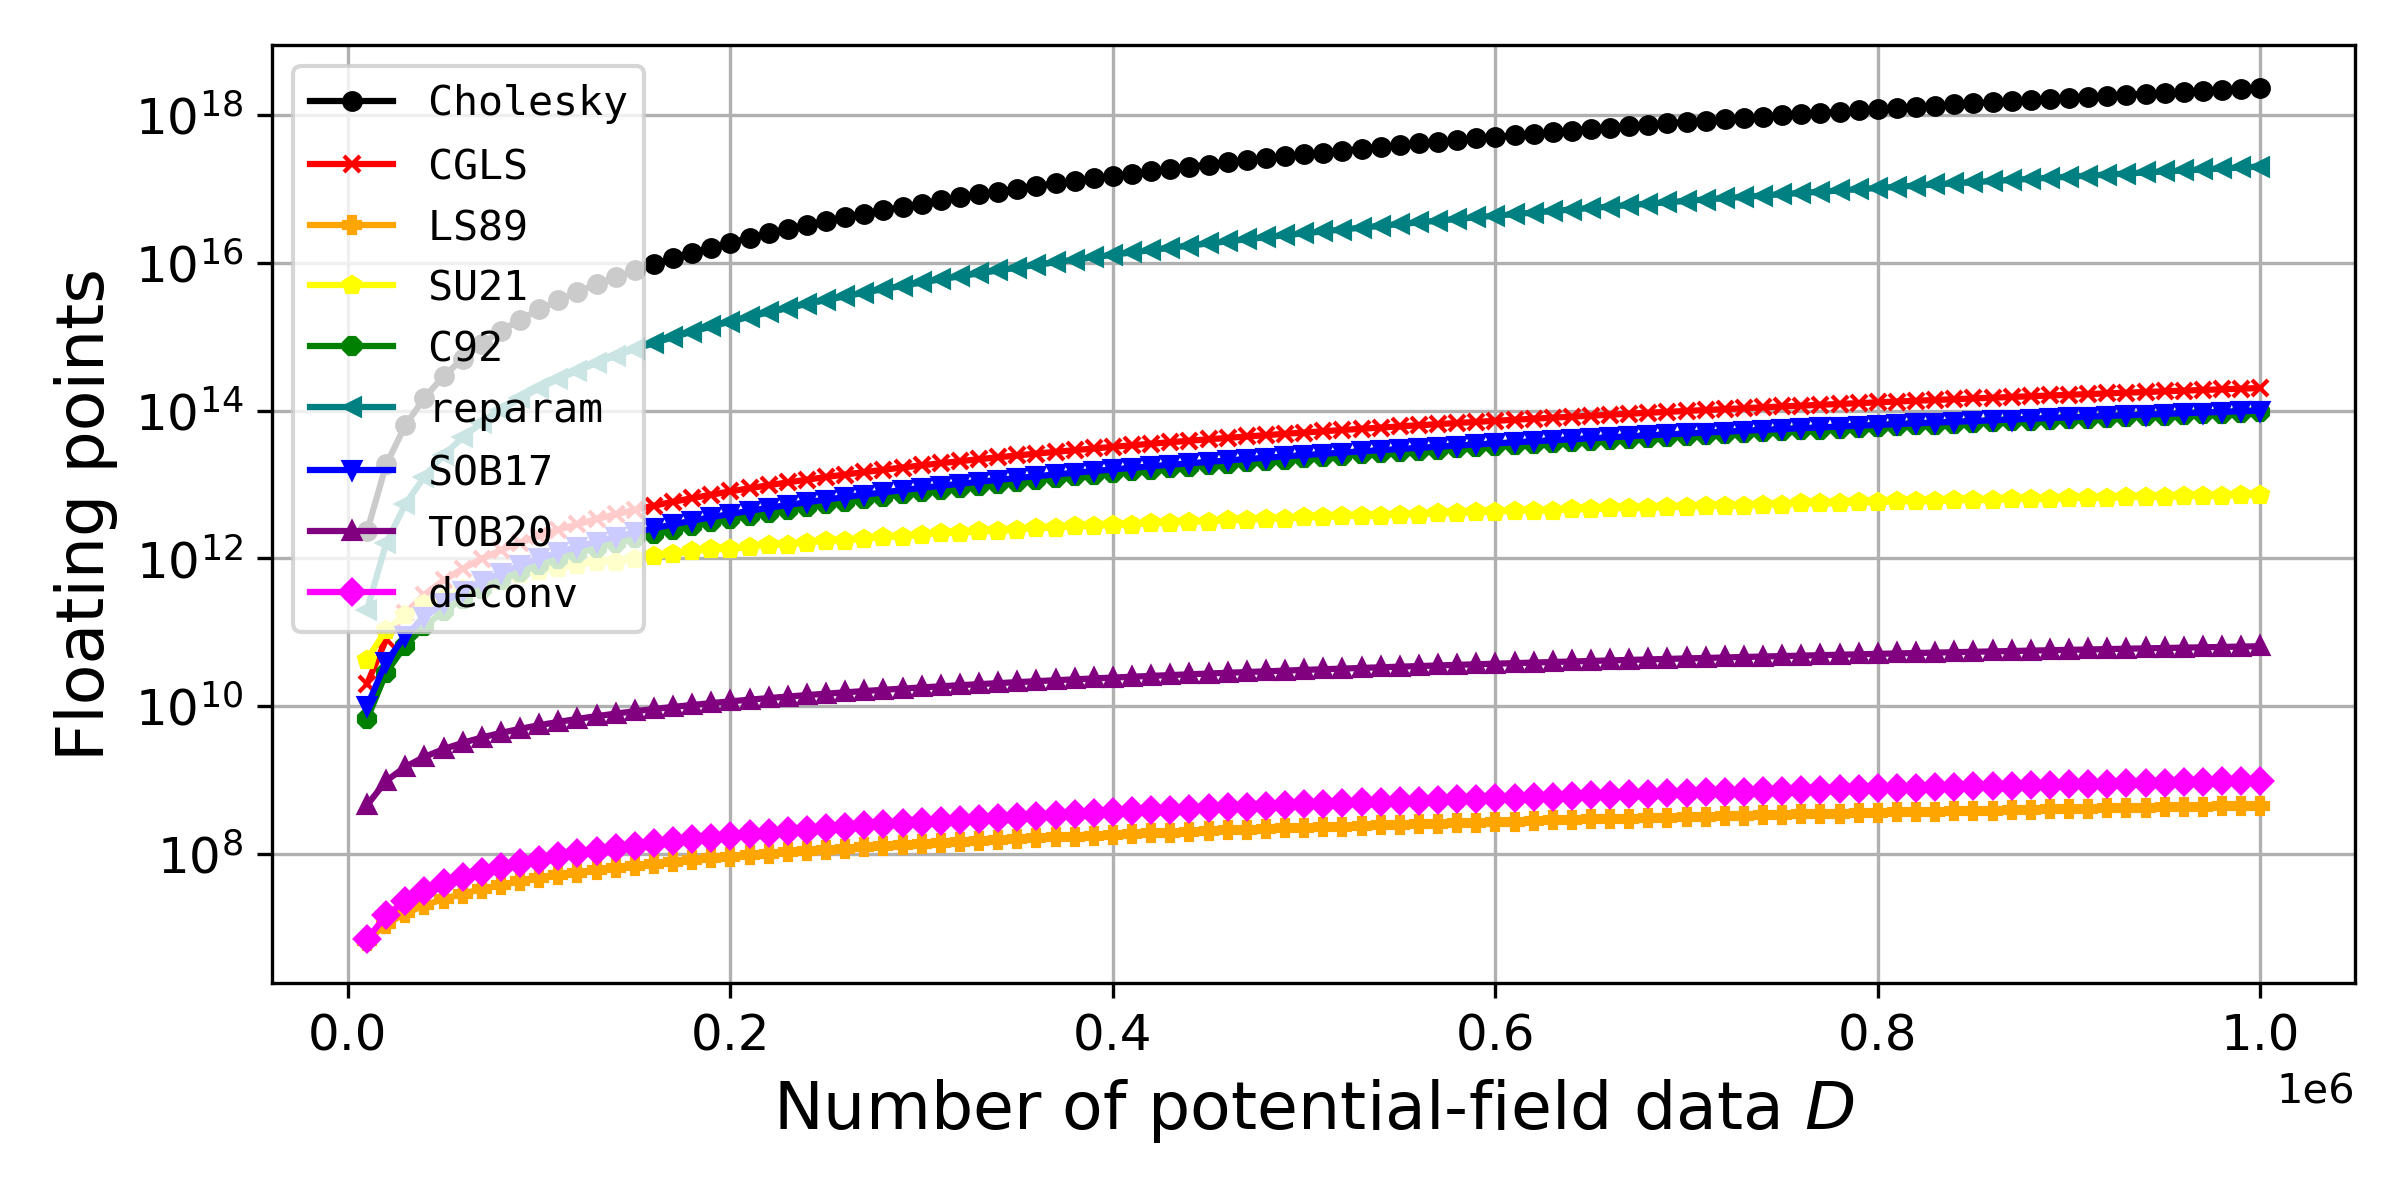
\includegraphics[width=9cm]{Fig/flops}% This is a *.eps file
\end{center}
\caption{
	Total number of flops for different equivalent-layer methods
	(equations \ref{flops:cholesky}, \ref{flops:cgls}, \ref{flops:LS89}, \ref{flops:SU21}, 
	\ref{flops:C92}, \ref{flops:reparameterization-cgls}, \ref{flops:SOB17}, \ref{flops:TOB20},
	and \ref{flops:direct-deconv}). 
	The number of potential-field data $D$ varies from $10,000$ to $1,000,000$.
	}
\label{fig:flops}
\end{figure}

%\begin{figure}[htbp]
%	\begin{center}
%		\includegraphics[width=9cm]{Fig/flops_mag}% This is a *.eps file
%	\end{center}
%	\caption{Number of \textit{flops} for many of the methods described in this work to estimate the equivalent sources using magnetic data. The range of observations varies from $10,000$ to $1,000,000$.}
%	\label{fig:2}
%\end{figure}

\begin{figure}[htbp]
	\begin{center}
			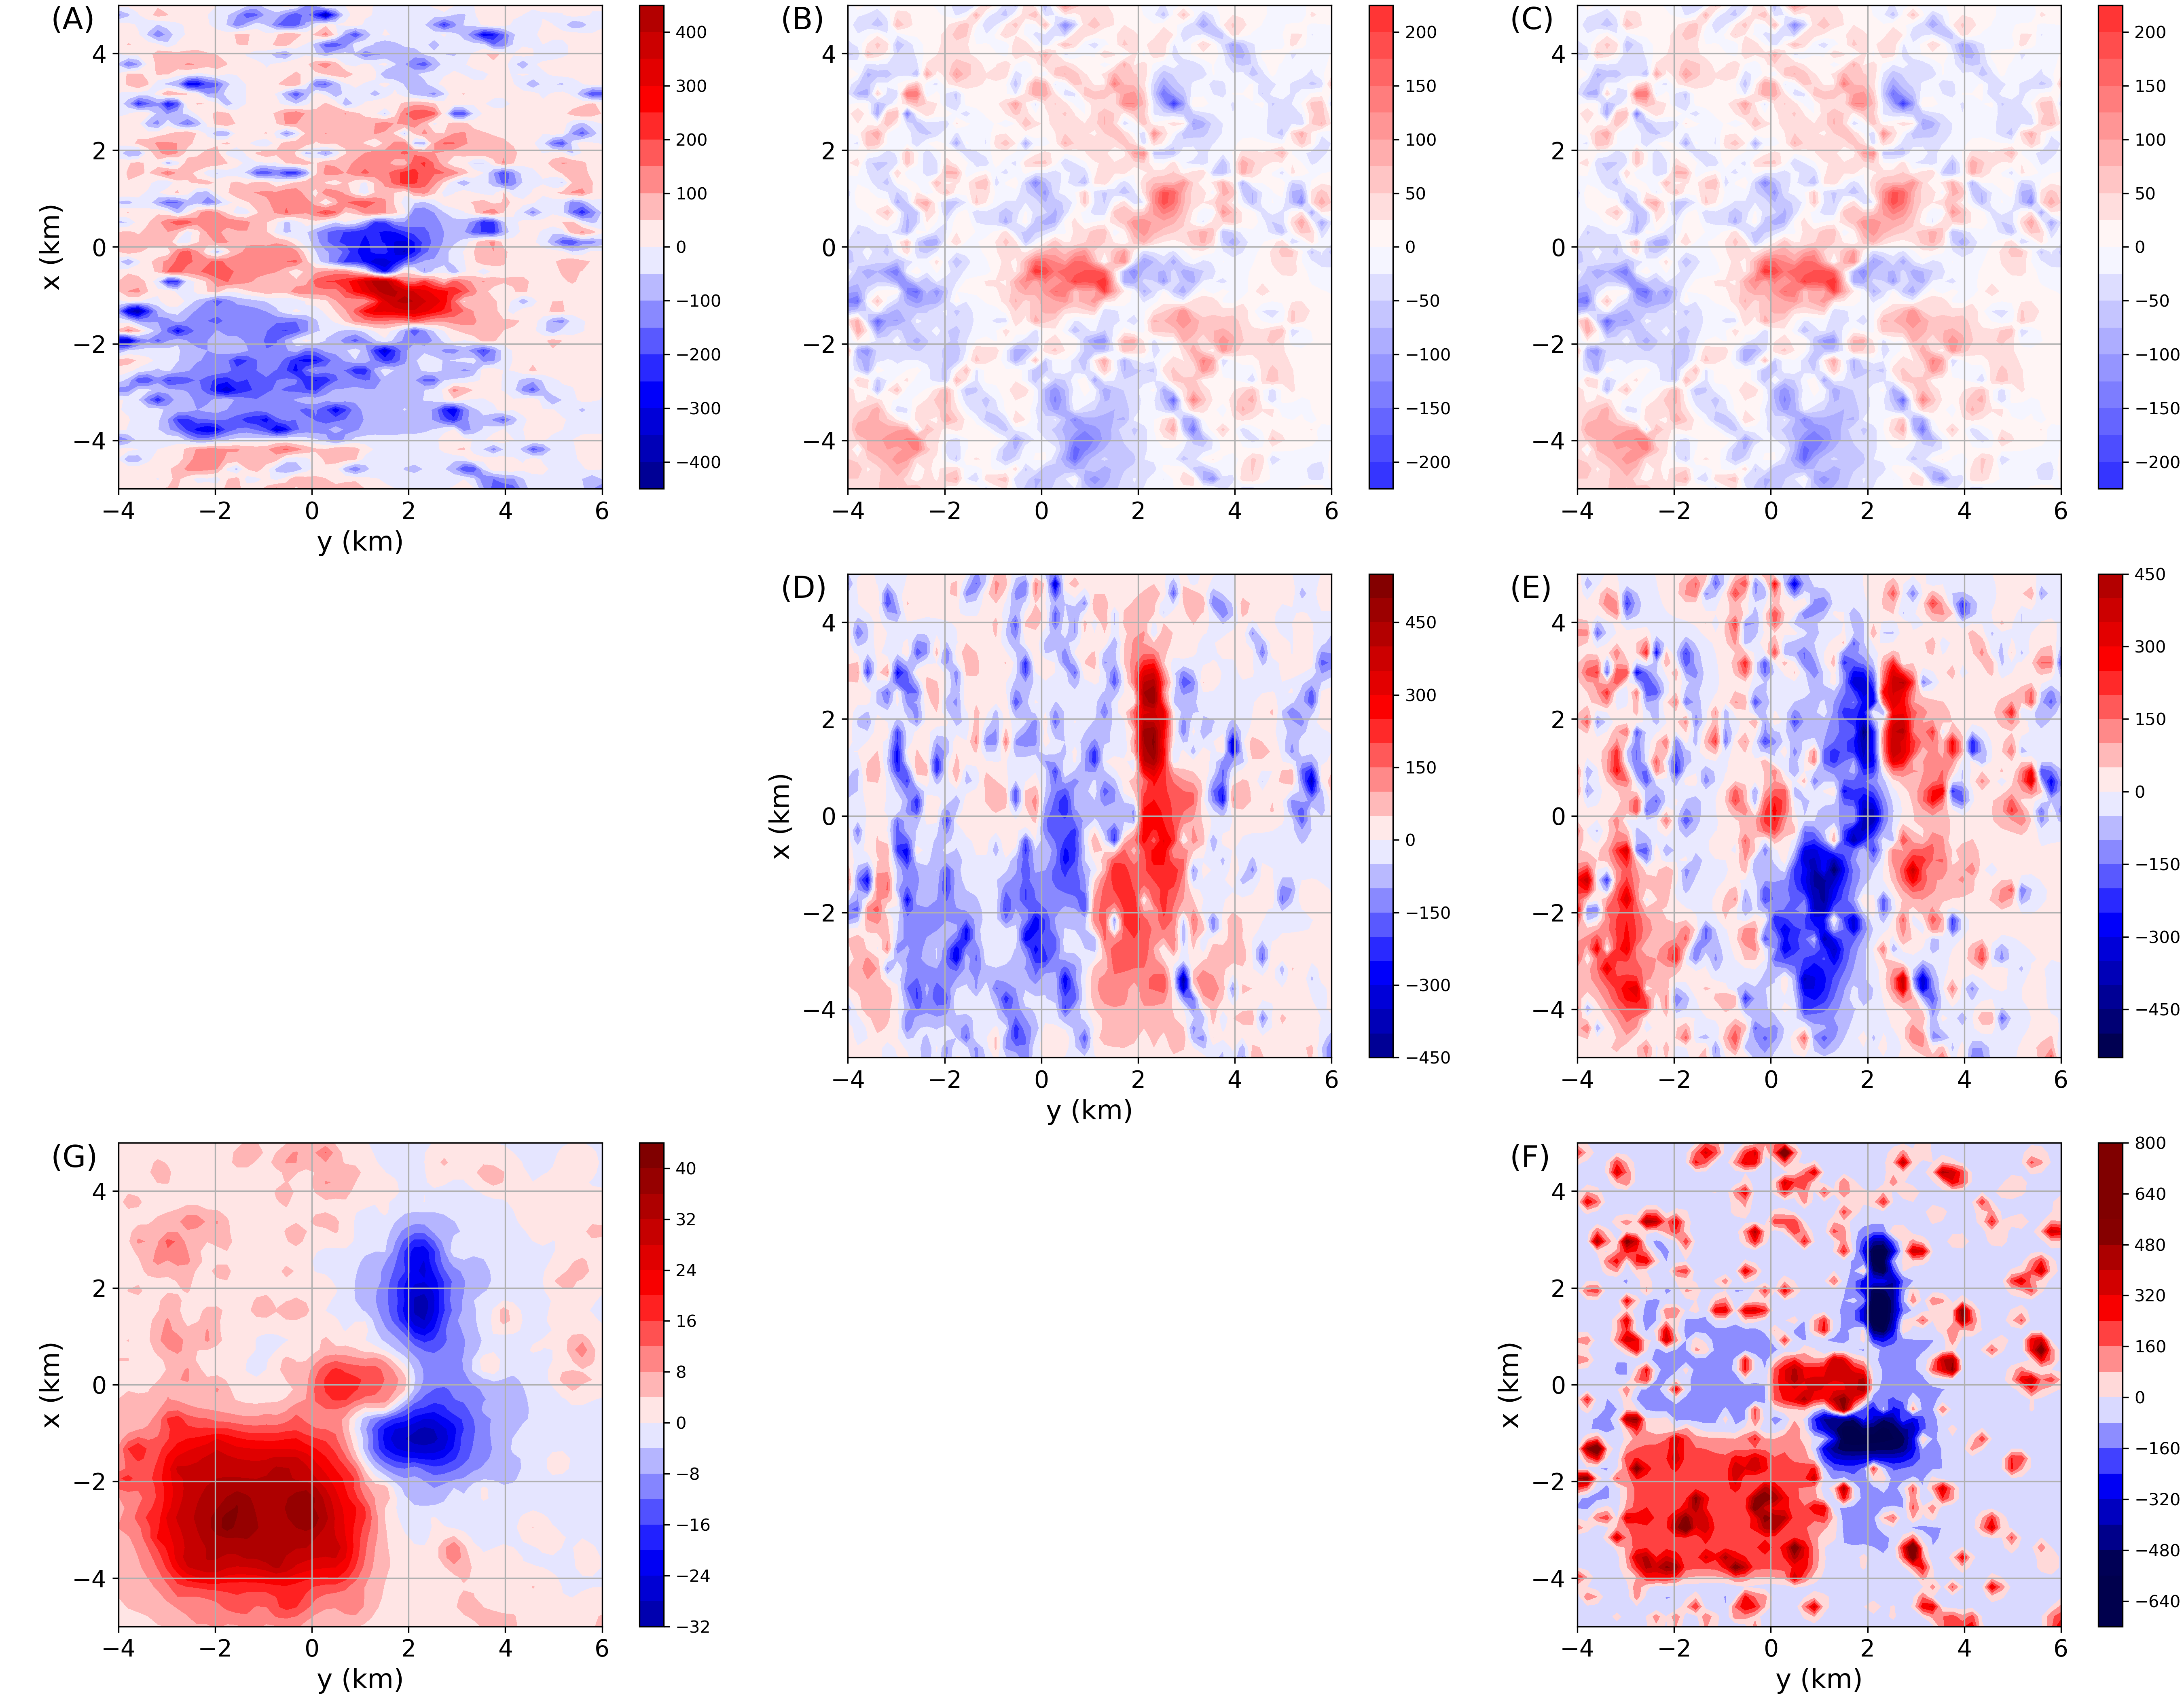
\includegraphics[width=9cm]{Fig/noise-free-data}
		\end{center}
	\caption{
		Noise-free gravity data produced by an ensemble of rectangular prisms (not shown). 
		The data are located on a regular grid of $50 \times 50$ points. 
		Panels \textbf{(A)}--\textbf{(F)} show, respectively, the $xx$, $xy$, $xz$, $yy$, $yz$ and
		$zz$ component of the gravity-gradient tensor in Eötvös (E).
		Panel \textbf{(G)} shows the gravity disturbance in milligals (mGal).
		}
	\label{fig:noise-free-data}
\end{figure}

\begin{figure}[htbp]
	\begin{center}
		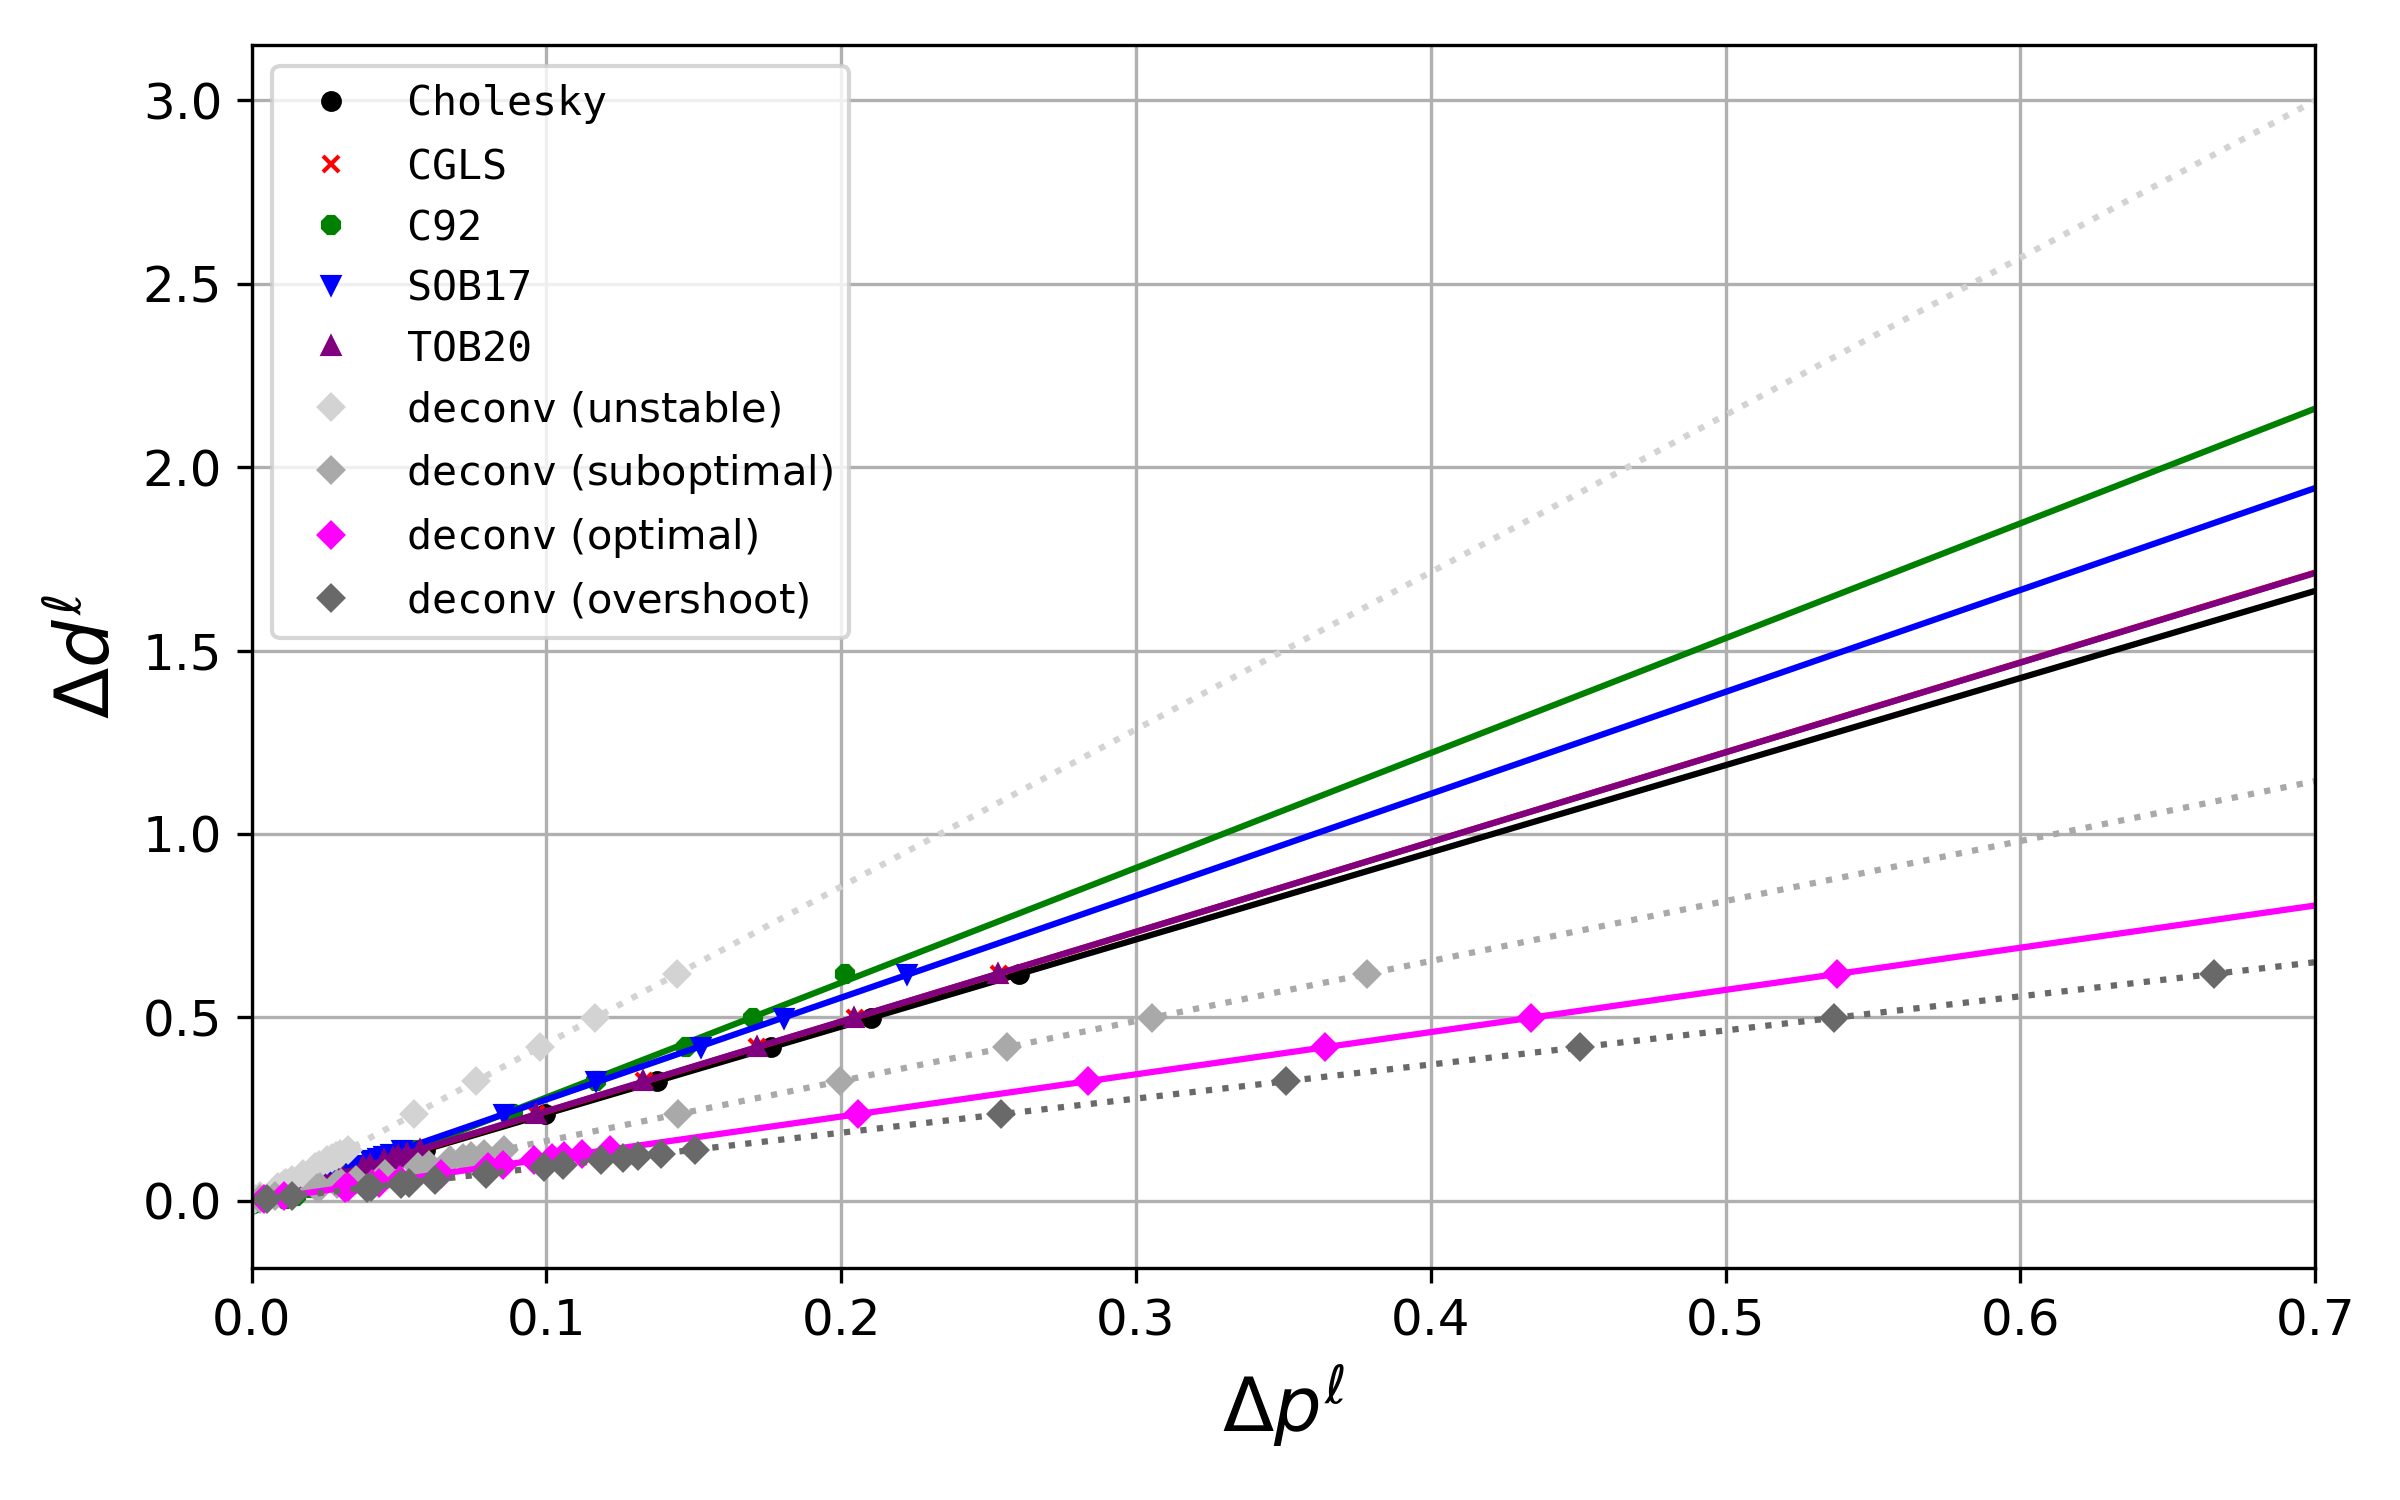
\includegraphics[width=9cm]{Fig/stability-comparison}
	\end{center}
	\caption{
		Numerical stability curves obtained for the $21$ synthetic gravity data sets 
		by using the Cholesky factorization with $\mu \approx 2 \times 10^{-2}$, 
		CGLS, iterative method (($\mathrm{SOB17}$)) and iterative deconvolution
		($\mathtt{TOB20}$) with $50$ iterations each (Algorithms \ref{alg:CGLS}, \ref{alg:SOB17} and \ref{alg:TOB20-22}) 
		and the direct deconvolution ($\mathtt{deconv.}$) computed with four different values for $\zeta$ 
		(equation \ref{eq:matrix-L-Wiener-deconvolution}): $0$, $10^{-18}$ (overshoot), $10^{-22}$ (optimal)
		and $10^{-28}$ (suboptimal).
		The stability parameter $\kappa$ (equation \ref{eq:condition-number}) obtained for the eight curves described above are $2.29$ ($\mathtt{Cholesky}$), $2.38$ 
		($\mathtt{CGLS}$), $3.25$ ($\mathtt{SOB17}$), $2.38$ ($\mathtt{TOB20}$), $4.83$, $1.59$, $1.11$ and $0.93$ ($\mathtt{deconv.}$ with null, suboptimal, optimal and overshoot 1$\zeta$).
		}
	\label{fig:stability-comparison}
\end{figure}

\begin{figure}[htbp]
	\begin{center}
		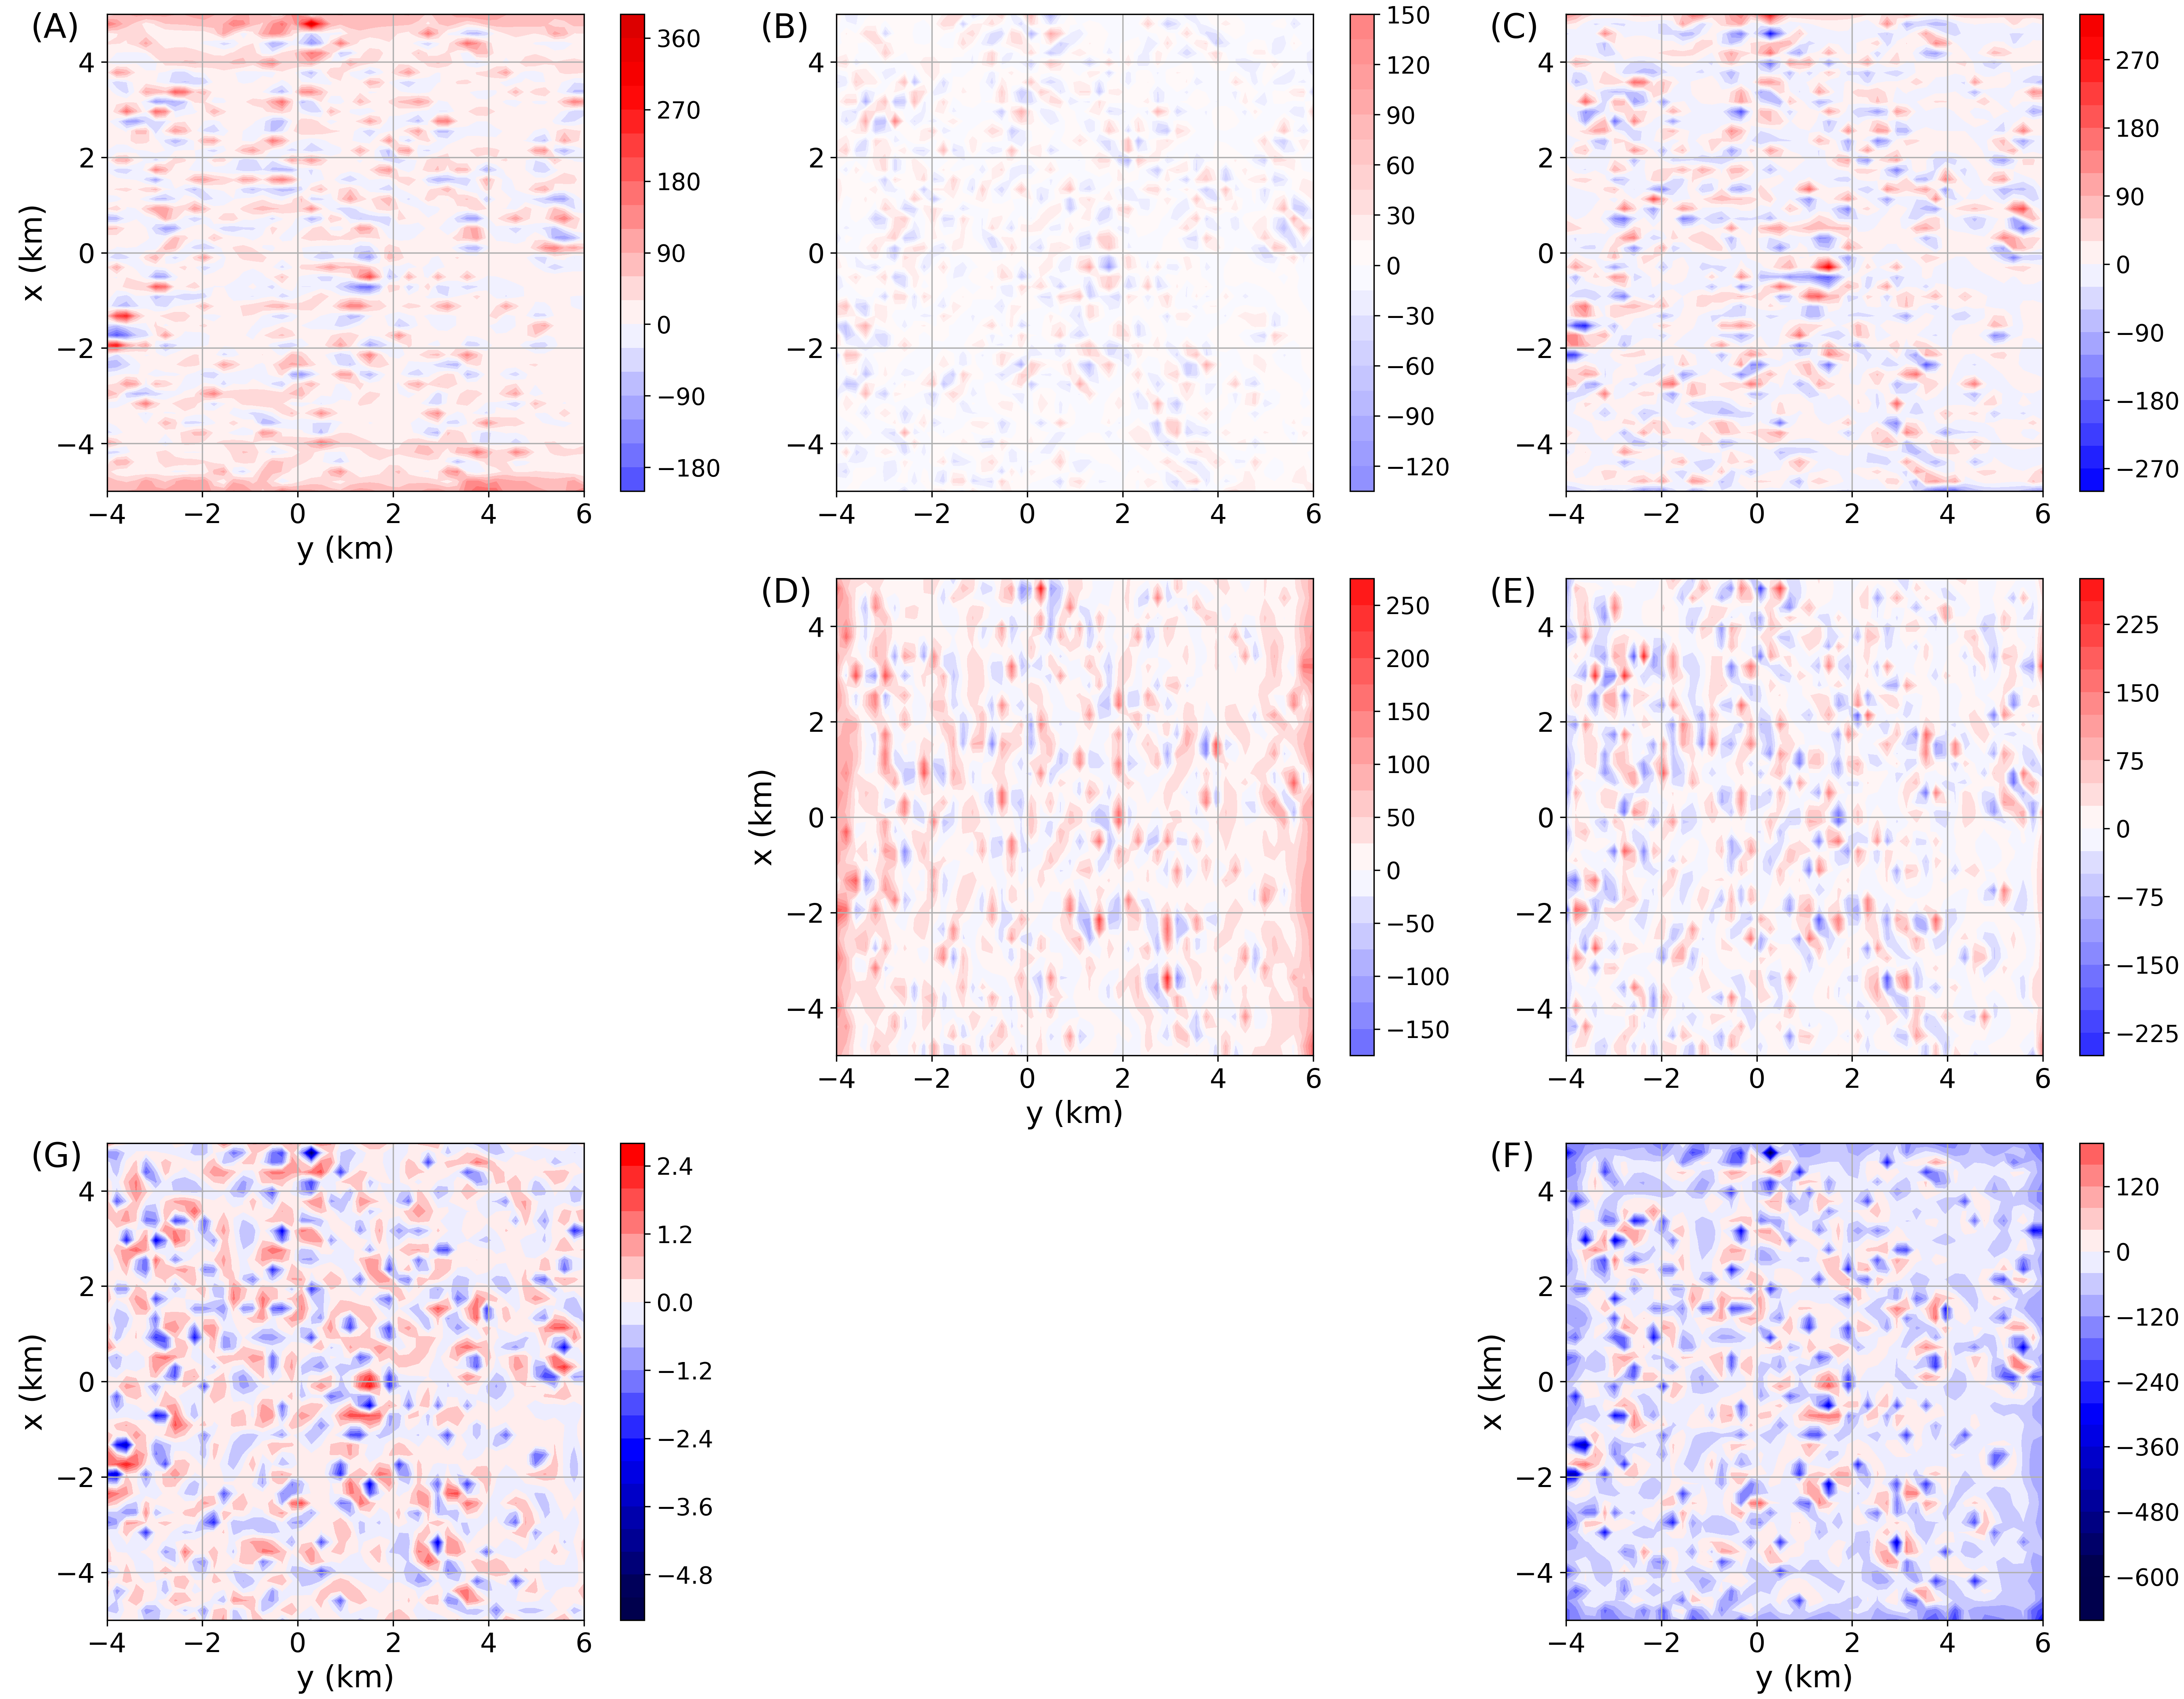
\includegraphics[width=10cm]{Fig/TOB20_residuals}
	\end{center}
	\caption{
		Residuals between the gravity data predicted by the equivalent layer estimated with the 
		iterative deconvolution ($\mathtt{TOB20}$) (Algorithm \ref{alg:TOB20-22}).
		The inverse problems was solved by using the noise-corrupted gravity 
		disturbance having the maximum noise level (not shown).
		Panels \textbf{(A)}--\textbf{(F)} show the residuals between the predicted and noise-free
		gravity gradient data (Figure \ref{fig:noise-free-data}) associated with the
		$xx$, $xy$, $xz$, $yy$, $yz$ and $zz$ components of the gravity-gradient tensor, respectively. 
		The values are in Eötvös (E).
		\textbf{(G)} Shows the residuals between the predicted and noise-corrupted gravity disturbances.
		The values are in milligals (mGal).
		}
	\label{fig:residuals-TOB20}
\end{figure}

\begin{figure}[htbp]
	\begin{center}
		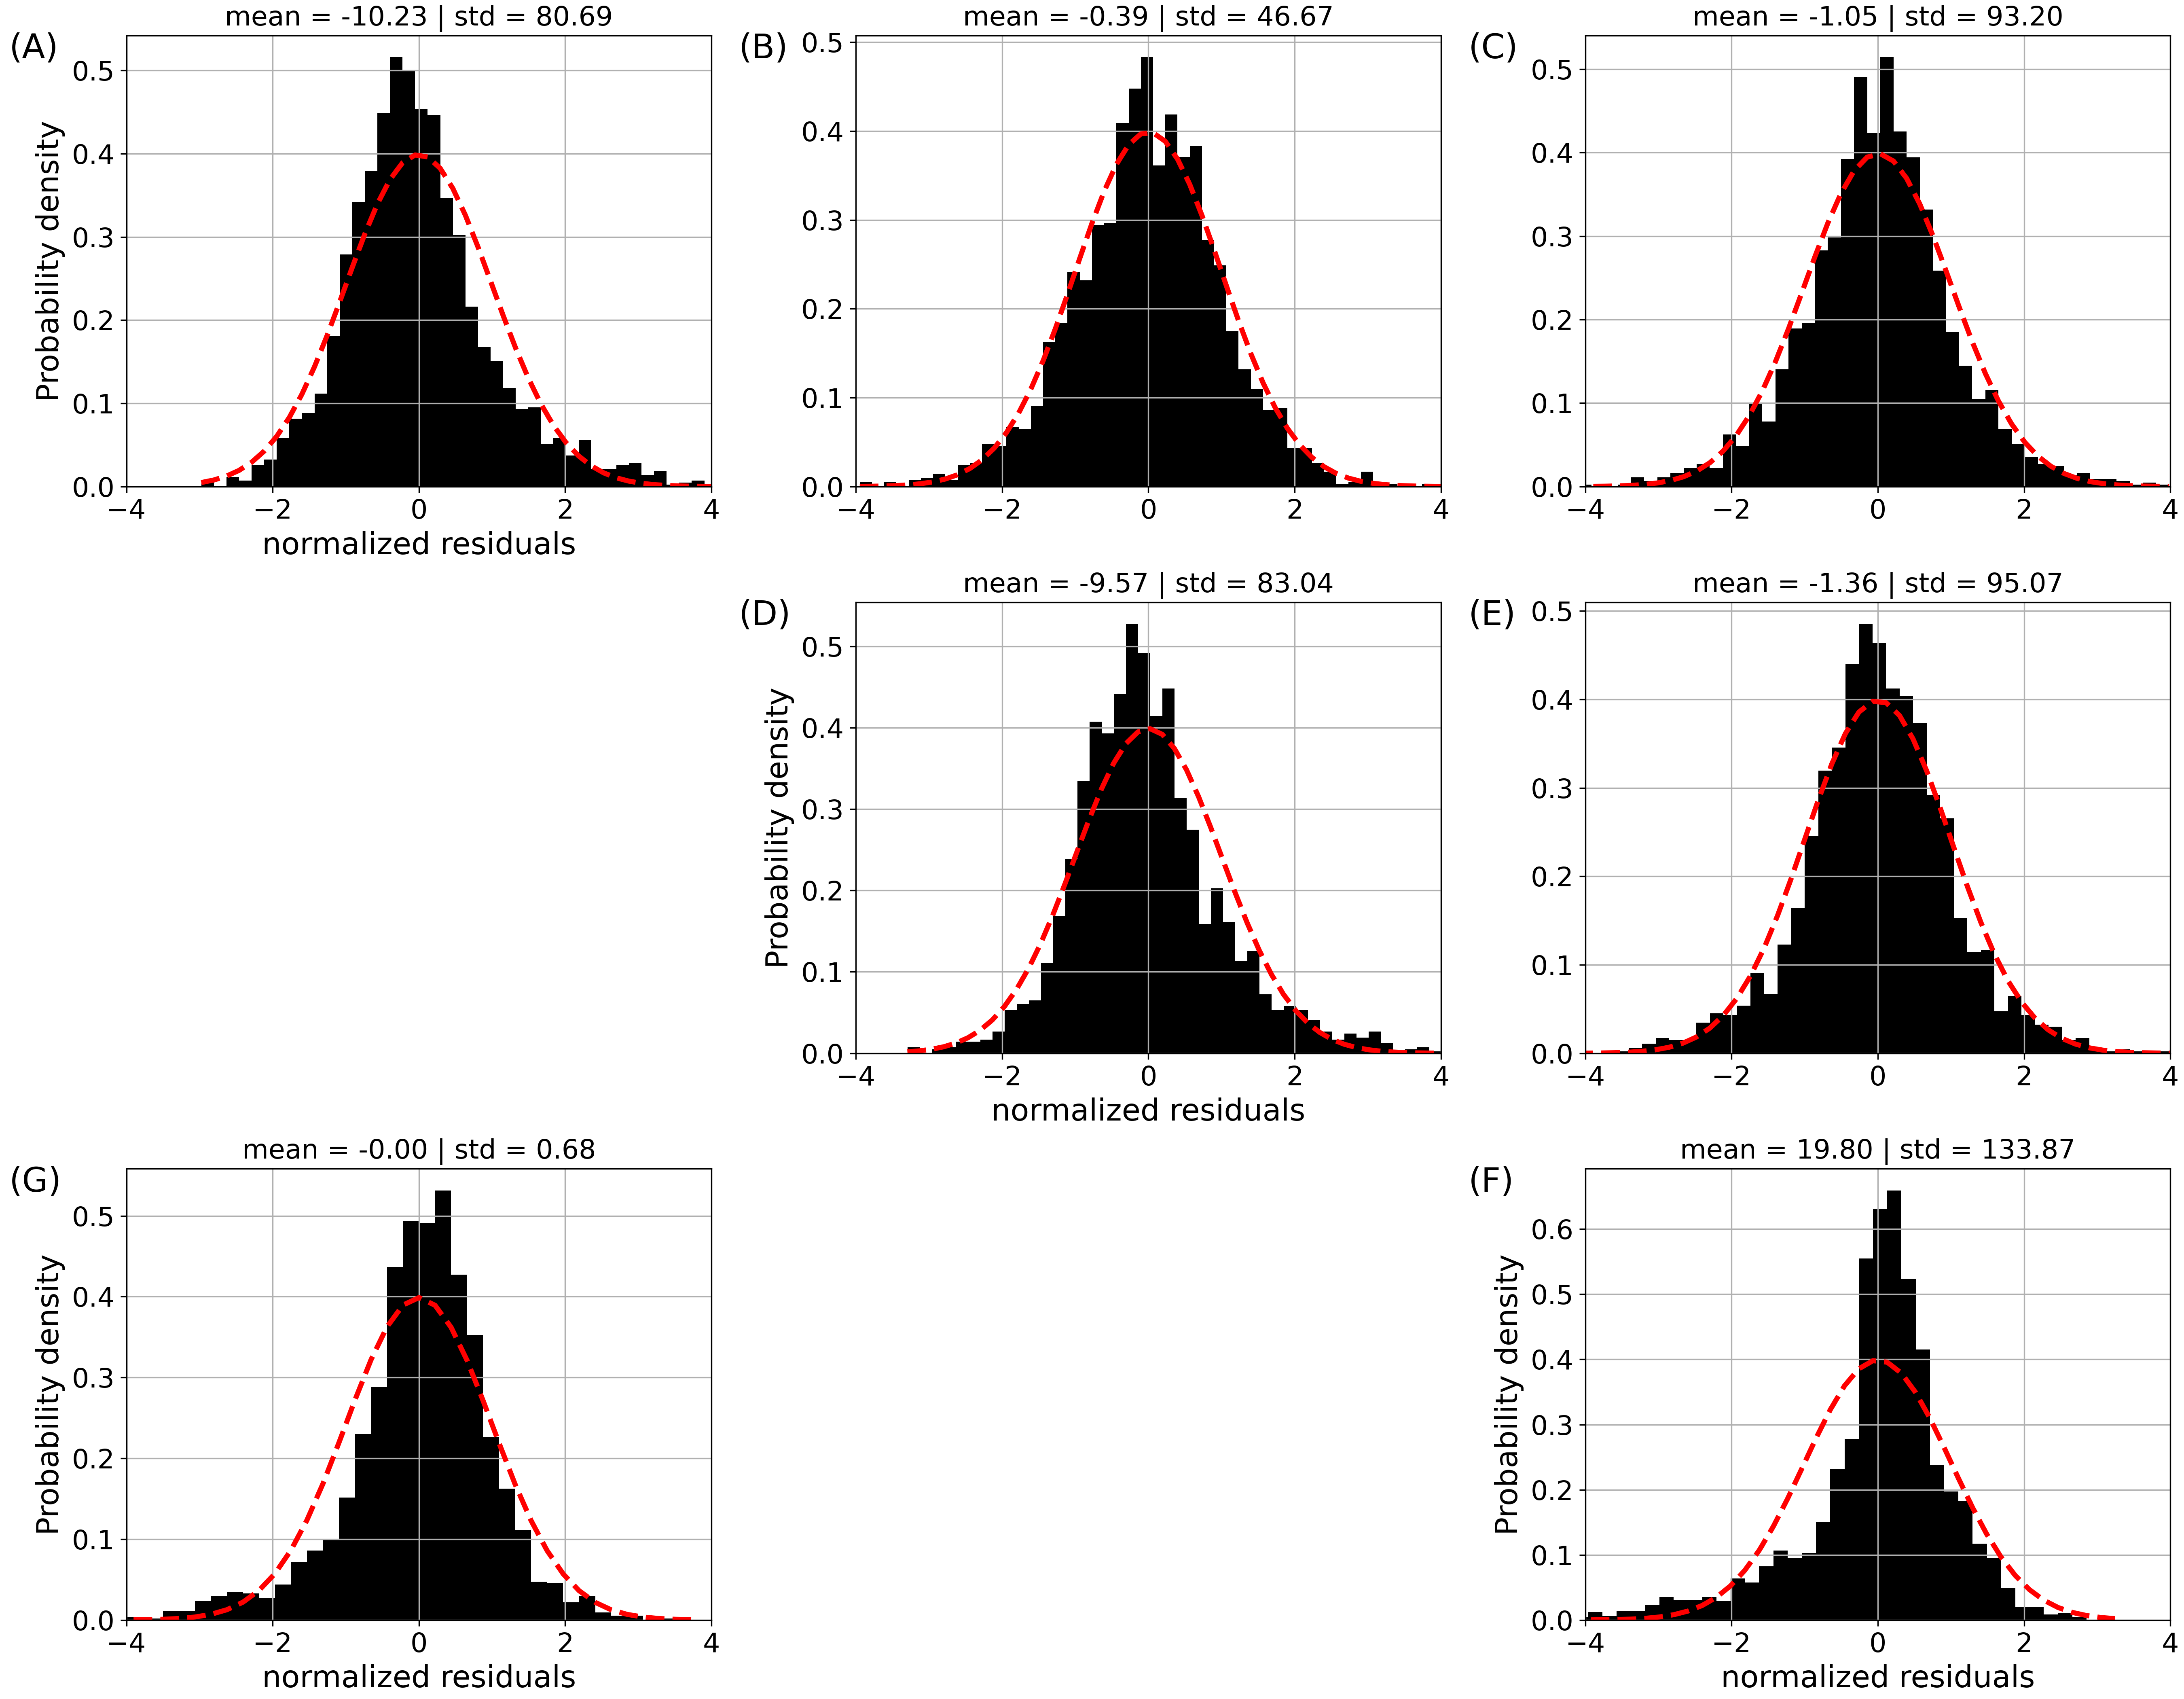
\includegraphics[width=10cm]{Fig/TOB20_histograms}
	\end{center}
	\caption{
		Histograms of the residuals shown in Figure \ref{fig:residuals-TOB20}.
		The residuals were normalized by removing the mean and dividing the difference
		by the standard deviation.
		Panels \textbf{(A)}--\textbf{(F)} show the histograms associated with the 
		$xx$, $xy$, $xz$, $yy$, $yz$ and $zz$ components of the gravity-gradient tensor, respectively. 
		\textbf{(G)} Shows the histogram of the residuals between the predicted and noise-corrupted gravity disturbances.
	}
	\label{fig:histograms-TOB20}
\end{figure}

\begin{figure}[htbp]
	\begin{center}
		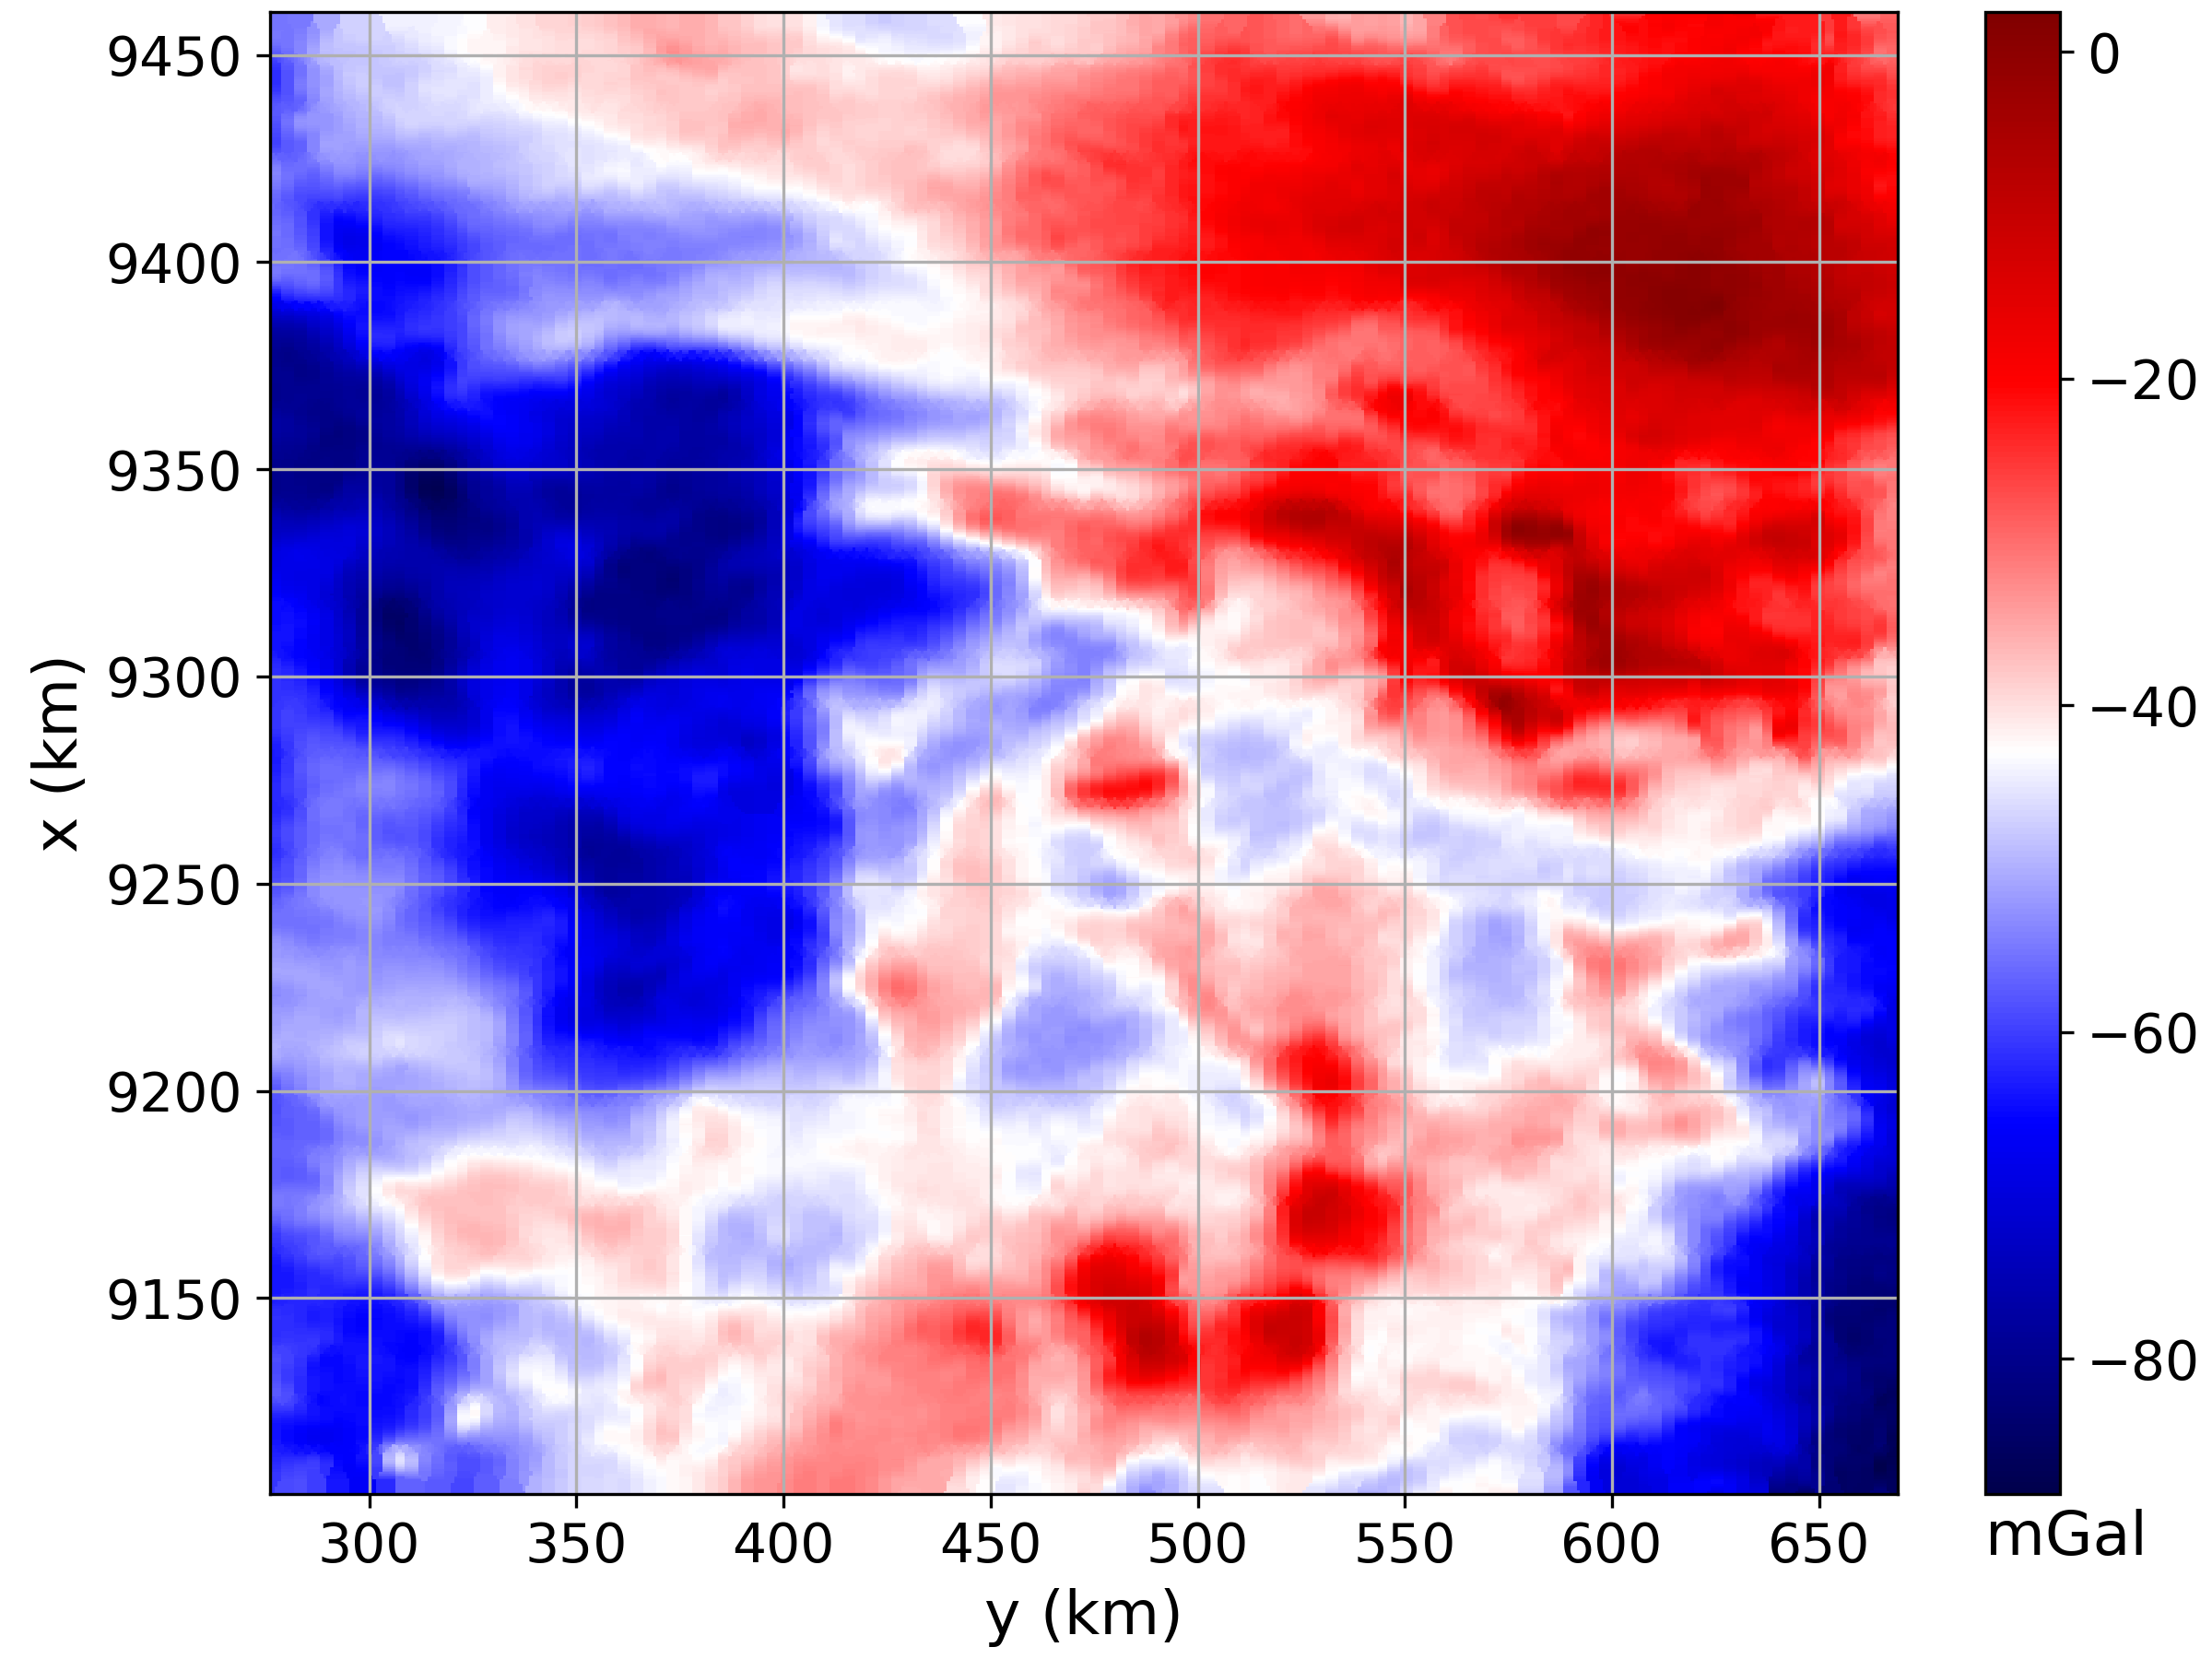
\includegraphics[width=10cm]{Fig/carajas_data}
	\end{center}
	\caption{
		Field aerogravimetric data over Caraj{\'a}s, Brazil. 
		There are $D = 500, 000$ observations located on regular grid of $1,000 \times 500$ poins.
		}
	\label{fig:carajas-data}
\end{figure}

\begin{figure}[htbp]
	\begin{center}
		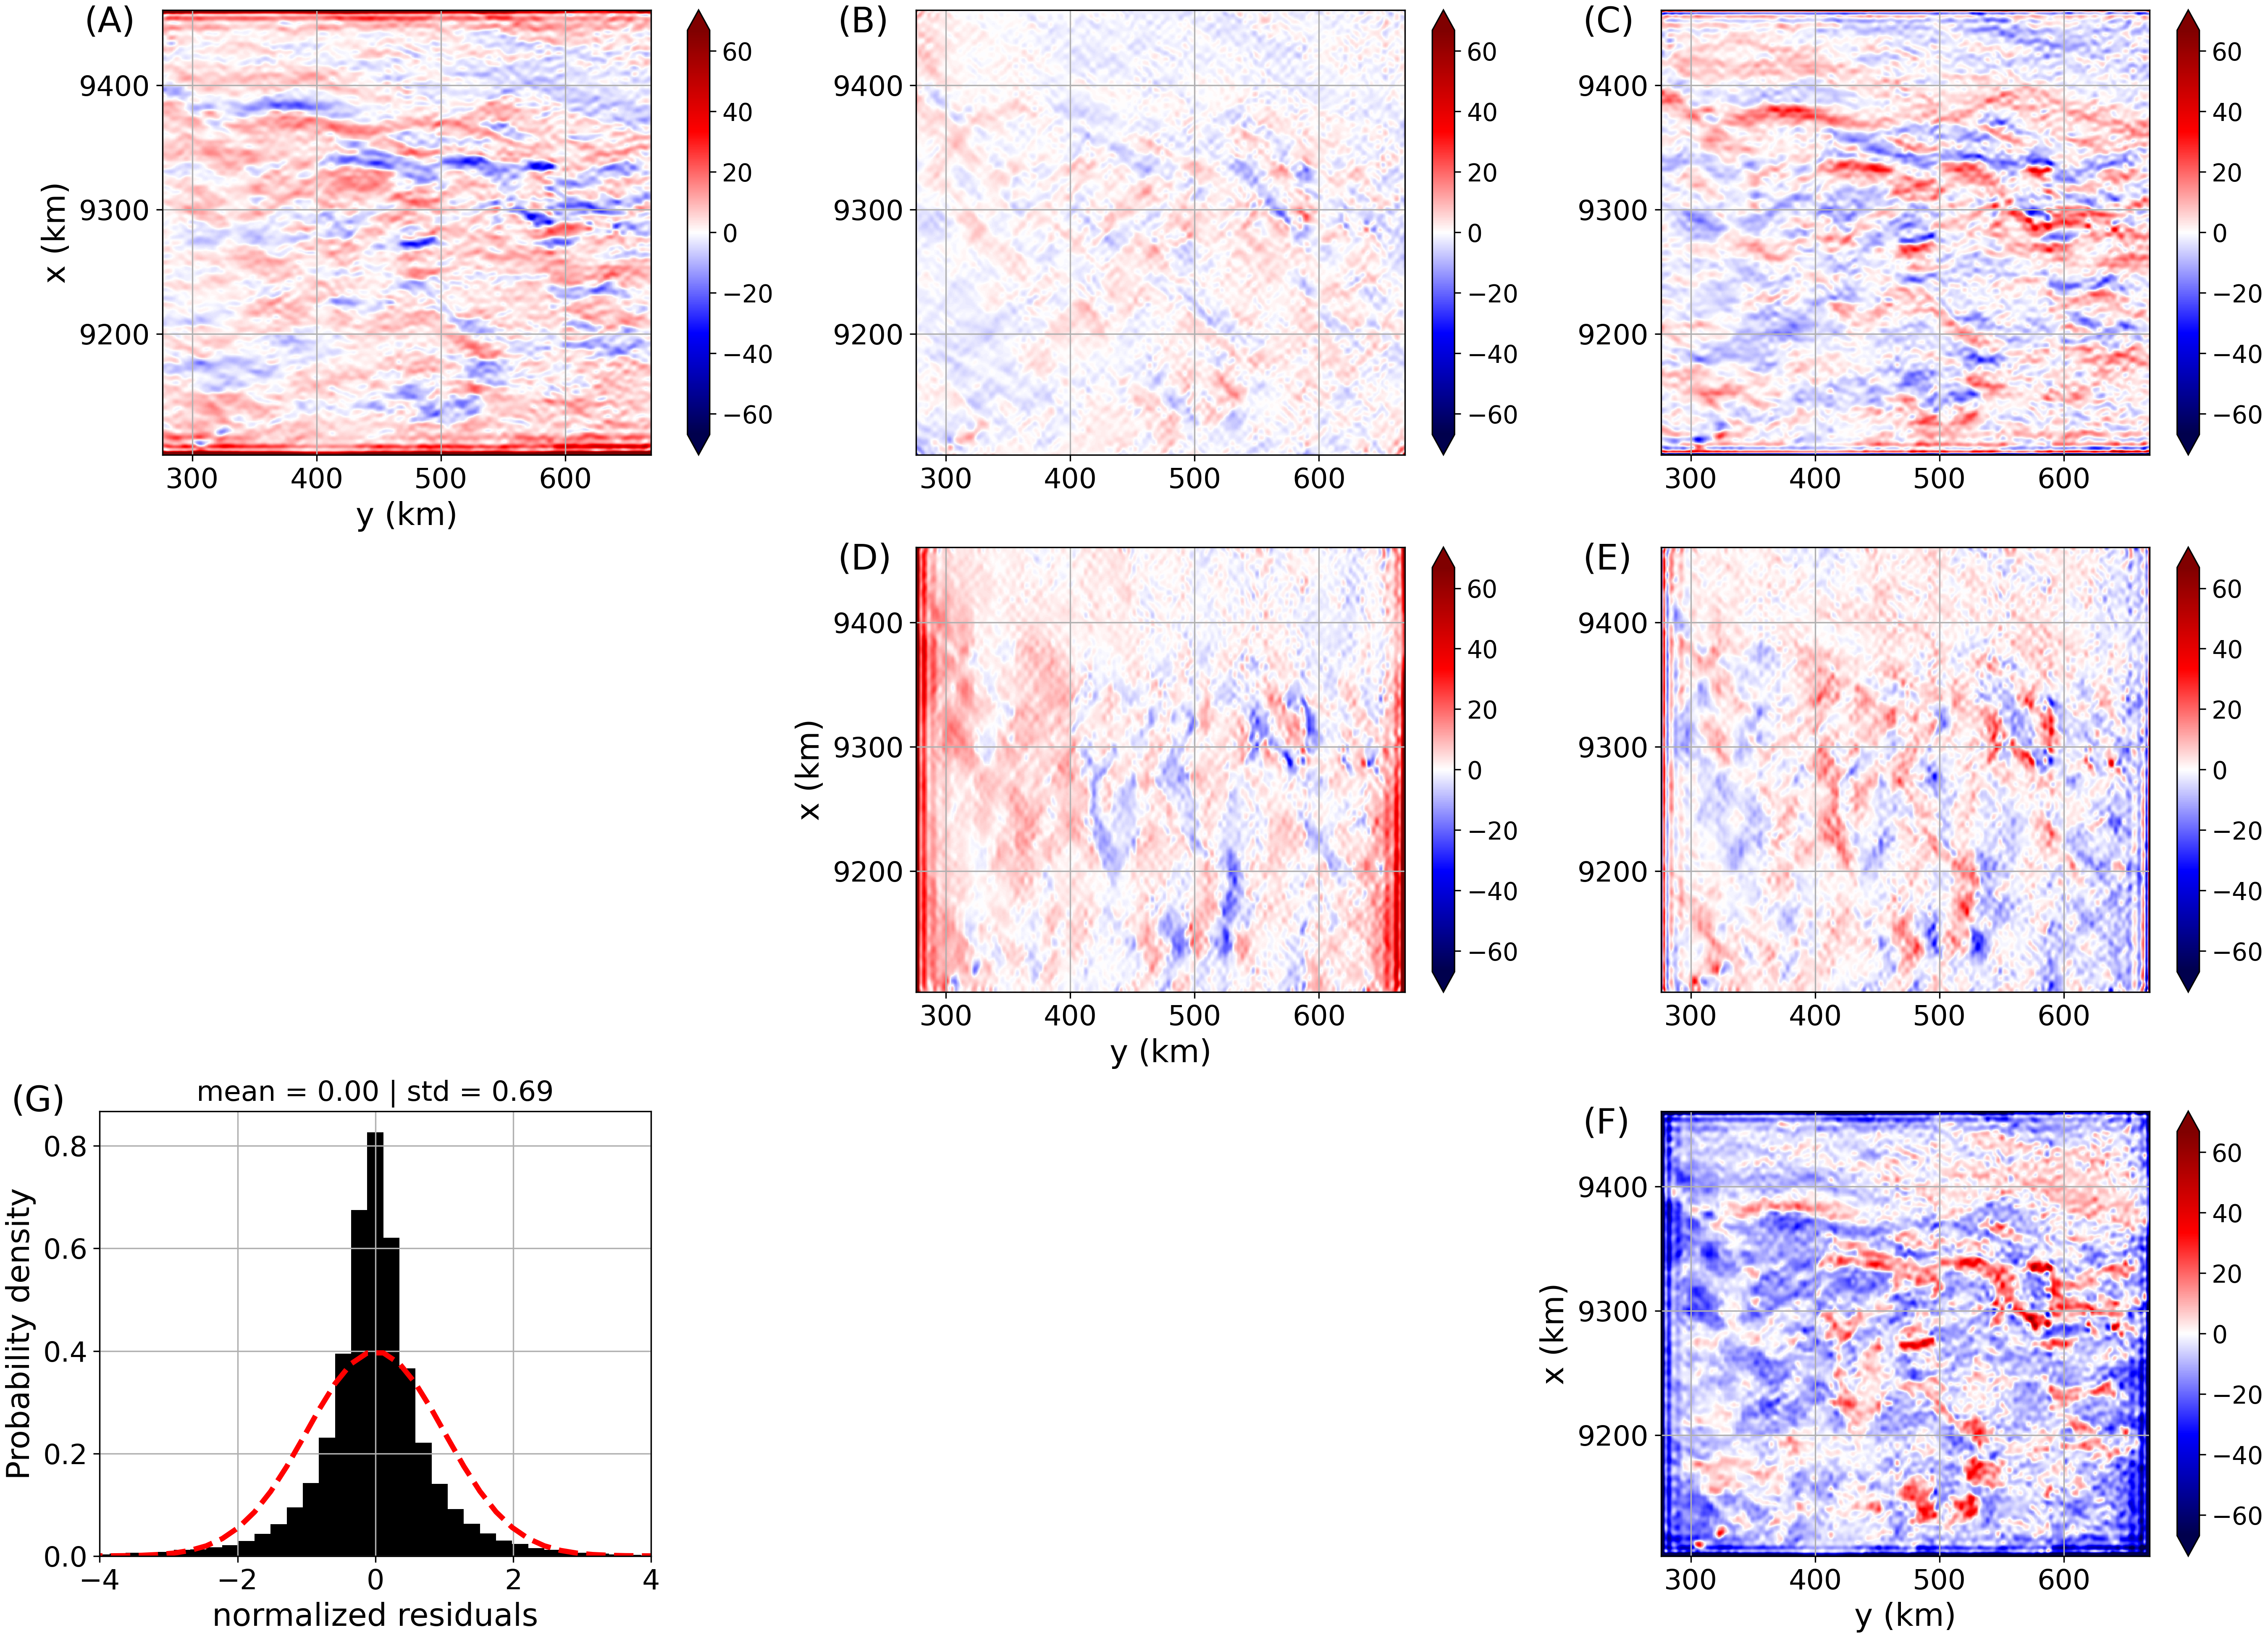
\includegraphics[width=10cm]{Fig/carajas_grav_gradient}
	\end{center}
	\caption{
		Estimated gravity-gradient tensor components over Caraj{\'a}s, Brazil.
		Panels \textbf{(A)}--\textbf{(F)} show, respectively, the $xx$, $xy$, $xz$, $yy$, $yz$ and
		$zz$ components of the gravity-gradient tensor in Eötvös (E).
		Panel \textbf{(G)} shows the histogram of the residuals between predicted data (not shown) and field data 
		(Figure \ref{fig:carajas-data}). 
		The residuals were normalized by removing the mean and dividing the difference
		by the standard deviation.
		The results were generated by applying the iterative deconvolution ($\mathtt{TOB20}$)
		(Algorithm \ref{alg:TOB20-22})
		with $50$ iterations.
		}
	\label{fig:carajas-grav-gradient}
\end{figure}

%%% If you are submitting a figure with subfigures please combine these into one image file with part labels integrated.
%%% If you don't add the figures in the LaTeX files, please upload them when submitting the article.
%%% Frontiers will add the figures at the end of the provisional pdf automatically
%%% The use of LaTeX coding to draw Diagrams/Figures/Structures should be avoided. They should be external callouts including graphics.


%\bibliographystyle{frontiersinSCNS_ENG_HUMS} %  for Science, Engineering and Humanities and Social Sciences articles, for Humanities and Social Sciences articles please include page numbers in the in-text citations
%\bibliographystyle{frontiersinHLTH&FPHY} % for Health and Physics articles
%\bibliography{test}

%\end{document}


%%% Make sure to upload the bib file along with the tex file and PDF
%%% Please see the test.bib file for some examples of references


%%% RULES FOR FIGURES


%\section*{Figure captions}
%
%%%% Please be aware that for original research articles we only permit a combined number of 15 figures and tables, one figure with multiple subfigures will count as only one figure.
%%%% Use this if adding the figures directly in the mansucript, if so, please remember to also upload the files when submitting your article
%%%% There is no need for adding the file termination, as long as you indicate where the file is saved. In the examples below the files (logo1.eps and logos.eps) are in the Frontiers LaTeX folder
%%%% If using *.tif files convert them to .jpg or .png
%%%%  NB logo1.eps is required in the path in order to correctly compile front page header %%%
%
%\begin{figure}[h!]
%\begin{center}
%
\includegraphics[width=10cm]{logo1}% This is a *.eps file
%\end{center}
%\caption{ Enter the caption for your figure here.  Repeat as  necessary for each of your figures}\label{fig:1}
%\end{figure}
%
%\setcounter{figure}{2}
%\setcounter{subfigure}{0}
%\begin{subfigure}
%\setcounter{figure}{2}
%\setcounter{subfigure}{0}
%    \centering
%    \begin{minipage}[b]{0.5\textwidth}
%        
\includegraphics[width=\linewidth]{logo1.eps}
%        \caption{This is Subfigure 1.}
%        \label{fig:Subfigure 1}
%    \end{minipage}  
%   
%\setcounter{figure}{2}
%\setcounter{subfigure}{1}
%    \begin{minipage}[b]{0.5\textwidth}
%        
\includegraphics[width=\linewidth]{logo2.eps}
%        \caption{This is Subfigure 2.}
%        \label{fig:Subfigure 2}
%    \end{minipage}
%
%\setcounter{figure}{2}
%\setcounter{subfigure}{-1}
%    \caption{Enter the caption for your subfigure here. \textbf{(A)} This is the caption for Subfigure 1. \textbf{(B)} This is the caption for Subfigure 2.}
%    \label{fig: subfigures}
%\end{subfigure}

%%% If you don't add the figures in the LaTeX files, please upload them when submitting the article.
%%% Frontiers will add the figures at the end of the provisional pdf automatically
%%% The use of LaTeX coding to draw Diagrams/Figures/Structures should be avoided. They should be external callouts including graphics.

\end{document}
